%\documentclass[AMA,Times1COL]{WileyNJDv5} %STIX1COL,STIX2COL,STIXSMALL
\documentclass[CHICAGO,Times1COL]{WileyNJDv5} %STIX1COL,STIX2COL,STIXSMALL
%\documentclass[APA,Times1COL]{WileyNJDv5} %STIX1COL,STIX2COL,STIXSMALL


\usepackage{kotex} % To ensure proper Korean typesetting

\articletype{Empirical Research Article}%

\RequirePackage{etoolbox}

% #################### Conditional formatting ############################

% Most conditional text formatting is implemented using Boolean Expressions provided by the etoolbox package 
% See ftp://ftp.funet.fi/pub/TeX/CTAN/macros/latex/contrib/etoolbox/etoolbox.pdf for examples 
% See small example 1 at http://tex.stackexchange.com/questions/5894/latex-conditional-expression 
% See small example 2 at http://notesofaprogrammer.blogspot.fi/2014/10/conditional-processing-of-latex.html  


% Shall the boxes arround submited content be displayed? 
% Such boxes are invoked in the document with the 'submitedtext' enviroment and the 'SubmittedNote' command 


\newtoggle{boxSubmittedContent}


%\toggletrue{boxSubmittedContent}
\togglefalse{boxSubmittedContent} 
 



% Is this the draft or the final version 

\newtoggle{draftVersion}



% Uncomment for draft mode 
%\toggletrue{draftVersion}

% Uncomment for final version 
\togglefalse{draftVersion}


\newtoggle{IS-Audience}


% Uncomment IS Audience 
\toggletrue{IS-Audience}
%\togglefalse{IS-Audience}




\newtoggle{SeCo-Audience}



% Uncomment for draft mode 
%\toggletrue{SeCo-Audience}
\togglefalse{SeCo-Audience}


\newtoggle{shortVersion}
\toggletrue{shortVersion}
%\togglefalse{shortVersion}

% Uncomment for final version 




%%%%%%%%%%%%%%%%%%%%%%%%%%%%%%%%%%%%%%%%%%%%%%%%%%%%%%%%%%%%%%%%%%%%%%%%%%%%%%%%%%%%%%%%%%%%%%%%
%%%%%%   Should Figures and tables  be places on site? Or in the end of the document?  %%%%%%%%%
%%%%%%%%%%%%%%%%%%%%%%%%%%%%%%%%%%%%%%%%%%%%%%%%%%%%%%%%%%%%%%%%%%%%%%%%%%%%%%%%%%%%%%%%%%%%%%%%

% bolean conditional that sets tables and figures on site vs vs on document  
\newtoggle{TaFigOnEnd}


\toggletrue{TaFigOnEnd}
%\togglefalse{TaFigOnEnd}

% Uncommend if figures and tables should be on end 
%\TaFigOnEndtrue

% Uncommend if figures and tables should be on end 
%\TaFigOnEndfalse 




%\usepackage[hidelinks]{hyperref}


\usepackage{tabularx}
\usepackage{booktabs}
\usepackage[flushleft]{threeparttable}

\usepackage{acronym}

% Capitalization of titles
%\usepackage{stringstrings}
%\usepackage{mfirstuc}
\usepackage{mfirstuc-english}



%%%%%%%%%%%%%%%%%%%%%%%%%%%%%%%%%%%%%%%%%%%%%%%%%%%%%%%%%%%%%%%%%%%%%%%%%%%%%%%%%%%%%%%
%%%%%%%  For noting of which, where and when content was submitted / published %%%%%%%%
%%%%%%%%%%%%%%%%%%%%%%%%%%%%%%%%%%%%%%%%%%%%%%%%%%%%%%%%%%%%%%%%%%%%%%%%%%%%%%%%%%%%%%%

% Author Jose Teixeira <japolinario@gmail.com> 20 Oct 2016 

%\usepackage[dvipsnames]{xcolor}
\usepackage[many]{tcolorbox}
\usepackage{marginnote}
\usepackage{framed}
\usepackage{float}





% Make nice boxes 
%# 2 is color 
%# 3 is title  
\newtcolorbox[]{subAndRevbox}[3][]
{
  colframe = #2,
  colback  = #2!10,
  coltitle = #2!20!black,  
  fonttitle=\bfseries\color{Brown},
  title    = \footnotesize  #3,
  #1,
}




%%%%%%%%% FIGURES  %%%%%%%%%%%%%%%%%%%



% Add a boxed note to  highlight that the Figure was submitted somewhere.
% Argument Journal and/or Date submitted 
\newenvironment{submittedFigure}[1][Submitted somewhere]
    {  % Before the figure 
      \iftoggle{boxSubmittedContent}{%
      \centering 
      % boxes showing were it was submited     
      \begin{minipage}{1.0\textwidth}
      %\begin{framed}\raggedleft%\centering -> error not in par mode errot       
      \begin{subAndRevbox}{Melon}{ \centering Figure as submitted to #1}
      }
      {% Otherwise there is nothing to highlight 
      }

  }
  {  % After the figure 
  
       \iftoggle{boxSubmittedContent}{%
       % boxes arround the submitted figure are to be displayed
     
      \end{subAndRevbox} %error 
      % \end{framed} error 
      \end{minipage}
       
      }
      {% Otherwise there is nothing to highlight 
      }
}

%%%%%%%%% Tables %%%%%%%%%%%%%%%%%%%



% Add a boxed note to  highlight that a table was submitted somewhere.
% Argument can be the Journal and/or Date submitted  where the table was submited
\newenvironment{submittedTable}[1][Submitted somewhere]
    {  % Before the figure 
      \iftoggle{boxSubmittedContent}{%
      \centering 
      % boxes showing were it was submited     
      \begin{minipage}{1.0\textwidth}
      %\begin{framed}\raggedleft%\centering -> error not in par mode errot       
      \begin{subAndRevbox}{Melon}{ \centering Table as submitted to #1}
      }
      {% Otherwise there is nothing to highlight 
      }

  }
  {  % After the figure 
  
       \iftoggle{boxSubmittedContent}{%
       % boxes arround the submitted figure are to be displayed
     
      \end{subAndRevbox} %error 
      % \end{framed} error 
      \end{minipage}
       
      }
      {% Otherwise there is nothing to highlight 
      }
}

%%%%%%%%%%%%%%%%%%%%%%%%%%%%%%%%%%%%%%%%%%%%%%%%%%%%%%%%%%%%%%%%%%%%%%%%%%%%%%%%%%%%%%%%%%%%%%%%%%%%%%%%%%%
%%%%%%%%%% Enables support of track changes, marking of draft text and review comments %%%%%%%%%%%%%%%%%%%%
%%%%%%%%%%%%%%%%%%%%%%%%%%%%%%%%%%%%%%%%%%%%%%%%%%%%%%%%%%%%%%%%%%%%%%%%%%%%%%%%%%%%%%%%%%%%%%%%%%%%%%%%%%%

% Author Jose Teixeira <japolinario@gmail.com> 20 Oct 2016


\usepackage{xargs} 
%\usepackage[dvipsnames]{xcolor}

\usepackage{stackengine}

% 
%\RequirePackage[]{todonotes}
\RequirePackage[obeyDraft]{todonotes} % with obay draft todonotes apear only in draft mode
%\usepackage[]{todonotes}


%%%%%%%%%%%%%%%% Based on the todonotes packacke  %%%%%%%%%%%%%%%%%%%%%%%%%%%%

%The pack­age pro­vides ex­tended ver­sions of \new­com­mand and re­lated LaTeX com­mands, which al­low easy and ro­bust def­i­ni­tion of macros with many %op­tional ar­gu­ments, us­ing a clear and sim­ple xkey­val-style syn­tax.


% %The pack­age lets the user mark things to do later, in a sim­ple and vi­su­ally ap­peal­ing way
% \usepackage[colorinlistoftodos,prependcaption,textsize=tiny]{todonotes}
% 
% % Uncomment to disable the todo lists and marks - 
% %\usepackage[disable, colorinlistoftodos,prependcaption,textsize=tiny]{todonotes}

%% It a good practice to couple this with a config.tex file 

\newcommandx{\error}[2][1=]{\todo[linecolor=red,backgroundcolor=red!50,bordercolor=red,#1]{#2}}
\newcommandx{\unsure}[2][1=]{\todo[linecolor=red,backgroundcolor=red!25,bordercolor=red,#1]{#2}}
\newcommandx{\change}[2][1=]{\todo[linecolor=blue,backgroundcolor=blue!25,bordercolor=blue,#1]{#2}}
\newcommandx{\info}[2][1=]{\todo[linecolor=green,backgroundcolor=green!25,bordercolor=green,#1]{#2}}
\newcommandx{\improvement}[2][1=]{\todo[linecolor=green,backgroundcolor=green!25,bordercolor=green,#1]{#2}}
\newcommandx{\thiswillnotshow}[2][1=]{\todo[disable,#1]{#2}}

% This places the todonotes in the left
%\reversemarginpar

% Usage example I: \error{it's seems with two ee, not one e}{seems no sems}
% Usage example II: \improvement{To jose: Consider to find a good reference}{Swans are never black} 


%%%%%%%%%%%%%%%%%%%%%%%%%%%%%%%%%%%%%%%%%%%%%%%%%%%%%%%%%%%%%%%%%%%%%%%%%%%%%%

%%%%%%%%%%%%%%%% Simply  marking draft text in the violet color %%%%%%%%%%%%%%%%%%%%%%%%%%%%

% Environment to draft text 
\newenvironment{drafte} {\color{violet}}

% Usage example:  \begin{drafte} block of text in draft mode \end{drafte}                                 

%%%%%%%%%%%%%%%%%%%%%%%%%%%%%%%%%%%%%%%%%%%%%%%%%%%%%%%%%%%%%%%%%%%%%%%%%%%%%%%%%%%%%%%%%%%%
   
% Command to mark a paragraph as draft   
\newcommand{\draftp}[1]{\textcolor{violet}{#1}}  

% Usage example: \draftp{ This paragraph of text is still a drtaft }


%%%%%%%%% Based on discussion as https://tex.stackexchange.com/questions/142242/robust-way-to-mark-draft-text/142258 %%%%%%%%%%%

% Allows to make marks above and bellow the text -- to support review or warning authors. 

\setstackgap{L}{.5\baselineskip}
\newcommand\markabove[2]{{\sffamily\color{red}\hsmash{$\uparrow$}%
  \smash{\toplap{#1}{\scriptsize\bfseries#2}}}}
\newcommand\markbelow[2]{{\sffamily\color{red}\hsmash{$\downarrow$}%
  \smash{\bottomlap{#1}{\scriptsize\bfseries#2}}}}
  
% Usage examples I: \markbelow{l}{and lapped, I think} <--mark comments below to the left 
% Usage examples II: \markbelow{c}{and lapped, I think} <--mark  comments below centered over 
% Usage examples II: \markabove{r}{I'm sorry, but the links didn't show}%  <--mark  comments above to the right 
%%%%%%%%%%%%%%%%%%%%%%%%%%%%%%%%%%%%%%%%%%%%%%%%%%%%%%%%%%%%%%%%%%%%%%%%%%%%%%%%%%%%%%%%%%%%%%%%%%%%%%%%%%%%%%%%%%%%%%%%%%%%%%%%%%



%%%%%%%%%%% Box with Large Review comments 


% Command boc a given review    
\newcommand{\boxreview}[2]{\parbox{\linewidth}{
\vspace{0.2cm}
\scriptsize\bfseries\sffamily\color{red}{#1} commented -- {#2}}
\vspace{0.2cm}
}  

% Usage examples:  \boxreview{icis r1}{pointed out issues in the data collection}

%%%%%%%%%%%%%%%%%%%%%%%%%%%%%%%%%%%%%%%%%%%%%%%%%%%%%%% 




   
% Command to mark a paragraph as draft   
\newcommand{\newPara}[1]{\textcolor{Sepia}{#1}}  



\newenvironment{newStuff}%
%{\noindent\ignorespaces }%
%{\par\noindent%
%\ignorespacesafterend }
{
    \begin{color}{Sepia}
    \begin{tabular}{|p{1.0\textwidth}|}
    \hline\\
    }
    { 
    \\\\\hline
    \end{tabular} 
    \end{color}
    }



% \usepackage[style=apa,backend=biber,natbib=true]{biblatex}
%\usepackage[notes,backend=biber,natbib=true]{biblatex-chicago}



% Please copy and add to local repository
% Each project should have its own local configuration files
% Delete first three lines after adding it 


% What pre-processor (bibtex vs biber) and packages (natbib and biblatex) are we using?  

\RequirePackage{etoolbox}

\newtoggle{bibtex_natbib}
\settoggle{bibtex_natbib}{true}
%\settoggle{bibtex_natbib}{false}

% USE \iftoggle{bibtex_natbib}{do if we are using biblatex with natbib}{do if using something else} 

\newtoggle{biber_biblatex}
%\settoggle{biber_biblatex}{true}
\settoggle{biber_biblatex}{false}


% USE \iftoggle{biber_biblatex}{do if name is true}{do if name is false}


%Pleae not that it's always recomendable to keep natbib compatibility  


% THIS FORCES USERS TO CHOSE AMONG bibtex_natbib or biber_biblatex

\iftoggle{bibtex_natbib}{
  \typeout{On bibtex_natbib mode for bibliographies}
}{} 


\iftoggle{biber_biblatex}{
  \typeout{On biber_biblatex mode for bibliographies}
}{} 


%%% NOT BOTH
\iftoggle{bibtex_natbib}{
  \iftoggle{biber_biblatex}{
    \typeout{ERROR: Chose among packages and pre-processors of bibliographies}
    \typeout{Either bibtex_natbib or biber_biblatex}
    \stop}{} 
}{} 


%%% NOT NONE 

\iftoggle{bibtex_natbib}{
}{ \iftoggle{biber_biblatex}{}
  {
    \typeout{ERROR: Chose one package and pre-processor of bibliographies}
    \typeout{Either bibtex_natbib or biber_biblatex}
    \stop
  }
} 








% NOT IN BIBLATEX MODE 4 WILEY
%\addbibresource{references.bib}
% % Reference bib-tex files here
%\addbibresource{curated-references/alliances.bib}
%\addbibresource{curated-references/business-ecosystems.bib}
%\addbibresource{curated-references/competitive-dynamics.bib}
%\addbibresource{curated-references/coopetition.bib}
%\addbibresource{curated-references/coopetition-sna.bib}
%\addbibresource{curated-references/floss.bib}
%\addbibresource{curated-references/floss-coordination.bib}
%\addbibresource{curated-references/floss-gender.bib}
%\addbibresource{curated-references/floss-motivations.bib}
%\addbibresource{curated-references/floss-sna.bib}
%\addbibresource{curated-references/is-methods.bib}
%\addbibresource{curated-references/JoseTeixeiraPub.bib}
%\addbibresource{curated-references/mix-methods.bib}
%\addbibresource{curated-references/msr.bib}
%\addbibresource{curated-references/network-analysis.bib}
%\addbibresource{curated-references/network-analysis-extra.bib}
%\addbibresource{curated-references/network-science.bib}
%\addbibresource{curated-references/network-theory.bib}
%\addbibresource{curated-references/opencoopetition.bib}
%\addbibresource{curated-references/open-innovation.bib}
%\addbibresource{curated-references/openness.bib}
%\addbibresource{curated-references/productinnovation.bib}
%\addbibresource{curated-references/qualitative-methods.bib}
%\addbibresource{curated-references/sna.bib}
%\addbibresource{curated-references/sna-measures.bib}
%\addbibresource{curated-references/sna-multi-l.bib}
%\addbibresource{curated-references/sna-visualization.bib}
%\addbibresource{curated-references/soft-eng.bib}
%\addbibresource{curated-references/software-ecosystems.bib}
%\addbibresource{curated-references/software-ecosystems-extra.bib}
%\addbibresource{curated-references/strategy.bib}
%\addbibresource{curated-references/theory-building.bib}
%\addbibresource{curated-references/visualization.bib}
%\addbibresource{curated-references/qualitative-methods.bib}

% \addbibresource{bibliographicreferencesforwritingacademicpapers/digitalization.bib}}
% \addbibresource{bibliographicreferencesforwritingacademicpapers/digital-literacy.bib}}
% \addbibresource{bibliographicreferencesforwritingacademicpapers/info-literacy.bib}}
% \addbibresource{bibliographicreferencesforwritingacademicpapers/info-eval.bib}}
% \addbibresource{bibliographicreferencesforwritingacademicpapers/workplace-info-literacy.bib}}
% \addbibresource{bibliographicreferencesforwritingacademicpapers/JoseTeixeiraPub.bib}}
% \addbibresource{bibliographicreferencesforwritingacademicpapers/practice.bib}}
% \addbibresource{bibliographicreferencesforwritingacademicpapers/qualitative-methods.bib}}
% \addbibresource{bibliographicreferencesforwritingacademicpapers/sna.bib}}
% \addbibresource{bibliographicreferencesforwritingacademicpapers/sourcing.bib}}
% \addbibresource{bibliographicreferencesforwritingacademicpapers/stigmergy.bib}}
% \addbibresource{bibliographicreferencesforwritingacademicpapers/strategy.bib}}
% \addbibresource{bibliographicreferencesforwritingacademicpapers/theory-building.bib}}
% \addbibresource{bibliographicreferencesforwritingacademicpapers/visualization.bib}}
% \addbibresource{bibliographicreferencesforwritingacademicpapers/fitness-exercise.bib}}
% \addbibresource{bibliographicreferencesforwritingacademicpapers/sports-science.bib}}
% \addbibresource{bibliographicreferencesforwritingacademicpapers/physical-therapy.bib}}
% \addbibresource{bibliographicreferencesforwritingacademicpapers/info-behaviour.bib}}
% \addbibresource{bibliographicreferencesforwritingacademicpapers/lis-methods.bib}}
% \addbibresource{bibliographicreferencesforwritingacademicpapers/online.bib}}
% %\addbibresource{references.bib}}
% 





% Based on https://tex.stackexchange.com/questions/435630/what-is-the-simplest-most-canonical-way-to-change-the-background-color-of-quote

%\usepackage[most]{tcolorbox}


\definecolor{linequote}{RGB}{224,215,188}
\definecolor{backquote}{RGB}{249,245,233}




\newtcolorbox{myquote}{
colback=red!5!white,
colframe=blue!75!black,
%enhanced,
%breakable,
%size=minimal,
%frame hidden,
%boxrule=0pt,
%sharp corners,
}


%%%%%%%%%%%%%%%%%%%%%%%%%%%%%%%%%%%%%%%%%%%%%%%%%%%%%%%%%%%%%%%%%%%

%\usepackage[babel=true]{csquotes}

%\usepackage[english]{babel}
%\usepackage{csquotes}
% \usepackage[style=apa,backend=biber,]{biblatex}
 %\usepackage[style=lncs,backend=biber,sorting=none]{biblatex}
 
% To preserve capitalization 
%\DeclareFieldFormat{apacase}{#1}

% hyry: inline lists
%\usepackage[inline]{enumitem} 

% hyry: optimizes the spaces between letters
%\usepackage{microtype} 


%\input{ecil.template.config.tex}
                
% For the support of entrance epigraphs 
%\usepackage{epigraph}


% For the support of collorfull graphics 
%\usepackage{graphicx}
%\usepackage[dvipsnames]{xcolor}
\usepackage[]{float}

% Hyperef should be loaded before cleveref

%\usepackage[hidelinks,implicit=false]{hyperref}
%\usepackage[implicit=false,colorlinks=true]{hyperref}
%\usepackage[]{hyperref}

% For smarter references   
% \cref{...} instead of figure~\ref{...}
% To capitalize your references, use \Cref{...} instead of \cref{...}
% For multiple references \cref{fig1,eq3,tb1}),
% Labels should always come after the caption
\usepackage{cleveref}


% This was breaking latex compilation. Really needed?  
% An error in the settings; does it now work? (basically, it does not do much, can be removed if doesn't work)

% To resize table
\usepackage{adjustbox}

% Enable simple arithmetic in LaTeX commands
%\usepackage{calc}

% for repeated footnotes 
%\usepackage{footmisc}


% For nice tables 
\usepackage{tabularx} 

% for nice rules 
\usepackage{booktabs}

%\usepackage{array}

% For table notes 
%\usepackage[flushleft]{threeparttable}

\usepackage{makecell}

% to typeset URLs, URIs, and DOIs
%\usepackage{url}
%\def\UrlFont{\rmfamily}


% To make theorems as theoretical propositions 
% \newtheorem{theoreticalproposition}[theorem]{Theoretical Proposition}


%For setting theoreticalproposition
% \usepackage{theorem}
% \newcounter{theorem}
  
% To make theorems as theoretical propositions 
\newtheorem{theoreticalproposition}[theorem]{Theoretical Proposition}





% %For setting theoreticalproposition
% \usepackage{theorem}
% \newcounter{theorem}
%   
% % To make theorems as theoretical propositions 
% \newtheorem{theoreticalproposition}[theorem]{Theoretical Proposition}
% 




\iftoggle{draftVersion}{
% The ``idea here heading`` is visible only in draft mode 
\newcommand{\theIdeaIs}[1]{{\huge The main idea around here is: \textcolor{blue}{#1}}}
}
% Otherwise leave it out 
{
\newcommand{\theIdeaIs}[1]{}
}


\iftoggle{draftVersion}{

}
%% Otherwise leave it out 
{ \renewenvironment{subAndRevbox}[2]{}{} }



% Set the footnotes to arabic 
\renewcommand{\thefootnote}{\arabic{footnote}} 





\received{Date Month Year}
\revised{Date Month Year}
\accepted{Date Month Year}
\journal{Journal}
\volume{00}
\copyyear{2023}
\startpage{1}

\raggedbottom





% Grossaries and abreviations 
%\acrodef{AI}[AI]{\ac{AI}}
%\acrodef{ML}[ML]{\ac{ML}}


\acrodef{AI}[AI]{artificial intelligence}
\acrodef{ML}[ML]{machine learning}
\acrodef{api}[API]{Application Programming Interface}
\acrodef{TPUs}[TPUs]{Tensor Processing Units}
\acrodef{gpu}[GPUs]{graphics Processing Unit}
\acrodef{GPUs}[GPUs]{graphics Processing Units}

%%%%%%%%%%%%%%%%%%%%  JPIM re-submittion  %%%%%%%%%%%%%%%%%%%%%%%%%%%%%

\usepackage{setspace}

\usepackage{endnotes}

% Redefine \footnote to create endnotes
\renewcommand{\footnote}{\endnote}



% For putting a nice box arround Figure here or Table here
\usepackage[tikz]{bclogo}
\usepackage{calc}
\usepackage[nomessages]{fp}%


% To write down that a table or Figure should be here inserted 
\newcommand{\InsertHere}[4]{
% Arg1 {#1} Arg2 {#2} Arg3 {#3} Arg4{#4} 
\begin{bclogo}[couleur = blue!30, arrondi = 0.1, logo=\bctrombone, barre = none, marge=5]{{#1} {#3}}
\vspace{#4pt}
{#1} {#3} \textbf{#2} to be inserted here.
\vspace{#4pt}
\end{bclogo}
}


% Modify hyperref settings
%\hypersetup{
%    draft=true
%}

\hypersetup{hidelinks}


% This makes it to easier converstion to word 
% Load necessary packages
\usepackage{fancyhdr}
\usepackage{nopageno}

% Clear all header and footer fields
\fancypagestyle{plain}{
  \fancyhf{} % Clear all header and footer fields
  \renewcommand{\headrulewidth}{0pt} % Remove the header rule
  \renewcommand{\footrulewidth}{0pt} % Remove the footer rule
}
\pagestyle{plain}

%%%%%%%%%%%%%%%%%%%%%%%%%%%%%%%%%%%%%%%%%%%%%%%%%%%%%%%%%%%%%%%%%%%%%%%%
\begin{document}

% Set double spacing



\title{Exploring the Roles of Non-Commercial Entities in Open and Coopetitive Ecosystems}

\author[1]{José Apolinário Teixeira}

\author[2]{Syed Ahmed}


\authormark{Anonymous authors \textsc{et al.}}
\titlemark{Exploring the Roles of Non-Commercial Entities in Open and Coopetitive Ecosystems}

\address[1]{\orgdiv{Faculty of Social Sciences, Business, Economics, and Law}, \orgname{Åbo Akademi University}, %\orgaddress{\state{State Name}, 
\country{Finland}}



\corres{Corresponding author: José Apolinário Teixeira \email{jose.teixeira@abo.fi}}

\presentaddress{ Åbo Akademi University, Tuomiokirkontori 3, 20500 Turku, Finland
}

%\fundingInfo{Text}
%\JELinfo{ejlje}

% Old 
% \abstract[Abstract]{ In this research, we address two contemporary management paradoxes in the high-tech sector: \emph{competition versus cooperation} and \emph{open-source versus proprietary} innovation. We follow the TensorFlow open-source platform ecosystem led by Google where competitors often cooperate in the co-production of a widely-used platform for  machine learning and artificial intelligence. We provide a narrative, complemented with social network visualizations, which explores the roles of non-commercial entities in the evolution of the overall TensorFlow ecosystem. Our findings theorise how the open-source model with a more permissive intellectual property regime affects the roles of the industry, the government and non-commercial entities (i.e., the triple helix) compared to the more established proprietary model that relies upon strong intellectual property rights. Our results highlight the important role of non-commercial entities in the perseveration of software that does not belong to any entity but instead to the commons and enables innovation to all. The case of TensorFlow is evidence that in certain conditions, a relaxed intellectual property regime and well-aligned incentives across sectors allow innovation to flourish with benefits for many of the involved ones. 
% }

% Generated by ChatGPT 
 \abstract[Abstract]{ In this research, we address two contemporary management paradoxes in the high-tech sector: \emph{competition versus cooperation} and \emph{open-source versus proprietary} innovation  within the high-tech sector. Focusing on the TensorFlow open-source platform led by Google, the research examines how competitors collaborate in the co-production of this widely-used machine learning platform. Through narrative and social network visualizations, the study explores the evolving roles of non-commercial entities within this ecosystem. The findings suggest that a permissive intellectual property regime can facilitate collaboration across industry, government, and non-commercial sectors, leading to innovation that benefits the commons. This case illustrates how aligned incentives and relaxed IP constraints can promote broad-based innovation, emphasizing the significant contributions of non-commercial entities in maintaining software commons and driving innovation. We outline motivations for high-tech giants to open-source platforms, and outline motivations for non-commercial organizations to contribute to open and coopetitive platform ecosystems. Furthermore, we propose an extension of the triple-helix model to better accommodate the important role that open-source foundations play in an open and competitive innovation model.}

\keywords{Open-Innovation, Innovation Ecosystems, Coopetition, Open-Source, Open-coopetition, Triple-Helix, Non-Commercial Entities, Intellectual Property, Platform Ecosystems, Artificial Intelligence, TensorFlow.}

%TODO if accepted
%\jnlcitation{\cname{%
%\author{TODO if accepted},
%\author{TODO if accepted},
%\ctitle{On simplifying ‘incremental remap’-based transport schemes.} \cjournal{\it J Comput Phys.} \cvol{2021;00(00):1--18}.}


\maketitle


\doublespacing

%\renewcommand\thefootnote{}
%\footnotetext{\textbf{Abbreviations:} ANA, anti-nuclear antibodies; APC, antigen-presenting cells; IRF, interferon regulatory factor.}

%\renewcommand\thefootnote{\fnsymbol{footnote}}
%\setcounter{footnote}{1}



\section{Introduction}




% 
% \begin{subAndRevbox}{Green}{Edin and Jose}
%  Please re-write and shorten introduction as in the old ICIS 2016  paper with more recent sources. 
%  Please  feel free to copy if you see fit from ICIS 2023 paper (published material), my research proposal  and our working paper paper theorizing open-coopetition (All is available in overleaf). If you copy the latex text, references expand automatically. 
%  \end{subAndRevbox}
% 

% Grammaly checked 27 April 
Many see software as being produced by a single firm. Plenty of evidence shows however that software  is often co-produced in networks 
\citep[see][]{LundbackKarlsson2005,dyer1998relational,lavie2006competitive,NietoSantamaria2007,QiDongMcCarthy_et_al2017}.
%\citep[see][]{LundbackKarlsson2005,dyer1998relational,lavie2006competitive,QiDongMcCarthy_et_al2017}.
%\citep[see][]{LundbackKarlsson2005,dyer1998relational}. 
%\citep[see][]{LundbackKarlsson2005,NietoSantamaria2007,QiDongMcCarthy_et_al2017}.
Paradoxically,  those networks can link rival and competing firms that cooperate with each other in an open-source way. For, instance it is known that Apple and Google cooperated in the development of open-source web browsing technologies while fighting expensive patent wars in the courts worldwide, or that Toyota, Ford, and Mitsubishi Motors cooperated in the co-production of open-source automotive software while fighting for car sales in overlapping geographical areas \citep{TeixeiraLin2014,teixeira2023icis}.   Managing the production of software in an open and coopetitive modus operandi is increasingly popular \citep{teixeira2023icis,CzakonSrivastava_et_al2020} but remains challenging as value can erode via commoditization, free-riding and unintended spillover effects \citep{GnyawaliPark2011,HattoriYoshikawa2016,TeixeiraMian_et_al2016}. As pointed out in a recent mapping study by \citep{HerboldAmirfallah_et_al2021}, ``since more and more companies contribute to open source software and/or develop their software products as open
source,  collaboration between developers of competing companies becomes an important issue.
If developers from competing organizations contribute to the same project, this could lead to issues within a project'' \citep[][]{HerboldAmirfallah_et_al2021}.  

% Grammaly checked 27 April 
As research explaining coopetition in an open-source way (aka open-coopetition) remains scarce but gathers cross-disciplinary interest in Software Engineering, Strategic Management, Innovation Studies and Information Systems \citep[e.g.,][]{teixeira2023icis,NguyenDucCruzes_et_al2019,RothLeydesdorff_et_al2020,RoyChesbrough_et_al2018}, and as ``companies use more and more open source in communities including their competitors it seems very important to know why, how and for which outcomes they follow this kind of strategy''\citep{CzakonSrivastava_et_al2020}, we conducted an exploratory case study guided by three broad and open research questions:  \textit{``Why do tech giants like Google open-source advanced and complex technological platforms that started in-house?''}, \textit{``Why are different organizations cooperating with their competitors in the co-production of those open-source platforms?''} and \textit{``Why non-commercial organizations contribute to the co-production of those open-source platforms?''}. To do so, we take the case of TensorFlow, an advanced and complex technological platform for \ac{ML} and \ac{AI} that started in-house at Google but was released as an open-source project in 2015, and became a key and very popular building block for the ones embedding deep learning technology into thousands of products and services worldwide with impact on everyday life. 


% Preliminary results 
% \begin{itemize}
%  \item Extended R\&D reach;
%  \item \textbf{Extending the size of the market};
% \item \textbf{Creating demand for complementary products and services (e.g., computing services, chip-design, quality labelled data, AI/ML models);}
% \item        Finding external complementarities;
% \item \textbf{Providing strong arguments for future anti-trust cases;}
% \item        Easier cooperation and integration with academia;
% \item Extended reputation in interactions with academia;
% \item Easier talent identification and evaluation;
% \end{itemize}




% % Scribendi checked 
% Organizations do not live in isolation; they are networked in nature.  Many firms, particularly in the high-tech industry, have increasingly engaged in different kinds of cooperative interorganizational relationships (e.g., contractual alliances,
% joint ventures, consortia, standards bodies and open-source communities) to improve their resource endowment and manage strategic uncertainty~\citep{eisenhardt1989building,hoffmann2007strategies,morgan2013exploring,chen2015reconceptualizing}. Consequently, organizations are embedded in dynamic and cohesive networks where individual and organizational actions are influenced  by both their network and their network position~\citep{granovetter1973strength, benjamin1996alliance,uzzi_sources_1996,gulati1999interorganizational}. 
% 
% % Scribendi checked 
% Scholars early recognized interorganizational relationships as an important source of competitive advantage~\citep{hoffmann2007strategies,dyer1998relational,zaheer2000strategic}. While interorganizational interactions have become more complex, they have also become more paradoxical \citep{lewis2000exploring}. Paradox pervades daily life, and how to manage paradox has long been the subject of philosophical and organizational inquiry~\citep{chen2008reconceptualizing}. Organizational researchers have previously highlighted the significance of paradox in business practice, “excellent  companies  have  learned  how  to  manage paradox” \citep[p.100]{peters2004search}. \citet[p.563]{poole1989using} urged  researchers  to seek out
% forms  of  paradox and look for  theoretical  tensions  or oppositions   to  stimulate  the  development of more encompassing %theories \citep{smith2011toward,chen2008reconceptualizing}. % over citing 
% theories \citep{smith2011toward}. % 
% 
% % Scribendi checked 
% In this research, we transcend two management paradoxes filled with theoretical tension: \emph{competition versus cooperation} and \emph{open-source versus proprietary} technology development. As a particularly vexing organizational paradox, \emph{competition versus cooperation} occupied historically a central position in management research~\citep{chen2008reconceptualizing,yami2010coopetition}. With a stronger emphasis on R\&D and innovation, the paradox of \emph{open-source versus proprietary} technology development has attracted wide multi-disciplinary %attention~\citep{hippel2003open,von2006promise,crowston_et_al2012_floss_lr,raasch_et_al2013_oss_as_interdisciplinary_research}. ove citing 
% attention~\citep{hippel2003open,crowston_et_al2012_floss_lr,raasch_et_al2013_oss_as_interdisciplinary_research}. 
% 
% % Scribendi checked 
% On the one hand, much literature addressing \emph{competition versus cooperation} stresses the concepts of intellectual property, cross-licensing, secrecy and gatekeeping~\citep{BengtssonKock2014,ritala2013incremental,gnyawali_coopetition_2009}. On the other hand,  \emph{open-source versus proprietary} technology development stresses the concepts of freedom, transparency, openness and inclusiveness~\citep{hippel2003open,raymond_cathedral_1999,aksulu_and_wade2010comprehensive_review_floss,bonaccorsi_entry_2006,gacek_and_arief2004many}.
% 
% % Scribendi checked 
% In this research, we explore "open-coopetition", a neologism recently proposed by \citet{TeixeiraLin2014} to describe cooperation among competitors in the open-source arena.  There are several known cases of open-coopetition 
%  %We have already mentioned the joint-development of the WebKit web-browsing technologies~\citep{TeixeiraLin2014}, but 
% as captured in~\Cref{t:cases}. % captures some well-known cases of open-coopetition. 
% Cooperation among competitors in an open-source way has  become common in different R\&D intensive sectors -- it can be observed in the development of web, cloud computing, mobile, automotive and medical technologies among others. 
% % Commented for ICIS 
% %There is also evidence demonstrating that even if Apple and Samsung ceased cooperation in hardware components and fought "patent-wars" in courts around the world, the two giants continued cooperating with each other in the joint-development of the WebKit open-source web-browsing technologies~\citep{TeixeiraLin2014}. %Research on the same stream, also pinpointed that firms fighting for the same revenue stream (competing business models) within an software ecosystem do not necessarily cooperate less.  
% %}
% 
% % Nice tutorial for formatting tables 
% % http://latex.wikia.com/wiki/Tabualar_%28LaTeX_environment%293027
% % Nice to make tables online http://www.tablesgenerator.com/ 
% 
% \begin{table}[ht]
% \centering
% \begin{adjustbox}{width=1.0\textwidth,center}
% % Left aligned, center aligned , right aligned with 0.0 parbox 
% \begin{tabular}{|l|l|l|} % Format for ICIS 
% %\begin{tabular}{|l|l|l|} % Format for AoM meeting 
% \hline 
%  %\textbf{Project}} & \textbf{Domain} & \textbf{Examples of competing firms cooperating in the project}\\
%  \multicolumn{1}{|>{\centering\arraybackslash}c|}{\textbf{Project}} 
%   & \multicolumn{1}{>{\centering\arraybackslash}c|}{\textbf{Domain}} 
%  & \multicolumn{1}{>{\centering\arraybackslash}c|}{\textbf{Examples of competing firms cooperating in the project}} \tabularnewline
% \hline
% WebKit & Web browsing technologies & Apple, Nokia, Google, Samsung, Intel and BlackBerry\\
% %\cline 
% Blink & Web browsing technologies & Google, Opera, Intel and Samsung \\
% OpenStack & Cloud computing infrastructure & Rackspace, Canonical, IBM, HP, Vmware and Citrix \\
% CloudStack & Cloud computing infrastructure & Citrix, SunGard AS and ShapeBlue\\
% %Cloud Foundry &Platform as a Service (PaaS) & Cisco, Canonical, IBM, EMC, VMware and SAP\\
% Xen &Virtualization  technologies & University of Cambridge, Citrix, IBM, HP and Red Hat \\
% Hadoop & Distributed computing technologies &  Facebook, Twitter, LinkedIn, Jive, Microsoft  and Hortonworks \\
% Open Handset Alliance & Mobile devices platform & Google, LG, Samsung, HTC, Huawei, ZTE, Lenovo and NEC \\
% Tizen & Mobile devices platform &Fujitsu, Huawei, NEC, Casio, Panasonic and Samsung \\
%  GENIVI Alliance &In-Vehicle Infotainment platform &Volvo, BMW, Honda, Hyundai, Renault and PSA \\
%  Linux & The Linux operating system &Fujitsu, HP, IBM, Intel, Samsung, Hitachi and Red Hat\\
%  Yocto project & Development tools for embedded Linux & Broadcom, AMD, Texas Instruments and  Intel \\
%  Linaro & Development tools for embedded Linux & ARM, Samsung, ST-Ericsson and Texas Instruments\\
%  Eclipse & Software development environment &Actuate, CA, IBM, Google, Oracle, SAP and Red Hat\\
%  OpenEMR & Health records and medical practice software & OEMR, EnSoftek, MI-Squared, ZH Healthcare and Visolve \\
% \hline
% \end{tabular}
% \end{adjustbox}
% \caption{Known cases of cooperation among competitors in the open-source arena (i.e. open-coopetition)}
% \label{t:cases}
% \end{table}


%Moreover, research exploring the inherent notions of cooperation and cooperation lack integration with current body of knowledge in competition, network studies is lacking. 

% % Scribendi checked 
% Even if cooperation among competitors and open-source software are phenomena with recognized impact on how value is created, explored and exploited in networked settings, there are very few studies addressing how rival firms simultaneously cooperate and compete in the open-source arena ~\citep{teixeira2015lessons,germonprez_et_al2013}. From a practitioner's viewpoint, this is unfortunate since naive assumptions concerning ``work with competitors'' and ``open-source work'' can lead in practice to opportunistic behavior, unintended spillover effects, and loss of reputation and trust among partners \citep[see][]{park_and_russo1996,nooteboom_et_al1997effects,markus_et_al2000makes,sharma_et_al2002framework}. Given the scarcity of theory and empirical studies addressing this new phenomenon, we conducted this exploratory case study guided by the broad and open research questions: 
% 

%\textbullet Why do tech giants like Google open-source advanced and complex technological platforms that started in-house?

% Preliminary results 
% \begin{itemize}
%  \item Extended R\&D reach;
%  \item \textbf{Extending the size of the market};
% \item \textbf{Creating demand for complementary products and services (e.g., computing services, chip-design, quality labelled data, AI/ML models);}
% \item        Finding external complementarities;
% \item \textbf{Providing strong arguments for future anti-trust cases;}
% \item        Easier cooperation and integration with academia;
% \item Extended reputation in interactions with academia;
% \item Easier talent identification and evaluation;
% \end{itemize}

%\textbullet  Why are different organizations cooperating with competitors in the co-production of advanced technological platforms?

% Preliminary results 
% \begin{itemize}
%  \item In the case of competing chip-makers, like Nvidia, Intel, ARM and AMD, not co-cooperating would mean that
%  \item TensorFlow loads would run in the chips of competitors.; Its of all chip-makers interest to insure that TensorFlow runs on their chips;
%  \item The same for vendors of hardware enabling AI/ML (e.g., servers or specialized boards);
%  \item The same for vendors of hardware with AI/ML features (e.g., cars and tools with computer vision recognition);
%  \item        The same for vendors of hosted computing services;
% \item         Also, by cooperating with competitors, in certain conditions, the size of the market also extends via extended networks reach;
% \end{itemize}





%Such scarcity is the principal \textit{raison d'être} for this exploratory case study analyzing the evolution of cooperative and competitive behaviors within an open-source socio-technical ecosystem. The study contributes to theory on strategic networks and theory on open-source software by exploring  the \emph{competition versus cooperation} and \emph{open-source versus proprietary} management paradoxes simultaneously. 
% Scribendi checked 
% The paper is structured as follows: The first section reviews multi-disciplinary theory on strategic networks and open-source software. The second section introduces the empirical background of our unit of analysis - OpenStack. We disclose our methodological approach in the third section.  In  the four  section, we provide our results in the form of a narrative complemented with longitudinal social network visualizations picturing the \textit{evolution of who cooperates with who}. We discuss our contributions in the fifth section; and close by outlining future research in the conclusion. 





\section{Theoretical background}
\label{sec:theory}


\subsection{Innovation networks and ecosystems}

%TODO Jose 

% Took out to save space
% \subsection{Strategic networks and ecosystems}
% \label{ssec:tnetworks}

% \begin{subAndRevbox}{Red}{Annika and Jose}
%  Please re-write and shorten theory in strategic networks and ecosystems as in the old ICIS 2016  paper with more recent sources.
%  Please be sure you read my ICIS 2023 paper.
%  http://users.abo.fi/jteixeir/TensorFlowSNA/key-sources/Teixeira-open-coopetition-ICIS2023paper.pdf
%  Please  feel free to  add work  developed by you and others at Vasa and Åbo.
%  Please think of literature that connects to the preliminary findings outline in discussion.
%  \end{subAndRevbox}
%


%Scribendi checked 
Even if many see firms as distinct and autonomous units of action, it has been both sighted and increasingly recognized that firms are embedded in networks comprised of close, robust and multidimensional connections that  that blur organizational boundaries \citep{BorgattiHalgin2011,Powell2014a,rowley2004competing,gilsing2008network}. % granovetter1994business overciting
Organizational theory now stresses the need to understand how the relational context in which firms are embedded influences their behaviors %and performance
\citep{gulati1998alliances,rowley2004competing}.

% Scribendi checked 
Early identified drivers of inter-firm cooperation include:
reducing costs through product rationalization and economies of scale~\citep{mariti1983co,contractor1992competition}, % contractor_and_lorgange_1988should
sharing total risks and total costs of large projects \citep{harrigan1984joint,baldi2012options},
accessing new knowledge and complementary assets \citep{kogut1988joint,teece1992competition},
developing  technology and accessing complementary  markets \citep{cravens_et_al_1996},
co-creation/co-production of value \citep{chan1997strategic,ramirez1999value}, % emden_et_al_2006
solving market failures that emerge under conditions of bounded rationality \citep{williamson1985economic,williamson1991comparative},
shaping competition with the aim of increasing or decreasing market competition \citep{fuller_and_porter_1986coalitions,garud_and_kumaraswamy1993changing},
%strategic linkages seeking partners with heterogeneous capabilities \citep{hennart1988transaction,sakakibara1997heterogeneity},
faster access to new markets \citep{contractor_and_lorgange_1988should,hung2003taxonomy},
gaining legitimacy and reputation \citep{dimaggio2000iron,greenwood2008influencing}, % hoffmann2005manage
securing investment \citep{guiso2004role,stam2008entrepreneurial} and reducing uncertainty from resource requirements \citep{pfeffer_and_salancik_2003external}.
% Even if most inter-organizational research takes the point of view of a focal firm embedded within one alliance it is known that uncertainty drives firms to establish a portfolio of alliances -- firms are often embedded in multiple strategic networks~\citep{hoffmann2007strategies, lavie2008alliance,lavie_and_singh2012evolution,dreyfus_et_al2005dual}.  % out due to overciting : lavie2007alliance
 
%  Scribendi checked 
 The ecosystem construct, as a way of making the networked interdependence of the firm more explicit, has gained prominence in both  research
  and practice \citep{moore1999death,iansiti2004keystone,adner2006match}.
%
%(e.g., SAP Corporation \footnote{\url{http://sapintegratedreport.com/2014/en/strategy/partner-ecosystem.html}}
%\citeyear{sap2015}
%; Thomson Reuters Corporation 
%\footnote{\url{http://lifesciences.thomsonreuters.com/partners}}
%\citeyear{thomsonreuters2015}
%; Cisco Systems 
%\footnote{\url{http://www.cisco.com/web/partners/ecosystem/index.html}}
%\citeyear{cisco2015}
%, Bosch GmbH,
%\footnote{\url{http://www.bosch-si.com/partners/partner-network/partner-ecosystem.html}}
%\citeyear{bosch2015})
%.
%
Theory underlying the ecosystem construct have focused on understanding coordination among partners in exchange
networks that are characterized by simultaneous
cooperation and competition \citep{afuah2000,brandenburger_and_nalebuff2011co}. Studies in this arena have explored the challenges that arise when incentives
across the ecosystem are not aligned \citep{casadesus2007wintel}, the role of established relationships with ecosystem partners in shaping firms motivations to compete for different
market segments \citep{Christensen1995}, the activities that focal firms undertake to induce exchange partners to favor their specific technology platforms \citep{gawer_and_cusunamo2002platform},  and the flow of activity among partner firms \citep{adner2010value}.

% Scribendi checked 
In our view, the ecosystems construct stresses the importance of actor-to-actor networked relationships. Therefore, our view on strategic networks
\citep{jarillo1988strategic,gulati1998alliances,zaheer2000strategic,rusko_2014} and ecosystems \citep{moore1999death,iansiti2004keystone,adner2006match} approximates what
others called "networked collaborations" \citep{normann1993designing}; "lattices" \citep{gore1985lattice}, "webs" \citep{hastings1993new}, "constellations"
\citep{normann1994designing}, "holonic organizations" \citep{mchugh1995beyond}, "interfaces" \citep{gilmore1991innovation}, "organizations networks"
\citep{perrow1972complex}, "inter-organizational domain" \citep{trist1977concept} and "infrastructure" \citep{tilson2010research}.


% Scribendi checked 
While attracting multi-disciplinary attention, the ecosystem construct also suffered from fragmentation in recent years. Many compound words surged such as "software ecosystem" \citep{jansen2009sense,jansen2013software}, "digital ecosystem" \citep{eaton2011dynamic},  "socio-technical ecosystem"\citep{ardito2011visual} and  "platform ecosystem" \citep{Tiwana2014} which are now growingly accepted across multiple disciplines ranging from  
Software Engineering and Information Systems to Marketing and Innovation Studies. Moreover, terms such as 
"business ecosystems" \citep{moore1999death,iansiti2004keystone,zahra2012entrepreneurship} and "innovation ecosystems" \citep{adner2015innovation,adner2010value,nambisan2013entrepreneurship,mercier2013innovation}   have become widely employed compounds in organization, strategic management research and innovation studies. In our view,  while the terms "software ecosystem", "digital ecosystem", and "socio-technical ecosystem" emphasize technology developed within a network of individuals and firms, the "business ecosystem" and "innovation ecosystem" words emphasize a network of the different partner organizations working together. Along the same line, we also point our that the "platform ecosystem" term often denotes that the ecosystem is centred around a central technology or service (i.e., core platform) controlled by a single provider.

%Scribendi checked 
Prior research has considered mainly the independent motivations and opportunities that guide
ecosystem formation at the dyad-level \citep{lavie_and_singh2012evolution}. In this study, we explore the evolution of cooperation among competitors at multiple levels; we examine relational interactions a the inter-individual, inter-firm and inter-ecosystem level (i.e., zooming in and out). As pointed out by \citet{ibarra_etall_2005}, distinctive issues concerned with the alignment of individual and collective networking interests should not be separated. Therefore, theory explaining the evolution of ecosystems should consider both inter-individual and inter-organizational relationships. 

 


\subsection{The triple-helix model of innovation}
\subsubsection{From linear to helix models of innovation}

In the early twentieth Century, to explain innovation, the Linear model of innovation came into existence to explain the relationship between technology and development \citet{Godin2006}. However, due to its limitation of being unable to explain the growing relationship among academia, industry, and government. The growing network between a industry and academia created a mutual relationship that evolves into strategic alliance, allowing institutional development and technology-market evolution side by side \citet[see][]{Nelson1994}. In this way, knowledge is becoming more integral to  society's infrastructure. This growing co dependency propelled scholars to develop new ideas. Which also generated investigation on university's role into question \citet{etzkowitz1995triple}.

Triple helix model is a framework to help explain the cooperation among University-Industry-Innovation relations into a model for studying knowledge-based societies in various developed and developing economies. The concept was opposite of the existing ideas focusing on industry-state or industry \citet{TheorizingtheTripleHelixmodelPastpresentandfuture}. The framework originated from \citet{Lowe1982} and \citet{etzkowitz1995triple}'s work. Both Etzkowitz and Leydesdorff were inspired by sociological concept of triads (i.e., association of three) by Georg Simmel \citep[see][]{SiltaloppiVargo2017,NOOTEBOOM_2006}. The Triple Helix model is developed to aid in the explanation rather than at the level of the phenomenon that needs to be explained. It aids to explain the phenomenon of shifting knowledge from a traditional industry-government dual relationship to a growing triangular association among universities, industry, and the government in the knowledge society and innovation.Triple helix framework shows that to continue innovation and economic development in a knowledge society; the government, university, and industry must work together to develop various institutional \& social mechanisms to produce, create, apply, and preserve knowledge. This framework implies continued innovation and development among the three mentioned spheres \citet{su10082646}.

The triple helix activities start by collaboration among the mentioned three actors \citet{TheTripleHelixModelandtheFutureofInnovationAReflectionontheTripleHelixResearchAgenda}. For example, industries, universities, and local governments in a region can come together to participate in a discussion about the development of the region, the universities may train their students tailored for the region's needs, and companies building factories, and offices to employ those future graduated students Companies also share their know-how with the universities, providing fund along with universities for projects and in return universities apply and mature those technologies. As new information and technology are produced, the triple helix shifts in orientation. Enhancing the performance of universities and other knowledge-producing institutions frequently emerges at this level of the triple helix as a crucial component of a plan to revitalize an aging economy or launch a new venture based on intellectual capital in one form or another, ranging from official research and development in government, university, and industrial laboratories to tacit knowledge emanating from already-existing industries. 

In this framework, the university and other knowledge-producing organizations take the position of industry as the core spiral as new knowledge overlays and varied combinations of old and new knowledge become the foundation for information. Then, business and government may start assisting with academic advancement. A common tactic is to establish a research center to expedite the creation of scholarly research. The government and businesses provide the university with extra funding so it can better carry out one of its core missions, which is research \citep{etzkowitz2008triple}. Due to this universities increasingly become a source of scientific knowledge economic development. Academic institutions are re oriented or founded for this purpose. The conventional role among University, Industry starts to blur as the university starts to license technologies, patenting intellectual property \citet{doi:10.1080/08109028.2014.972135}. This lead to university-government-industry falling into hybrid role where university becomes the main sphere for knowledge production. However each entities keep their independence from each other \citet{doi:10.1177/05390184030423002}. 

\subsubsection{Triple Helix Model and Software Industry}
% Software development has seen collaboration between academia and industry for many years. Industrial data are valuable for academic researchers. In many cases, collaborating with industry is a way to build new area of expertise for academia \citet{lamprecht2012models}. Academia always wants to develop new theories and processes while the industry wants practical implementation \citet{chimalakonda2015moving}. Also, for academia other than developing new theories and methods, developing software from open sources gives them the right to create solutions for the academia's needs \citet{Proprietary}. A lot of these software developments are open source. For example, code.gov, a platform funded by the United States of America government, has many open-source projects used by academia and industries \citet{rashbass2019people}.  Scikit Learn, a Python library that received a donation from the French government worth 32 million euros. \citet{osborne2024publicprivatefundingmodelsopen}  Officially developed by Inria, the French Institute for Research in Computer Science and Automation \citet{10.1145/2786984.2786995}. Scikit Learn has been widely used in various industries for natural language processing,  data mining. computer vision etc application. Despite sci-kit Learn being a library for Python, by putting money for its development the French government is indirectly putting money for Python software application development, where the French academics from Inria is developing application for the industry along with open source communities and industries are using it's application. Here we can see Triple helix model playing a role in the French machine learning and software industry. 

% Grammally checked 
In the USA, tech cluster areas like Silicon Valley house companies like Alphabet, Tesla, Amazon, and Intel showcase the triple helix model in action. Recent studies show that Google was created thanks to the roles of Stanford University, UC Berkeley, funding from the US government via the National  Science Foundation and Angel Investors \citep{doi:10.1177/0539018413497833}.  Modern innovations rarely came from the work of a sole individual or organization. Our research that looks at the co-production of the TensorFlow platform for \ac{AI} and \ac{ML} shows that innovations can be done in very large networks that embed thousands of actors and inter dependencies, over the internet without clear geographical boundaries that characterize tech clusters like Silicon Valley, Dublin, Seoul or the Shenzhen-Hong Kong-Guangzhou.  

\subsubsection{Problem in Triple Helix Model}
Many critics have shown their displeasure about Triple Helix Model. Some critics believe that triple helix model lacks a strong idealized foundation and it is not a neutral framework \citet{COOKE20051128}, \citet{doi:10.1177/0306312702032004004}, \citet{doi:10.1177/0896920510365923}. Others concur that the model has limited control in explaining many practical situations \citet{5a8325d5987d4e6cbbe13505ce9e8deb}, \citet{GIULIANI2009906}, \citet{Tuunainen_2002}. It is also said the framework has a limited capacity to explain when different conditions are compared with one another \cite {cai2014implementing}, \citet{10.1093/oxfordhb/9780199286805.003.0008}.The model is also criticized as a means for applying in every situation, attempting to use it as a universal system \citet{b43a59f55f5e439e81a135cd5d476623}. The Triple Helix Model also excludes civil society as \citet{leydesdorff2003can}  argues that "public" or "society" is hardly qualified to be the fourth helix as "university", "industry" and "university" are specialized spheres that communicate with each other in a formal, coded manner and evolves in a civil society. 

Even if \citet{henry2008triple} and \citet{etzkowitz2017triple} argued that civil society is considered as the enabler for triple helix interaction. Criticism on the model, ultimately led to the proposal for developing a quadruple helix which includes a "media-based and culture-based public" \citet{doi:10.1504/IJTM.2009.023374, NORDBERG2020157} that favors quadruple helix over triple helix as the former conceptual framework clarifies the formal and informal role of approaches of supporting social innovation, emphasizing that it is really helpful to explain the role of community in innovation .  \cite{doi:10.1080/03075079.2020.1823647} pointed out that triple helix model is insufficient for analyzing the various sectoral partnerships for entrepreneurship in modern society. Supporters of the triple helix model claim that due to its simplicity, triple helix model reduces the complexity of dynamics in innovation system of knowledge economy and it helps to elaborate the essential dynamics more clearly \cite{zheng2010second}. Leydesdorf proposed that empirical contexts and data are the key requirements to decide whether a triple helix or more than a triple helix framework is needed for analysis \citet{leydesdorff2012triple}.  

While not directly advocating for including NGOs in the Triple Helix Model,  \citet{SIANIPAR2012197} highlighted NGOs role in bridging interactions between the three helices, particularly within the context of community empowerment projects. The work emphasized how NGOs can facilitate connections and foster a more integrated approach to innovation and development.  Other research claims that an expanded model based on triple helix by keeping citizens in mind like what \citet{doi:10.1504/IJTM.2009.023374} proposed is a necessity of time and it is suitable for addressing new development in a contemporary society \citet{growthquadruple},  \citet{miller2018systematic}.  Furthermore, it argues that by including NGOs in the triple-helix, the framework would better accommodate the important role that open-source foundations play in an open and competitive innovation model.

% There should be o
%\bibliography{new-references.bib}


 
\subsection{Cooperation among competitors}

% \begin{subAndRevbox}{Green}{Annika}
%
%  Annika - coopetition is your bread and butter.
%  Please re-write theory in strategic networks and ecosystems as in the old ICIS 2016  paper with more recent sources.
%  Please  feel free to  add work  developed by you and others at Vasa and Åbo.
%  Please think of literature that connects to the preliminary findings outline in discussion.
%  \end{subAndRevbox}
%
%
%  \begin{subAndRevbox}{Green}{Annika}
%  Must cite \citep{CzakonSrivastava_et_al2020}
%
% \begin{quotation}
% ``Another form of coopetition which is becoming popular is open source coopetition (Teixeira and Hytti, 2016). As companies use more and more open source in communities
% including their competitors it seems very important to know why, how and for which outcomes they follow this kind of strategy. as in \citep{CzakonSrivastava_et_al2020}
% \end{quotation}
%
%
%
%
%  \end{subAndRevbox}




% Re-writen from ICIS 2016 with Jenni.ai
% Grammally checked
As noted in the literature on innovation ecosystems \citep{iansiti2004strategy,clarysse_et_al_2014creating}, strategic cooperation among competitors (also known
as coopetition) is not uncommon. This phenomenon can be observed in various industries such as automotive, pharmaceuticals, and airlines. For example, city car models
like Toyota Aygo, Peugeot 108, and Citroën C1 are produced in the same factory through a joint venture between Toyota Motor Corporation and PSA Peugeot Citroën. In the
pharmaceutical industry, leading companies establish consortia such as TransCelerate BioPharma to develop shared industry clinical-trial solutions. Similarly, alliances
in the airline industry have blurred competition between individual firms by forming airline alliances against one another ~\citep{gudmundsson2006}.
Additionally, companies like
Apple, Google and Samsung have collaborated on open-source web-browsing technologies despite engaging in patent war across the courts
worldwide~\citep{TeixeiraLin2014}.


% Re-writen from ICIS 2016 with Jenni.ai
% Grammally checked
From another perspective, economists have examined this phenomenon from both public and macroeconomic perspectives. For example
\citet{schmalensee2002payment} have
studied cooperation among competitors in ATM and card-payment systems. Their work aligns with neoclassical economic theory, which assumes that competition leads to
economic efficiency \citep{lado_competition_1997}. Antitrust and regulatory policies aim to prohibit agreements or practices that hinder free trading and competition
between businesses \citep{federal2000antitrust,eu_antitrust_2011}. While strategic management scholars \citep[e.g.,][]{CzakonSrivastava_et_al2020} see coopetiton as
something desirable, economists call for regulation on collaboration that can hinder free trading and competition between companies \citep{pigou2013economics}.

% Jannica contributions  refactored by Jose 
% Grammally checked
Coopetition cases are not always success stories. As pointed out there is a risk of unwanted leakage of information and opportunistic behaviour \citep{Tidstrom2014}. This is especially critical in the open-source domain characterized by transparency, inclusiveness and a weak intellectual property
regime \citep{teixeiraopenness_2015}.
As far as innovation is concerned, coopetition strategies have been revealed to be more conducive to than purely cooperative or competitive strategies
\citep{QuintanaGarciaBenavidesVelasco2004}. There is a call for more research into the connection between innovation and coopetition \citep{CorboKraus_et_al2023}.
Furthermore, and also regarding coopetition research, there have been multiple calls to analyze coopetition at
multiple levels   \citep{BengtssonKock2014,TidstromRajala2016}. It was noted  that the tensions and coping in cooperative relationships at the individual-level
and the organisational level cannot be separated
 \citep{LundgrenHenrikssonTidstrom2021}.


% Re-writen from ICIS 2016 with Jenni.ai
% Grammally checked
Although competition and collaboration have individually been extensively investigated, researchers have given limited attention to the fundamental issue of how
these two
concepts interact \citep{ChenMehra_et_al2022}. Additionally, existing literature on cooperation among competitors is mostly based on
joint ventures and R\&D consortia where access is restricted to a few selected members\citep[e.g.,][]{LeeSaunders_et_al2021,GnyawaliFan_et_al2010}. In contrast, in open
source software development, third-party actors generally do
not require permission to contribute. Despite recognition of the importance of understanding open-source software from both competitive and cooperative perspectives in
strategic management literature \citep[see][]{ mcGaughey2002_on_intelectual_assets}, there are very few empirical cases exploring cooperation among
competitors in the open-source arena \citep[see][for a recent review]{teixeira2023icis}. This lack of empirical research on the topic is unfortunate as ``companies use more
and more open source in communities
including their competitors it seems very important to know why, how and for which outcomes they follow this kind of strategy'' \citep{CzakonSrivastava_et_al2020}.



% % Scribendi checked
 The network-perspective is strongly embedded in the theories of coopetition as they explore relationships among individuals, firms and networks
\citep{BengtssonKock2014}. For example, \citet{powell_interorganizational_1996} explored learning and knowledge sharing through networks. The importance of network
characteristics and positions for the joint-development of competitive advantages was deeply investigated by \citet{gnyawali_cooperative_2001},
\citet{shipilov2006network} and \citet{shipilov2008can} as well. More recently, \citet{dagnino2008evolutionary} identified key determinants that constrain the emergence,
morphology and evolutionary dynamics of inter-firm networks. Now that firms are changing from a former industrial logic focusing on internal resources to a new logic
based on the ability to integrate external resources through networks \citep{chesbrough_open_2003,henkel_selective_2006}, the network-perspective is gaining strong
momentum.




\subsection{Open-source software}

% \draftp{\textbullet  Jose writes this one }
%
% \begin{subAndRevbox}{Green}{Jose}
%  Please re-write theory in strategic networks and ecosystems as in the old ICIS 2016  paper with more recent sources.
%  Please think of literature that connects to the preliminary findings outline in discussion.
%  Be sure you include recent work in the IS community.
%  \end{subAndRevbox}
%
%

% Scribendi checked 
Much of the groundbreaking coding that drives software applications, operating systems, cloud servers, and the Internet is a result of "open-source" code - this means
code that is freely distributed rather than being kept confidential or protected with a strong intellectual property regime. Numerous individuals contribute to
open-source projects for various reasons such as aiding others, gaining recognition in their field, acquiring new skills and knowledge, finding enjoyment and fulfilment
from their work, and out of altruism. Additionally, some are incentivized by employment or financial compensation to participate in open-source
initiatives \citep{GerosaWiese_et_al2021}.

% Scribendi checked
From an innovation studies perspective, ~\citet{lakhani_how_2003} and ~\citet{von2005democratizing} suggested that open-source software development shows that users
program to solve their own as well as shared technical problems and freely reveal their innovations without appropriating private returns from selling the
software. Such ``free'' user-to-user assistance has turned open-source into a remarkable example of user-innovation~\citep{von2005democratizing}. It was also
reported that the open-source trend has been so strong that previous, rather monolithic, organizations (e.g., SAP, Intel, Apple, Philips, Xerox, and IBM among others)
decentralized research labs, opened up their proprietary technology,  and increase their absorptive capacity for outside-in innovation processes within open-source ecosystems
\citep{chesbrough2006open}.


From an organizational perspective, ~\citet{hippel2003open} also proposes that open-source software development is an example of a compound model of innovation that contains elements of both the private investment and the  collective action models.  They also argue that addressing open-source software may lead to a substantial rethinking of the concept of ``organization for innovation'' and a better  understanding of innovation among distributed users who derive utility from freely revealing their information-based innovation to produce a collective good.

% scribendi checked
The open-source software phenomenon keeps evolving from the earliest purist views focusing on freedom \citep{stallman_gnu_1985} to newer perspectives considering
open-source as an alternative and viable way of doing business \citep{Fitzgerald2006,TeixeiraMian_et_al2016}. Moreover, it has expanded from open-source software to open-data \citep{gurstein2011open},
%\citep{gurstein2011open,janssen2012benefits}, 
open-hardware \citep{maharaj2008low},
 %\citep{maharaj2008low,soderberg2013open},
open-knowledge \citep{awazu2004open},
and open-access \citep{davis2008open},
%\citep{davis2008open,antelman2004open,swan2007open},
among other manifestations of increasing openness in the co-production of goods. Even if the open-source phenomenon started to attract early scholarly attention in computer science and software engineering, the phenomenon is more recently
capturing the largest interest from business and management scholars \citep{raasch_et_al2013_oss_as_interdisciplinary_research}. Therefore, as pointed out by
\citet{carillo_and_bernard2015A_floss_critical_review, vonKrogh_and_spaeth2007characteristic_OS_research},
information systems as a discipline is well positioned to be at the centre of trans-disciplinary research addressing the phenomenon.

% % Scribendi checked  
Given the rise of open-source outside the software domain and given the lack of consensus over the meaning of openness~\citep{grubb2011lack}, \citet{teixeiraopenness_2015} proposed six dimensions of openness within high-networked socio-technical ecosystems. The six dimensions emphasize 1) architectural openness (hardware and software); 2) compliance with standards; 3) transparency and inclusiveness of governance; 4) free market policies rewarding innovation and entrepreneurship;  5) the absence of purposive lock-in mechanisms; and 6) an open regime of intellectual property. There is some agreement that, in the software world, open-source refers to products  under a license approved by the Open Source Initiative \citep{Fitzgerald2006,lerner2005scope,west2006challenges}. Outside the software world (e.g., services, platforms, ecosystems), what is meant by ``open-source'' and ``openness'' is rather blurry \citep{teixeiraopensym2014}.  

% % Scribendi checked  
It is worth remarking that the research on open-source  has attracted steady attention from multi-disciplinary scholars over the last decades 
%(Feller and Fitzgerald, 2002; Lerner and Tirole, 2002; Raymond, 1999; Weber, 2004)
\citep{feller_understanding_2002, lerner_simple_2002, raymond_cathedral_1999,weber_success_2004,von2005democratizing}.  To illustrate the growing academic relevance of the open-source phenomenon, we observed that many prominent academic outlets, including \emph{Research Policy}, \emph{IEEE Network}, \emph{IEEE Software}, \emph{Management Science}, \emph{Criticism} and the \emph{Journal of the Association for Information Systems}, have  published special issues on open-source software. Moreover, several comprehensive literature reviews are available 
%(Aksulu and Wade, 2010; Crowston and Howison, 2005; Hauge et al., 2010; Lindman et al., 2011; Stol and Babar, 2009)
\citep{aksulu_and_wade2010comprehensive_review_floss,CrowstonWei_et_al2012,hauge_adoption_2010,lindman_not_2011, stol_reporting_2009}. 


% % % Scribendi checked  
In an attempt to explain such trans disciplinary attention, \citet{vonKrogh_and_spaeth2007characteristic_OS_research}
proposed five characteristics for why open-source software is particularly attractive for examination in various fields and disciplines using a plethora of research methods, as follows: (1) impact: open-source software has an extensive impact on the economy and society; (2) theoretical tension: the phenomenon deviates sharply from the predictions and explanations of existing theory in different fields; (3) transparency: open-source software has offered researchers  unprecedented access to data; (4) communal reflexivity: the community of open-source software developers frequently engage in a dialog on its functioning (it also has its own research community); and (5) proximity: the innovation process in open-source software resembles knowledge production in science (in many instances, open-source software is an output of research processes). Regarding point 2, (theoretical tension), open-source is particularity challenging to wide set of views on organizations and strategic alliances  which emphasize the concepts of property, contract, and/or transaction (which are in turn de-emphasized in open-source software). 


% Scribendi checked  
% Orgignal 
Many scholars have leveraged the network perspectives to study the open-source phenomenon from
very different disciplines \citep{HerboldAmirfallah_et_al2021},
%Lopez-Fernandez et al., 2004; Valverde and Solé, 2007; Xu et al., 2006)
who have based their network analysis on metadata from public source-code repositories ]{teixeira2015lessons}, email data in bug-fixing contexts.
\citep[e.g.,][]{crowston_social_2005,stam2008entrepreneurial}.  In this research, we also conducted a network analysis; however, unlike most of the research mentioned above with cross-sectional analysis of static networks, we adopted
a longitudinal view, as we are more interested in the evolution of cooperative network over time. Rather than extracting static quantitative indicators from the
cooperative network by solely looking at digital artifacts, we also look at their surrounding industrial environment. All while considering inter-individual and inter-organizational behaviours at the same time (i.e., software developers and the organizations they are affiliated with).

% Jenni version  simmplified academically 
Many scholars have used network perspectives to study the open-source phenomenon from various disciplines \citep{HerboldAmirfallah_et_al2021}. For example, while \citet{crowston_social_2005} conducted a network analysis based \textit{who fixes bugs with who} on 120 projects hosted on SourceForge,  while \citet{teixeira_et_al2020_homophily_linux_kernel} examined networks on \textit{who reviews who} on the  Linux kernel. In our research, we also performed a longitudinal view of the cooperative network's evolution over time. Unlike most previous studies that used cross-sectional analysis of static networks and extracted quantitative indicators solely from digital artefacts, we considered inter-individual and inter-organizational behaviours simultaneously  (e.g., software developers and their affiliated organizations) while paying constant attention to the surrounding industrial environment in which social networks are embedded. 

The motivations behind contributing to open-source software projects are multifaceted and have been extensively explored by researchers. Several studies    have shed light on the key drivers for OSS participation. These include both intrinsic and extrinsic factors \citep[see][]{KroghHippel2003,VonKrogh_and_VonHippel2006,Fang_and_Neufeld2009,Roberts_et_al2006,CrowstonWei_et_al2012}. On the intrinsic side, the joy and intellectual challenge of creative problem-solving in OSS development are significant motivators, as highlighted by \citet{VonKrogh_and_VonHippel2006}. The collaborative nature of OSS also enables knowledge sharing and collective learning, which are crucial for professional growth and innovation, as noted by Von Krogh's work. Complementing the intrinsic rewards are extrinsic incentives, such as enhanced reputation and career opportunities, which \citet{KroghHippel2003} identify as significant drivers. Employing a social network perspective,  \citet{Fang_and_Neufeld2009} further expand on the social and community aspects, where contributors gain social capital and peer recognition, fostering a sense of belonging and identity within the OSS community.

Additionally, the visibility and transparency of contributions in OSS projects can lead to career advancements and networking opportunities, as described by \citet{Roberts_et_al2006}. Contributors often engage in OSS projects to solve personal or work-related problems, directly benefiting from the software they help develop, as explained in \citet{VonKrogh_and_VonHippel2006} and \citet{CrowstonWei_et_al2012}. Overall, the confluence of intrinsic satisfaction, social rewards, professional advancement, and direct utility from the software itself creates a powerful motivation for individuals to contribute to the vibrant and dynamic OSS ecosystem. While extant theory provides a lot of explanation on why individuals contribute to open-source software projects, there is lack of knowledge about why organizations contribute especially from the point of view of non-commercial organizations. 



% Commented to cut pages 
% \section{Empirical background}
% \label{sec:empiricalbc}


%\subsection{\ac{ML} and the rebirth of the \ac{AI} industry } %<-- here so we know what was done in ICIS 2016

%\subsection{The cloud computing industry} <-- here so we know what was done in ICIS 2016
%\label{ssec:cci}
 
  

%\begin{subAndRevbox}{Green}{Jozsef or Syed}
 %Please re-write about \ac{ML} insted of cloud %computing 
 %Be sure you include recent work in the IS community.
 %\end{subAndRevbox}

% 
%  
% In recent years, \ac{AI}  and \ac{ML}-based solutions have undergone a transformative evolution, transitioning from niche applications to mainstream ubiquity across various sectors \citep{davenport2023all}. This shift has been largely driven by significant developments in \ac{AI} models, enhanced computing capabilities, and increased data availability. These advancements have enabled the deployment of \ac{AI} technologies in diverse business operations and strategic processes. The industrial applications of \ac{AI} are expanding, with significant impacts on sectors like manufacturing, healthcare, and transportation \citep{benbya2020artificial}.
% 
% \ac{AI} and\ac{ML} -based tools operate on a few fundamental principles as discussed by \citet{nguyen2022artificial}: (i) using learning algorithms to automate the task of generating knowledge, (ii) encapsulating this knowledge in the form of models that are readily interpretable, and (iii) leveraging these mathematical representations to automate (cognitive) tasks. When integrating \ac{AI} in business operations utilizing these principles, there are numerous benefits for organizations \citep{enholm2022artificial}, from increased efficiency and automation, to increased customer experience and cost savings. 
% 
% The landscape of \ac{AI} platforms and ecosystems is analysed in several studies \citep{jacobides2021evolutionary, burstrom2021ai} that mapped interdependencies among developers, manufacturers, and users. As it has been discussed before in the literature \citep{jacobides2021evolutionary}, a few large tech firms dominate the \ac{AI} space, particularly in sectors such as search engines, and cloud computing-based solutions. These firms, such as Google or Microsoft, significantly influence AI's development trajectory by investing also in academic research and controlling the necessary computational resources. However, while this setting was associated with an uneven distribution of \ac{AI} capabilities, more recently several factors  contributed to the 'democratization' of \ac{AI} \citep{sundberg2023democratizing}: (i) the advancements in transfer learning and pre-trained models, (ii) government initiatives to support \ac{AI} research and adoption, and (iii) \ac{AI} capabilities offered as services in cloud platforms. Another core factor is  that \ac{AI} and \ac{ML} tools have become more accessible and user-friendly, allowing a broader range of developers and small businesses to implement \ac{AI} solutions, with a good example of this being TensorFlow. 
% 
% 
% 
% TensorFlow,  was created by the Google Brain team, a deep learning \ac{AI} research team under the umbrella of Google AI. It was open-sourced (i.e., released under an open-source license) in November 2015. It originated from Google's earlier framework called DistBelief, which was focused on training deep neural networks as a proprietary system. Unlike its predecessor, TensorFlow aimed to offer greater adaptability and scalability by supporting various \ac{ML} algorithms and being deployable across multiple computer platforms. Its quick adoption stemmed from its capacity to handle large-scale \ac{ML} tasks effectively via its graph-based computational model that was quite intuitive for representing data transformations. Since its introduction, TensorFlow has emerged as one of the primary frameworks in this field, significantly contributing to progress in \ac{AI} by empowering researchers and developers to build intricate \ac{ML} models with relative simplicity. Compared to other deep learning frameworks made available by academic researchers, TensorFlow was released with an effort to make deep learning more accessible. TensorFlow provided extensive documentation, tutorials, YouTube content, trained models, large training data, and even limited free access to cloud computing infrastructure to train models. Furthermore, it was mostly written in Python, and allowed the definition of \ac{AI} and \ac{ML} models in Python, one of the most popular languages within the open-source community.  
% 




% 
% \subsection{The TensorFlow case}
% \label{ssec:tsc}
% 
% 
% \begin{subAndRevbox}{Green}{Josepz or Syed}
% \textbullet History of TensorFlow \\  
% \textbullet Market of TensorFlow (competitors on the market).
% \textbullet Maker of Tensor chips and host of \ac{AI} computing services 
%  \end{subAndRevbox}
% 
% 
% 
% 
%  % Scribendi checked  
% OpenStack is an open-source software cloud computing infrastructure capable of handling big data. It is primarily deployed  as an ``Infrastructure as a Service'' (IaaS) solution.  It started as a joint project of Rackspace, an established IT web hosting company, and NASA, the  well-known U.S. governmental agency responsible
% for the civilian space program, aeronautics and aerospace research. Today, more than 200 firms and many non-affiliated individuals
% contributors pitch in to a set of different open-source projects governed by the OpenStack Foundation\footnote{From a legal perspective, the OpenStack Foundation is a nonprofit, non-stock ``foundation'' within the meaning of Section 501(c)(6) of the Internal Revenue Code of 1986, ``Delaware Corporate Law''.}. 
% 
% % Scribendi checked  
% Both private companies (e.g.,  AT\&T, AMD, Canonical, Cisco, Dell, EMC, Ericsson, HP, IBM, Intel, and NEC, among many others) and public entities (e.g., NASA, CERN, Johns Hopkins University, Instituto de Telecomunicações, Universidade Federal de Campina Grande, and Kungliga Tekniska Högskolan, among  others)  work  together with independent, non-affiliated developers in a scenario of pooled  R\&D in an open-source way (i.e., emphasizing development transparency while giving up intellectual property rights).
% We decided to address the OpenStack case due to its perceived novelty, its high inter-networked nature (i.e., an ``ecosystem'' involving many firms and individual contributors), its heterogeneity (i.e., an ecosystem involving both startups and 
% high-tech corporate giants), its market-size (\$1.7bn, by 2016\footnote{\url{http://451research.com/report-short?entityId=82593}}), its complexity (i.e., involving different programming languages, different operating systems, different 
% hardware configurations) and its size (17,020 community members, 100,000 code reviews, and 1,766,546 lines of code\footnote{\url{http://opensource.com/business/14/6/openstack-numbers}}).
% 
% % %  Gramarlly checked   
% % The OpenStack Nova project, a key unit of analysis, is a cloud computing fabric controller, the main part of a cloud computing infrastructure. It is the largest and the most ``core'' project governed by the OpenStack Foundation. The project has a long time-span. It originally started at the NASA Ames Research Laboratory and evolved to a high-networked open-source ecosystem with hundreds of firms and thousands of developers. 
%  
% % % Gramarlly checked 
% Even if OpenStack emphasizes cooperation in the joint-development of a large open-source ecosystem, there are  many firms directly competing with each other within the community. % as pointed out by \citet{teixeira2015lessons}.
% Among others, there is competition among providers of public cloud services based on OpenStack (e.g., HP, Canonical, and Rackspace), among providers of specialized hardware complementing OpenStack (e.g., HP, IBM, and Nebula), and among providers of complementary commercial software plug-ins complementing OpenStack (e.g., VMware, Citrix, and Cisco)\footnote{For a relational map of competition among OpenStack firms \citep[see][]{teixeira2015lessons}.}.  
% % 
% 
% 
%  
 
\section{Method}
\label{sec:method}

% 
% \begin{subAndRevbox}{Blue}{ Jose}
%  Writen by Jose on 24th April.
%  Comments welcome
%  \end{subAndRevbox}


% 
% In this section, we present our case study research design. Given the multidisciplinary nature of our research approach which borrowed  significantly from other disciplines, many interwoven methodological issues are disclosed in detail.   


% 
%\paragraph{% In this section, we present our case study research design. Given the multidisciplinary nature of our research approach which borrowed  significantly
% Scribendi checked
% Grammaly checked 24th April
Our case relied mostly on digital trace data publicly available on the Internet. To a larger extend, the  collected data was naturally occurring, in the sense that it did not result from
researchers' actions, but rather created and maintained by the TensorFlow community in their pursuits of developing an open-source platform for \ac{ML} and
\ac{AI}.
To make sense of coopetition within TensorFlow, we followed the methodological approach by \citet{teixeira2015lessons} that combines the qualitative analysis of archival data (QA), the mining software repositories (MSR), and Social Network Analysis (SNA) to reconstruct and visualize collaboration using (sociograms). The methodological approach by  \citet{teixeira2015lessons} was previously explored by
others \citep[e.g.,][]{ZhangZhou_et_al2021} and according to a recent systematic mapping study by \citet[][p.~12]{HerboldAmirfallah_et_al2021}, it merits by not only
modelling inter-developer collaboration but also considering ``inter-company'' collaborations. 
The method and the tool\footnote{See \href{https://github.com/jaateixeira/ScrapLogGit2Net}{https://github.com/jaateixeira/ScrapLogGit2Net}.} provided by \citet{teixeira2015lessons} associates software developers with each other by co-edits of the software source code, and attributes an organizational affiliation to each developer by the e-mail domain they use. 
Table~\ref{t:mul_aproach} presents other established cross-disciplinary
methodological notes that guided our research execution.

%\improvement{methodological references must include IS research}
 
\iftoggle{TaFigOnEnd}{
\InsertHere{Table}{Guiding methodological notes.}{\ref{t:mul_aproach}}{10}
}
{
 \begin{table}[h]
\centering
\small
\caption{Guiding methodological notes.\label{t:mul_aproach}}
%\begin{adjustbox}{width=0.9\textwidth,center}
 \begin{threeparttable}
\begin{tabular}{|l|m{3.1cm}|m{4.3cm}|} % Format for ICIS 
\toprule
Employed approach & Established within & Methodological notes \\
  % \multicolumn{1}{|>{\centering\arraybackslash}c|}{\textbf{Employed approach}}  
 %& \multicolumn{1}{>{\centering\arraybackslash}c|}{\textbf{Established within}} 
 %& \multicolumn{1}{>{\centering\arraybackslash}c|}{\textbf{Methodological notes}} \tabularnewline
 \midrule
     %{Case study\tnote{a} \ rooted on archival data} & Multidisciplinary &
     {Case study rooted on archival data} & Multidisciplinary &
     { 
     % \citet{yin2011,eisenhardt1989building,gibbert2008passes,gibbertAndRuigrok_2010}} \\ 
     %\citet{eisenhardt1989building}  \newline
     \citet{yin2011} \newline 
    % \citet{gibbert2008passes} \newline 
     \citet{DubePare2003}}\\
%%%%%%%%%%%% MSR %%%%%%%%%%%%%% 
\hline
 {Mining software repositories} & Software-Engineering &  
  % \citet{madey02:_open_source_sna,lopez04:_Apache_sna,kagdi2007survey}
  \citet{kagdi2007survey} \newline 
  \citet{martinez2008using}\\
  %\citet{gonzalez_et_al2012reproducibility_msr} \newline 
  %\citet{teixeira2015lessons} \\
  %%%%%%%%%% SNA %%%%%%%%%%%%
\hline

 {Social network analysis} &
 Multidisciplinary &
 
 {%\centering
 \citet{CarringtonScott_et_al2005} \newline 
 %\citet{wasserman_social_1994} \newline
 %\citet{scott_social_2012} \newline 
 \citet{kane_et_al2014_SNA_at_MISQ}
 }\\

 %%%%%%%%%%%%  Digital trace data %%%%%%%%%%%
\hline
  {Use of digital trace data} &
  {\centering   Multidisciplinary }&

 { %\centering
% \citet{crowston2007self} \newline
  \citet{Teixeira2023}   \newline
 \citet{GrisoldKremser_et_al2024} %\newline
 } \\

%%%%%%%%%%%% Network Analysis of Digital trace data %%%%%%%%%%%  
\hline
  {Network analysis of digital trace data} & 
  %{\centering   Information-Systems \newline Software-Engineering }&
  {\centering   Multidisciplinary} & 
 
 { %\centering
% \citet{crowston2007self} \newline
 \citet{hahn_emergence_2008}   \newline
 \citet{howison2012validity} %  \newline
 %\citet{trier2008}
 } \\
 \hline
  {Network  analysis with emphasis on the visualization of cooperative activities } &
 {\centering Biomedicine  \newline Innovation-Studies }
 & 
 
 { %\centering
 %Lundvall (1992) \newline
 %Cambrosio et al. (2004) \newline
 %Gl\"{a}nzel and Schubert (2005) \nocite{lundvall_user-producer_1992,cambrosio_mapping_2004,glanzel_analysing_2005}
 \citet{lundvall1992} \newline 
 \citet{cambrosio_mapping_2004} %\newline
 %\citet{glanzel_analysing_2005}\newline 
% \citet{teixeira2015lessons}
} \\
 \hline
 {Network  analysis of open-source software projects } &
 {\centering   Information-Systems \newline Software-Engineering }
 &
 \citet{McCleanGreer_et_al2021} \newline
 \citet{HerboldAmirfallah_et_al2021}
\\
 \hline
 {Semi-structured interviews } &
 {\centering   Multidisciplinary}
 &
 \citet{galletta2013mastering}  \newline \citet{Adams2015}
\\
 \bottomrule
\end{tabular}
%   \begin{tablenotes}
%       \small
%       \item[a] We see case study as an umbrella term covering a group of research methods which focus on a particular instance \citep[see][]{adelman_et_al1976re}.  Our case study depended on the use of -- and ability to integrate in converging fashion (some would say “triangulate”) -- \ information from multiple sources of evidence. The evidence included announcements, financial reports, specialized press reports and actual information systems  artifacts.  To built around the consistency of complex data, we were forced to encapsulate different qualitative, quantitative and social network analysis methods \citep[see][]{yin1997,ibarra_etall_2005}. After all,
%       ``Using mixed methods within the confines of a single study can simultaneously broaden and strengthen the study. ...
%       The stronger the "mix" of methods throughout these procedures the more that researchers can derive the benefits from using mixed approaches.''  \citep{yin2006mixed}.
%
%
%     \end{tablenotes}

\end{threeparttable}
%\end{adjustbox}
\end{table}
}

% Grammaly checked
As in \citet{TeixeiraMian_et_al2016}, we aimed to integrate in a converging fashion information from multiple sources of evidence. Among them the software repository logs
(retrieved using Git from the GitHub TensorFlow project), company announcements, financial reports, specialized press reports and actual information systems artefacts
(e.g., the
TensorFlow source code and its documentation) . All while encapsulating different qualitative, quantitative and relational social network  data. We began our research qualitatively while learning about TensorFlow and its surrounding empirical background. This first stage, allowed us to review an immense amount of online
information regarding the \ac{ML} and \ac{AI} industry. An internal web-based information system was used to keep and organize the
retrieved qualitative materials.
After attaining a better understanding of the industrial cooperative and competitive dynamics,  we extracted and analyzed the social network of the TensorFlow open-source
project by leveraging
SNA~\citep{wasserman_social_1994}. %(Scott 2012; Wasserman and Faust 1994)



% Scribendi checked
% Grammaly checked
At a later stage, we then retrieved the TensorFlow repository and its \emph{changelog}. The commit logs were then scrapped, modelled and visualized as social networks
using \emph{Python NetworkX}(v3.3)~\citep[][]{HagbergSwart_et_al2008},  \emph{Python
Matplotlib}(v3.8.4)~\citep[][]{Hunter2007} and \emph{Visone}(v2.27.1)~\citep[][]{brandes2004analysis}. All guided by the methodology provided by \citet{teixeira2015lessons}.  By mining digital traces of collaboration, and uncovering the evolution of social structure in the
TensorFlow project, the computerized SNA also led to novel insights on open-source and competition. The combination of methods was not only fundamental for the retrieval
of social structures but also for explaining them. We attempted to explain how the collaborative networks evolved year after year for the first 10 years of the history of
the TensorFlow project. Our analysis started with the first code commit on Nov 7 2013 by Vijay Vasudevan (i.e. the birth of TensorFlow as an open-source project outside
Google) and we closed our data analysis on 12 April 2024 for reporting the first results of this research\footnote{Note we do not provide SNA visualization results for 2024 as the covered period is to small for drawing parallels with other years.}. Some of the networks were filtered to cover only developers
affiliated with the top contributors that can be easily identified as affiliated with competing firms that market the same products and services on the same geographical
areas
(i.e.,'Google','microsoft','ibm','amazon','intel','amd','Nvidia','arm','meta', and 'bytedance').


After building many SNA visualizations capturing inter-individual and inter-organizational collaboration, we embraced the principles of engaged scholarship for \citep[see][]{ring_structuring_1992} we started contacting developers to collect additional qualitative semi-structured interview data and triangulating our results obtained from online documentation and mining the TensorFlow repository with Social Network Analysis. We contacted first developers via e-mail without replies and we moved then to the LinkedIn online social network where three of the eight contacted software developers agreed for 20-minute interview about collaboration, competition and trust in the TensorFlow open-source project\footnote{Here we speculate that both prior research on the open-source phenomena by the first author and prior professional experience on the software domain by the first author might have helped in the data-collection}. Their feedback led us to re-run the computerized SNA in a way that would model affiliations using an \ac{api} provided by GitHub, and that hosted the TensorFlow code repository with minimal changes to the results.  Both the visualizations capturing inter-individual and inter-organizational collaboration were validated by the developers, while we all agreed that the value of \Cref{figall} is limited due to its density and complexity. All developers were promised anonymity, the video conference audio was not recorded but transcribed on a local secture machine with the whisper is an automatic speech recognition\footnote{See \href{https://openai.com/index/whisper/}{https://openai.com/index/whisper/}}.

%
% % Scribendi checked
As in prior multi-disciplinary
studies~\citep{cambrosio_mapping_2004, glanzel_analysing_2005,porter_institutional_2005,lundvall1992,teixeira2015lessons}, %(Cambrosio, Keating, and Mogoutov 2004; Glänzel and Schubert 2005; Porter, Whittington, and Powell 2005; Lundvall 2010).
our analysis emphasizes the visualization of the cooperation network, which evolves over time, to reveal the dynamics among the OpenStack software developers. We then attempted to understand the visualized networks with our acquired understanding from the competitive cloud computing industry in general and OpenStack in particular.
The visualization, together with a deeper understanding of the phenomenon under investigation, corresponds to the notion of figuration~\citep{elias_what_1978,smith2001norbert,elias1982civilizing} % (Elias 1978)
as pointed out in several studies~\citep{cambrosio_mapping_2004,newton2001organization,gfaller1993figuration}.

% Scribendi checked  
Studies that take an SNA approach are long established in organizational research in general \citep{tichy1979social,uzzi1997social,cross2002making,tsai2002social, rowley2005time,kane_et_al2014_SNA_at_MISQ}, 
and in innovation studies  \citep{ValkGijsbers2010,Kolleck2013} and open-source research in particular~\citep{crowston_social_2005,martinez2008using,zanettiicse_2013}. Even so, few studies have exploited the potential of social network visualizations for exploratory research, as recommended by \citet{CarringtonScott_et_al2005}.
By capturing the evolution of cooperative (and some competitive behaviors) at the individual, firm and ecosystem levels,  our multi-method approach aims to contribute to a
broader range of methodologies capable of bridging the gap between causal processes at the macro-structural organization and those operating at the individual level
\citep[see][]{ibarra_etall_2005}. 

%We also argue, that our SNA approach integrating quantitative and qualitative evidence contributes to bridging the
%qualitative-quantitative divide in information systems research \citep[see][]{oinas-kukkonen_et_al2010_IS_SNA,venkatesh_et_al2013mix_methods,aagerfalk2013embracing}.
%We provide more details of our data collection and analysis in the following sections.  
%TODO gramarlly last para









\section{Results\label{sec:results}}

% Grammarly checked
As in \citet{teixeira2015lessons,TeixeiraMian_et_al2016,Nooraie_et_al2020,kolleck2014analyzing} our results aggregate qualitative, quantitative and social network evidence in a mix-methods design.  Qualitative textual evidence collected from websites and semi-structured interviews 
% (n=3)
 are blended with quantitative simple counts and  ``pictures'' of the collaborative social structure of the TensorFlow ecosystem.  While the efforts of \citet{teixeira2015lessons,TeixeiraMian_et_al2016} that guided our research execution focused on the top 10 contributors to an open-source platform ecosystem (i.e., the OpenStack cloud computing infrastructure), our research focused on the top 10 commercial contributors as well as the top 10 non-commercial contributors (see \Cref{tcomercial,tnoncomercial} as we were interested in exploring the roles of non-commercial entities in open and coopetitive ecosystems such as TensorFlow. 

We started by analysing the inter-individual collaborative network of TensorFlow (i.e., a network of software developers that co-edit the same software source code), but as TensorFlow have more than 10 years of existence and attracted contributions from thousands of developers and hundreds of companies, the network is very dense to make sense of who works with the non-commercial organization in TensorFlow (see \Cref{figall}). We therefore transformed the inter-individual network where nodes are affiliated with an organization, into an inter-organizational network where nodes are the nodes and edges are the number of developers that participated in inter-organizational collaborative relationships - collaborative relationships traced from software source code repository. In other words, we transformed the inter-individual network (where nodes represent individuals affiliated with organizations) into an inter-organizational network (where nodes represent organizations), and for each pair of organizations, we counted the number of edges between individuals of the two organizations to assign the edge attribute to each edge inter-organizational network. That way, we lost information about who works with who at the individual level, but then we could easily visualize who works with who at the organizational level making the analysis much easier and presentable. 

Our results are organized in different subsections aggregating information on (1) \textit{what} are the top commercial and non-commercial contributors to TensorFlow?, (2) \textit{how} they collaborate with each other and \textit{who} works with whom?, and (3) \textit{why} do they collaborate with each other in such an open and coopetitive way?. We present ten inter-organizational networks, each focusing on the roles of the TOP 10 non-commercial contributors to TensorFlow (see \Cref{tnoncomercial}) where two revealed to be open-source software communities legally represented as non-profit foundations,   six universities and two research institutes from USA (n=5), Germany, Russia, China, Sweden and South Korea. The results are presented from the most active non-commercial contributor to TensorFlow  (i.e., Seoul National University - \textbf{SNU}) to the 10th most active non-commercial contributor to TensorFlow (i.e., University of California, \textbf{Berkeley}).  Given the selected theoretical background and the research question, the results are concerned with the role played by non-commercial organizations  in open and coopetitive platform ecosystems. The results aggregate quantitative (e.g., number of nodes), qualitative (e.g., web pages and semi-structured interview quotes) and relational evidence (e.g., networks visualizations), that contribute to further theorising the open-coopetition phenomena that according to strategic management scholars is increasingly popular \citep{CzakonSrivastava_et_al2020}. Furthermore, we also addressed a call by \citet{RothLeydesdorff_et_al2020} to  integrate the open-coopetition phenomena with the triplex-helix innovation model. 

 




\subsection{The \textit{What} and \textit{Who} in the co-production of TensorFlow} 

As a by-product of following the previously mentioned methodological approach by \citet{teixeira2015lessons} and the ScrapLogGit2Net scientific software tool that attempts to assign an organizational affiliation to each developer by using either via their e-mail or via the \ac{api} provided by GitHub\footnote{Note that GitHub hosts the TensorFlow source code repository - our main source of digital trace data. See  \href{https://docs.github.com/en/rest?apiVersion=2022-11-28}{https://docs.github.com/en/rest?apiVersion=2022-11-28} for the API details.}, we could get software-generated reports ranking the biggest contributors to the project. It was therefore easy to identify what are the commercial and non-commercial organizations that commit most code to the TensorFlow platform (see \Cref{tcomercial,tnoncomercial}). By the time we finalized those rankings, 
we had already learned much about TensorFlow and its surrounding empirical background by reading plenty of online documentation. By then, it was not a surprise that Google and the chipset-makers (i.e., Intel, Nvidia, ARM, IBM and AMD) were the biggest contributors and more central nodes in the overall collaborative network. We were surprised however to see that Korean and Chinese organizations figured out among the top contributors even if very far from the Californian labs where Google founded the TensorFlow project. Having figured out who are the biggest commercial organizations and who are the biggest non-commercial organizations, it was time to figure out how they work with each other by analysing the social structure of their inter-individual and inter-organizational collaborative network. 




\iftoggle{TaFigOnEnd}{
\InsertHere{Table}{TOP 10 organizational contributors that cooperate with others in the co-production of TensorFlow.}{\ref{tcomercial}}{10}
}
{
\begin{table}[h]
 \caption{TOP 10 organizational contributors that cooperate with others in the co-production of TensorFlow\label{tcomercial}.}
\begin{tabularx}{1.0\textwidth}[]{clcl}
\toprule 
Order$^\dagger$ & Organization & (n) contributors & Key markets\\
\midrule 
1 & Google & 979 & cloud services, software tools, chipsets, training, and consulting  \\
2 & Intel & 93 & chipsets \\
3 &  Nvidia & 61 & chipsets \\
4 & ARM & 48&  chipsets \\
5 & IBM & 41 & hardware, cloud services, software tools, chipsets, training and consulting \\
6 & AMD & 27 & chipsets \\ 
7 & Microsoft & 16 &  hardware, cloud services, software tools, operating systems, training and consulting \\
7 & Huawei & 12 & hardware, cloud services \\
9 & Amazon & 11 & cloud services, e-commerce, software tools, training and consulting \\
10 & Naver & 11  &  cloud services, e-commerce \\
%9 & Bytedance & 7 & social networks, e-commerce \\
%10 & Meta & 5 & social networks, e-commerce \\
\bottomrule
\end{tabularx}
\begin{tablenotes}
\item {$\dagger$  Order by number of contributors affiliated with the organization. If the number of contributors is the same, order is defined by the sum of the lines or code (LoC) submitted by each contributor.}
\end{tablenotes}
\end{table}
}


\iftoggle{TaFigOnEnd}{
\InsertHere{Table}{TOP 10 non-commercial contributors that cooperate with others in the co-production of TensorFlow}{\ref{tnoncomercial}}{10}
}
{
\begin{table}[h]
 \caption{TOP 10 non-commercial contributors that cooperate with others in the co-production of TensorFlow\label{tnoncomercial}.}
\begin{tabularx}{1.0\textwidth}[]{ccp{9cm}cl}
\toprule 
Order$^\dagger$ &  Overall & Organization & (n) contributors & Type\\
\midrule 
1 & 30 & Seoul National University - \textbf{SNU} (Korean: 서울대학교)  & 7  & University  \\
2 & 32 & German Research Center for Artificial Intelligence (German: \textit{Deutsches Forschungszentrum für Künstliche Intelligenz} - \textbf{DFKI})    & 6  & Research Institute \\
3 & 34 & \textbf{Chromium} - a free and open-source web browser project &  5 & Community  foundation \\ 
4 & 36 & Institute for System Programming - \textbf{ISP} of the Russian Academy of Sciences (Russian: \textit{Институт системного программирования})  & 5 & Research Institute \\
5 & 41 &  Peking University - \textbf{PKU} (Simplified Chinese :北京大学) &  5 & University \\
6 & 43 & Georgia Institute of Technology - \textbf{GeorgiaTech} & 5 &  University\\
7 & 45 & Massachusetts Institute of Technology - \textbf{MIT} & 5 & University \\
8 & 46 & \textbf{Apache} Software Foundation - an American nonprofit corporation to support a number of open-source software projects  & 5 & Community foundation \\  
9 & 50 & Royal Institute of Technology (Swedish: \textit{Kungliga Tekniska Högskolan} - \textbf{KTH}) & 4 & University \\
10 & 59 & University of California, \textbf{Berkeley} & 3 & University\\ 

\bottomrule\end{tabularx}
\begin{tablenotes}
\item {$\dagger$  Order by number of contributors affiliated with the organization. If the number of contributors is the same, order is defined by the sum of the lines or code (LoC) submitted by each contributor.}
\end{tablenotes}


\end{table}
}

















%seeking understanding on how different happenings in
%the industry shape the cooperation network developing the same digital artifacts. Futhermore, we also consider compatietiinon.TODO






\subsection{The \textit{How} and \textit{who} works with \textit{whom}?}



\subsubsection{Including them all - a very dense collaborative inter-individual network}

% Grammally 30 Jul 
After identifying and filtering for 'bots' that commit code to the project\footnote{Mostly the gardener@TensorFlow.org bot that commits code as part of continuous integration and quality assurance non-human automation within Google.}, \Cref{figall} captures the 
network of collaboration among developers in TensorFlow from Nov 2015 to April 2024. As it covers more than 10 years of digital trace data on the co-production of TensorFlow code (, the network is very dense. We could identify 4220 nodes/developers and 37831 edges/relationships. 
We note that many contributions were associated with email accounts for personal use (e.g., gmail, outlook, hotmail, ee and others) and therefore could not be associated with a specific organization. Google is visible in a central position, followed by chip-makers such as ARM, Intel, Nvidia, and AMD  in the leaderboard of the collaborative software co-production efforts. As in \citet{teixeira2015lessons,TeixeiraMian_et_al2016} the inter-individual network have a legend for the TOP 10 organizations with most contributors. Besides providing a visual clue of a giant core component comprised of developers affiliated with Google, the figure is too complex to make sense of who works with the non-commercial organizations that can barely be seen in the very dense visualization.  Therefore, the following figures take the TOP 10  non-commercial organizations as focal organizations into inter-organizational networks derived (i.e., transformed) from the same network visualized in  \Cref{figall}.


\iftoggle{TaFigOnEnd}{
\InsertHere{Figure}{Sociogram capturing collaboration among developers during Nov 2014 - Apr 2024.}{\ref{figall}}{10}
}
{Scrap log output for SNU
\begin{figure}[h]
 \centering
 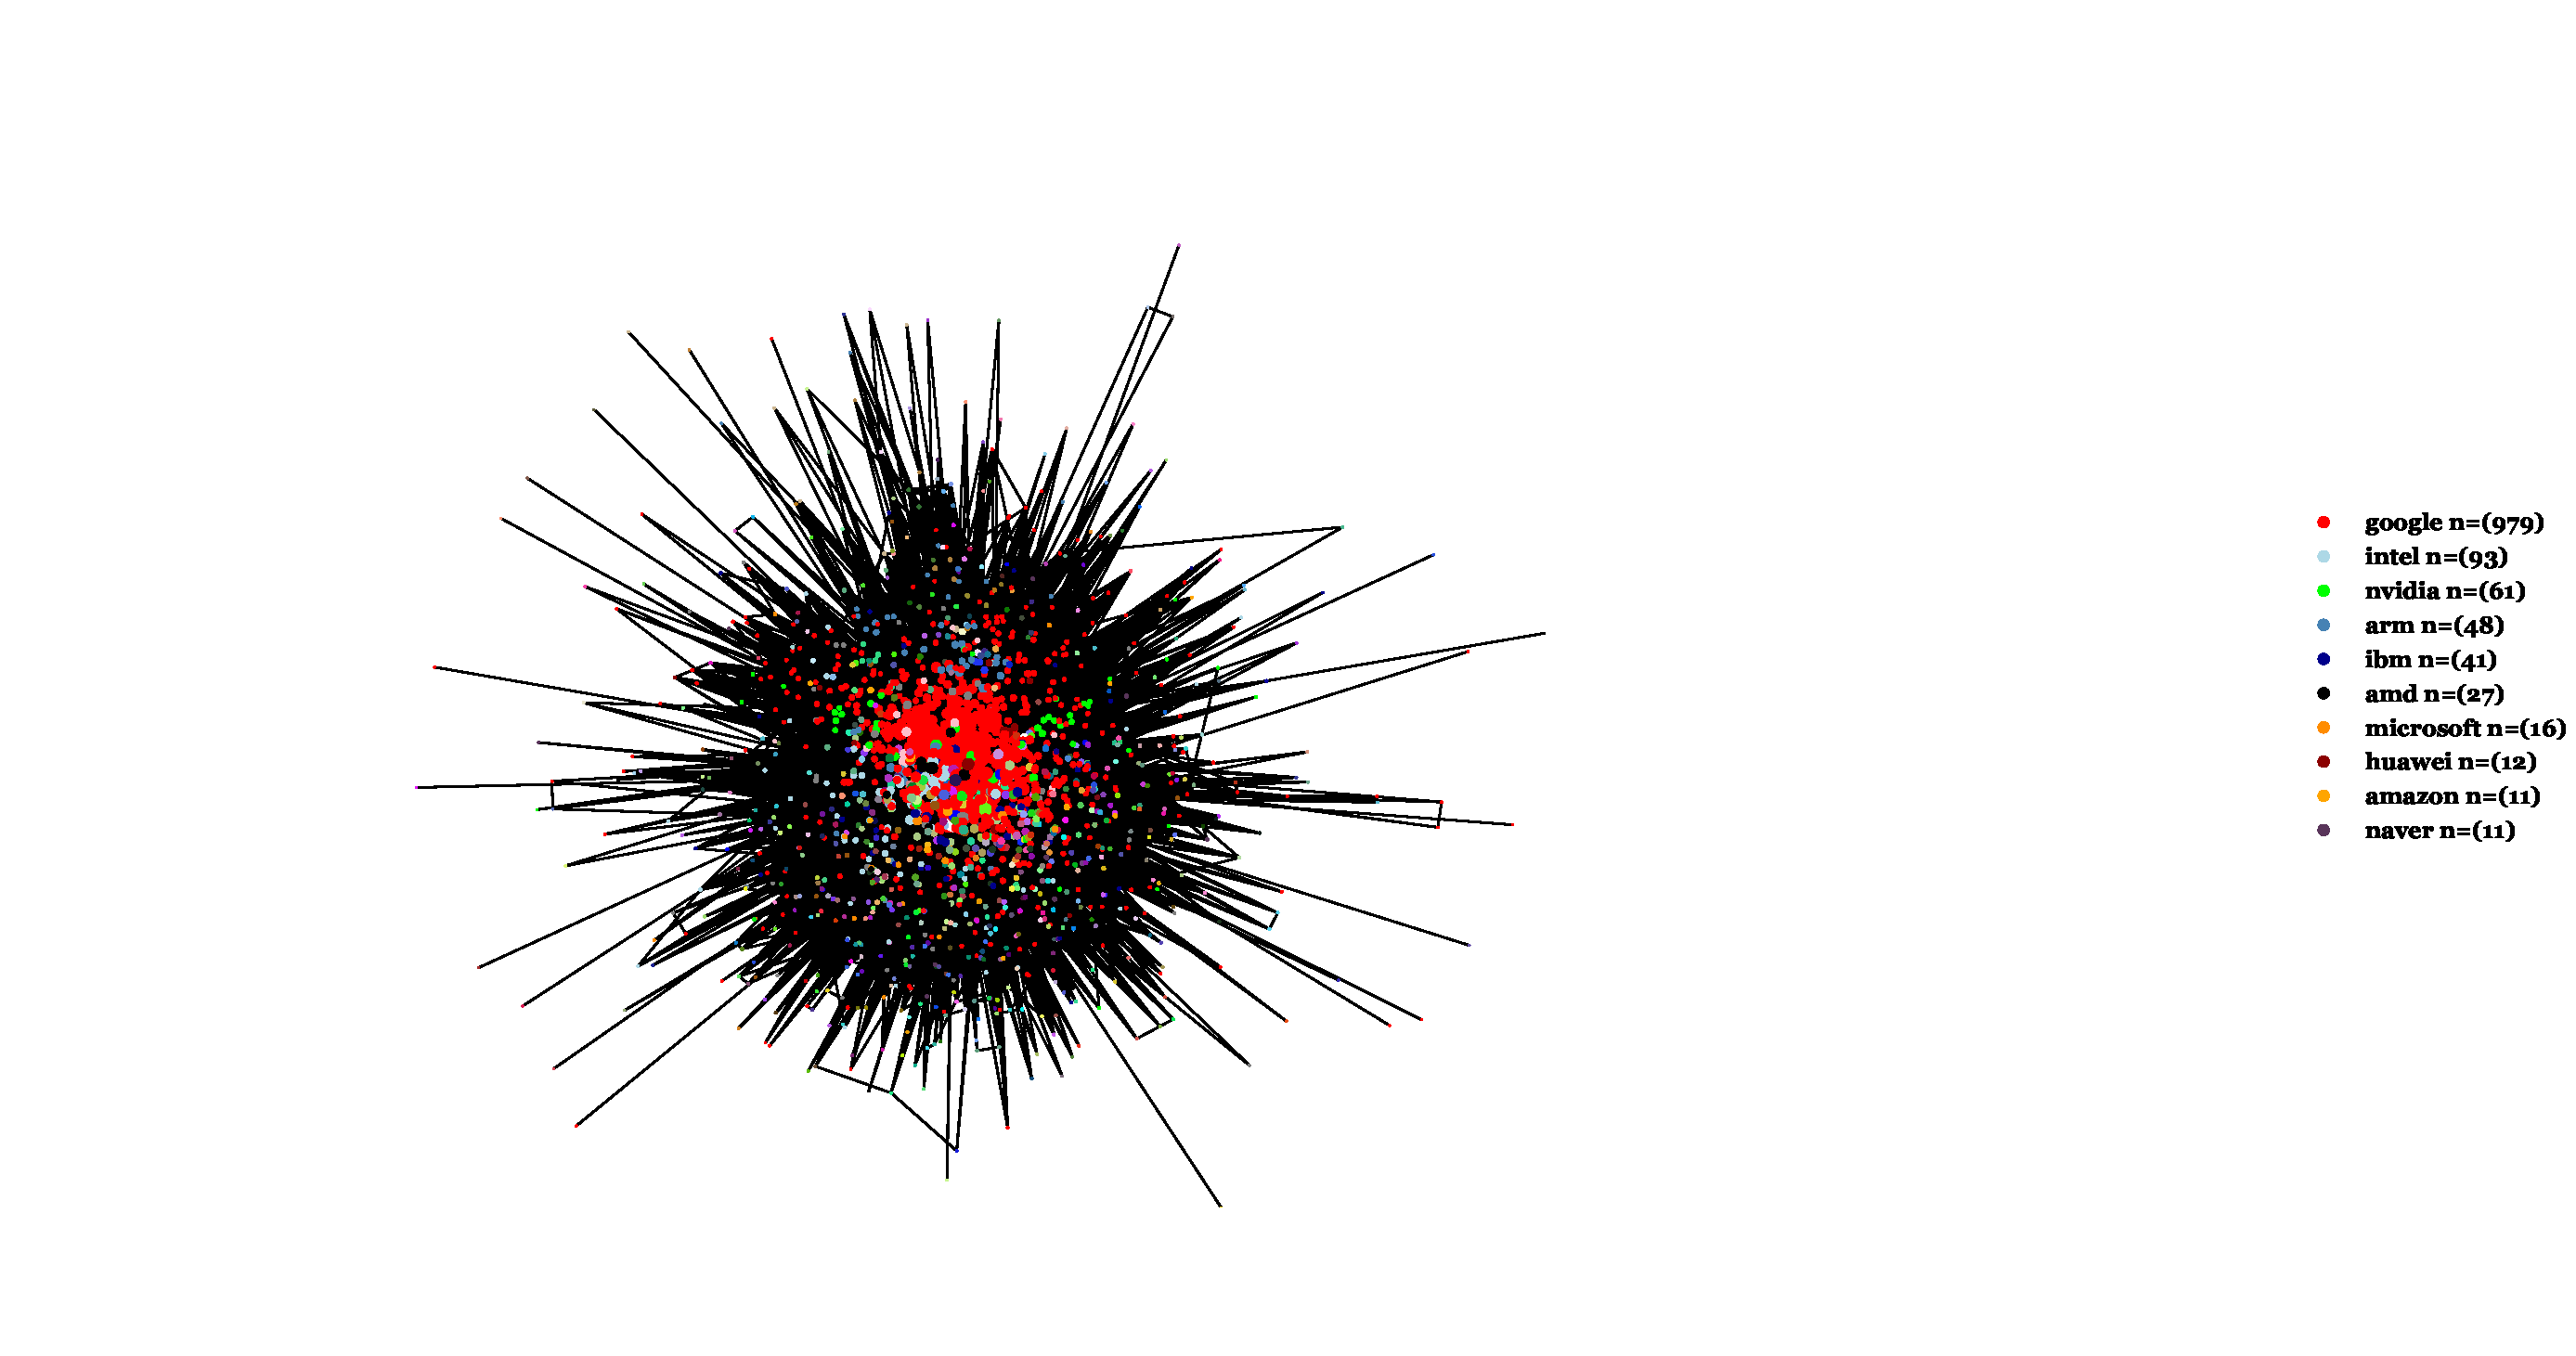
\includegraphics[draft=false,
keepaspectratio=true,width=0.9\textwidth,trim={0 1cm 0 2cm},clip]{Figures/all.pdf}
 % TensorFlowGitLog-2015-git-log-outpuyt-by-Jose.IN.NetworkFile.graphMLUncolored-Centrality-Layout.png: 640x480 px, 100dpi, 16.26x12.19 cm, bb=0 0 461 346
 \caption{Sociogram capturing collaboration among developers during Nov 2014 - Apr 2024.}
 \label{figall}
\end{figure}
}





\subsubsection{Pointing our lenses to SNU}




% Generated by 5-add-code-to-main.tex.sh 
\iftoggle{TaFigOnEnd}{
\InsertHere{Figure}{Scrap log output for SNU.}{\ref{figSNU}}{10}
}
{
\begin{figure}[h]
\centering
\includegraphics[keepaspectratio=true,width=0.9\textwidth]{./Figures/noo/SNU_cropped.pdf}
\caption{Scrap log output for SNU.\label{figSNU}}
\end{figure}
}


Our first figure capturing  inter-organizational network cooperation at an aggregated level (see \Cref{figSNU}), showcases relationships and interactions between SNU and the top ten contributors to the TensorFlow platform for \ac{AI} and \ac{ML} (i.e., Google, Intel, Nvidia,, , ARM, IBM, AMD, Microsoft, Huawei, Amazon and Naver).
Nodes in the network represent organizations, while edges (lines connecting the nodes) indicate the existence and strength of collaborative ties between them. The size of the nodes reflect the centrality and prominence of the organizations and the edges  represent the intensity and  frequency of collaborative interactions in the co-production of the TensorFlow  software source code. Each node's label maps the organization name, and each edges's label represent the number of unique collaborations among software developers affiliated with the organizations the edge connects. In other words, the high the edge's label number, the more developers affiliated with the organizations cooperated with each other. For example, Huawei and SNU had six unique inter-organizational collaborative relationships among software developers, while IBM and SNU had 16 developers\footnote{Note that as SNU has 7 individual contributors and Huawei has 12 individual contributors, there is a maximum of $7x12=84$ possible inter-organizational relationship combinations involving both SNU and Huawei developers. However, as Google had  979 nodes,  there is a maximum of 6853 possible combinations involving both SNU and Google developers.}


As noted in \Cref{figSNU}, Google is the most central node as expected by being the founder, and biggest investor on TensorFlow. Following in terms of centrality, we note that chipset makers (i.e., Intel, ARM, Nvidia and Nvidia) and cloud vendors (Amazon, IBM and Microsoft) form central core of the TensorFlow collaborative network. SNU as University contributor remain in the periphery with strong ties with Google, Intel, AMD, IBM and Nvidia and weaker ties with Naver and Microsoft.  Somehow surprising (as both Naver and SNU are Korean organizations), both organizations only had on inter-organizational collaborative dyad.  The network also provides insights into strategic alliances where companies like AMD and Nvidia, despite being competitors, engage recurrent collaborative efforts. The fact that they sell competing cloud services or products or competing chipset do not reflect on the collaborative network. The collaborative network do not shows evidence that competition in the chipset and cloud computing market influences cooperation in the TensorFlow ecosystem. 

On the one direction, and besides being in the network periphery (see  \Cref{figSNU}), SNU plays a very important bridge role in the network. SNU acts as bridge to (1) researchers with high high-level expertise in developing and deploying \ac{ML} learning models,  (2) as a bridge to talent that is recruited by the organizations that develop and deploy TensorFlow, and (3)
as a bridge between theoretical research and practical real-world applications.



On the other hand, by  contributing to TensorFlow, SNU researchers can stay at the forefront of AI and \ac{ML} research and  access to the world-class cloud infrastructure maintained by Google. Furthermore, by contributing to TensorFlow, SNU can incorporate the latest \ac{AI} and \ac{ML} technologies into its curriculum, providing students with hands-on experience and preparing them for careers in \ac{AI} and \ac{ML}. As many researchers seek societal impact,by contributing to TensorFlow, researchers can see their model, their code and their algorithms applied to a vast cross-industrial domain that ranges from healthcare, telecommunications, automotive, social networks and robotics. By contributing to its development.  While advances on TensorFlow  immediately impact  natural language processing, computer vision, and automated machine learning, those advancements can benefit society at large (better translations, self-driving cars, better hand-writing recognition, better diagnostics, automation of boring or dangerous tasks thus, leading to advancements that benefit society at large. Contributions to a widely-used and respected framework like TensorFlow and a strong partnership with Google and other big players in the ecosystem enhance SNU's reputation in the global research community, attracting funding, partnerships, and top-tier faculty and students. In summary, SNU's contributions to TensorFlow stem from a desire to advance research and access the required infrastructure, foster collaboration, enhance educational programs, create societal impact, and bolster institutional recognition. These efforts align with the university's goals of driving innovation and maintaining a leadership position in the fields of \ac{AI} and \ac{ML}.

\subsection{Pointing our lenses to DFKI}


\iftoggle{TaFigOnEnd}{
\InsertHere{Figure}{Scraplog output for dfki.}{\ref{figdfki}}{10}
}
{
% Generated by 5-add-code-to-main.tex.sh 
\begin{figure}[h]
\centering
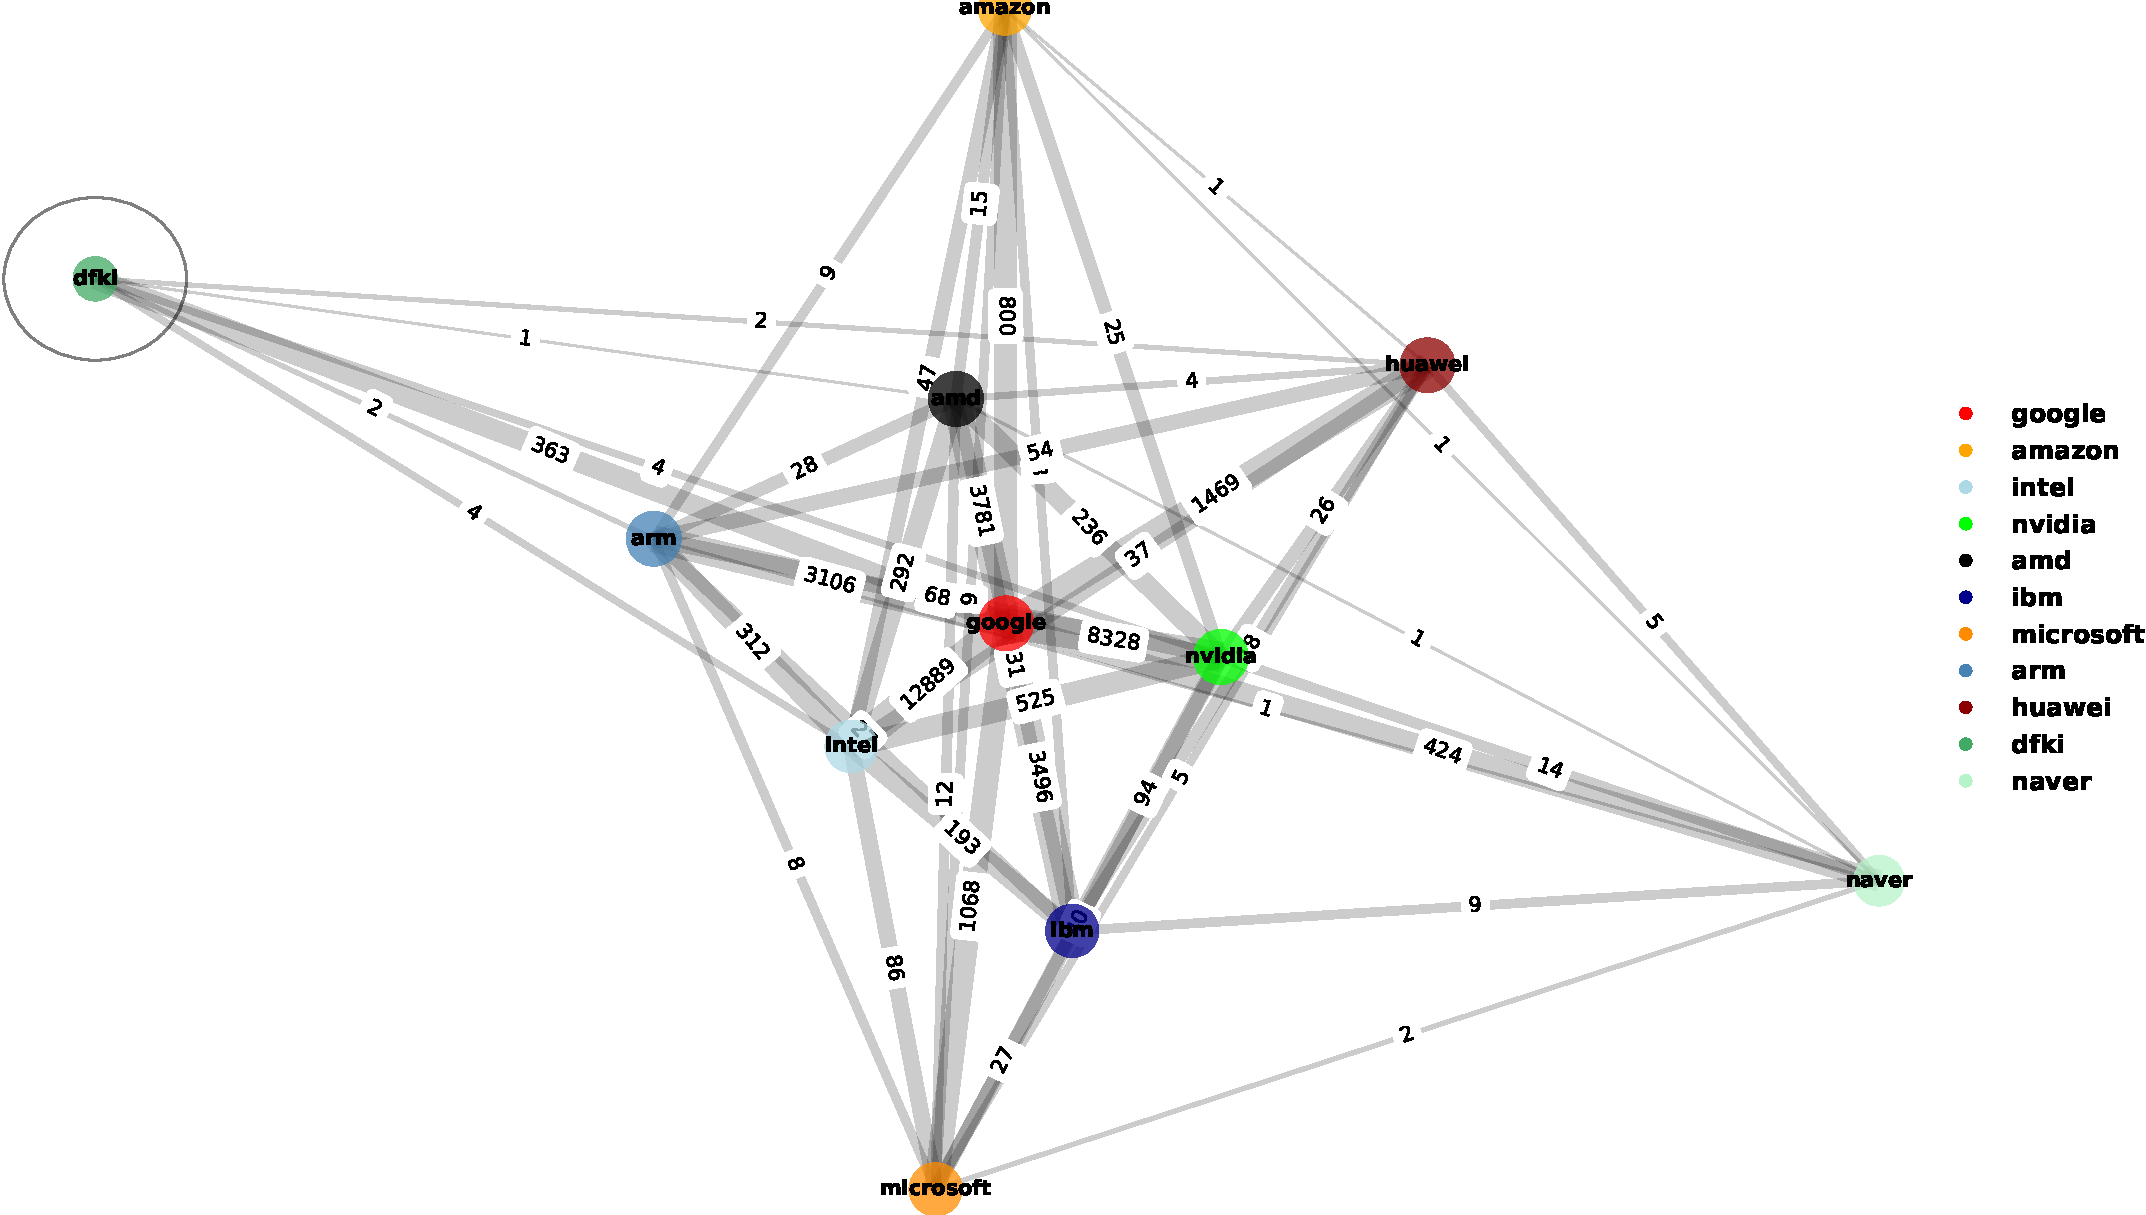
\includegraphics[keepaspectratio=true,width=0.9\textwidth]{./Figures/noo/dfki_cropped.pdf}
\caption{Scraplog output for dfki.}
\label{figdfki}
\end{figure}
}


Our second figure capturing  inter-organizational network cooperation at an aggregated level (see \Cref{figdfki}), showcases relationships and interactions between DFKI and the top ten contributors to the TensorFlow platform  in the same fashion as in \Cref{figSNU}.  Nodes represent organizations and edges represent collaboration as in the same way. Each node's is labeled with its organization name, and each edge is labeled with the  number of unique collaborations among software developers affiliated with the organizations that the edge connects. In other words, the high the edge's label number, the more developers affiliated with the two nodes cooperated with each other. 

DFKI as research institute contributor remain in the periphery with a unique strong tie with Google and  weaker ties with Huawei, Nvidia, AMD, Intel and ARM.  Somehow surprising ( DFKI as a German research institute does not collaborate more with organizations that have large offices in Germany). The contributions of DFKI seem to be coupled with chipset design given that DFKI works with most of the chipset vendors but not with the most well know provider of cloud services (e.g., Amazon, IBM, and Microsoft).




On the one direction, and besides being in the network periphery (see  \Cref{figdfki}), DFKI also plays a very important bridge role in the network. DFKI  also acts as bridge to (1) researchers with high high-level expertise in developing and deploying machine learning models,  (2) as a bridge to talent that is recruited by the organizations that develop and deploy TensorFlow, and (3) as a bridge between theoretical research and practical real-world applications. In the case of DFKI, our qualitative part of the investigation (i.e., interview with developers) highlight that DFKI cross-fertilized theoretical and practical competences in sector that are particularity important for the German economy (e.g., automotive, healthcare and manufacturing of precision machinery). This might explain why DFKI worker closer to chipset makers than to cloud vendors. 


DFKI, along with its partners, secured funding from the European Union's Horizon 2020 program for projects that involve the development and application of AI technologies using TensorFlow. 
Funding from German national research agencies, such as the Federal Ministry of Education and Research (BMBF), has been utilized to support collaborative projects between DFKI and industry partners like Google. These funds supported research activities, including the hiring of researchers, purchasing of equipment, and running computational experiments. And were often done in collaboration with industrial partners that early jumped into testing and adopting \ac{AI} and \ac{ML} into their operations (e.g., OEM car-makers, hospital diagnostics centres).
 Without Google, it would be hard for DFKI and its partners to have ready to deploy high-performance computing (HPC) facilities for running large-scale machine learning experiments and training complex models using TensorFlow.


\subsection{Pointing our lenses to Chromium}

The third non-commercial organization with the most contributors to TensorFlow is not a University nor a Research Institute. To our surprise, it was instead the Chromium open-source community which is an open-source project primarily maintained and managed by Google. The project started using the WebKit rendering engine\footnote{See the work of \citet{TeixeiraLin2014} on WebKit that coined the term open-coopetition.}. When Google first launched Chromium and its commercial counterpart, Google Chrome, in 2008, they used WebKit as the browser's rendering engine. WebKit, initially developed by Apple for its Safari browser, was chosen due to its performance and compatibility.

However, in 2013, Google decided to create a separate fork of WebKit called Blink. This decision was driven by the desire to have more control over the development process and to innovate more rapidly without being tied to WebKit's development constraints and priorities. Blink allowed Google to make significant changes and optimizations specific to the Chromium project, leading to enhancements in performance, security, and compatibility.

The transition from WebKit to Blink marked a significant evolution in the Chromium project, allowing Google and other contributors to push the boundaries of what web browsers could achieve. Today, Blink is the rendering engine behind not only Google Chrome but also other Chromium-based browsers like Microsoft Edge, Opera, and Brave. Chromium serves as the foundational codebase for Google Chrome and several other web browsers, including Microsoft Edge, Brave, Opera, and Vivaldi. As an open-source project, Chromium invites contributions from developers worldwide, allowing for a diverse range of inputs and innovations. Google directs the overall development and ensures that contributions align with the project's goals and standards, but the open-source nature of Chromium means that it benefits from a wide array of perspectives and expertise, driving continuous improvement and adaptability.

The Chromium project operates under the permissive BSD license, which allows anyone to use, modify, and distribute the code. This licensing structure has enabled various companies and developers to build upon the Chromium codebase, integrating unique features and optimizations to cater to different user needs. For instance, Google Chrome includes proprietary enhancements and services on top of Chromium, while Microsoft Edge incorporates its features and integrations. The Chromium open-source community plays a crucial role in identifying bugs, proposing enhancements, and ensuring the project's security and stability. 

It is important to notice that even if Google has significant control over the Chromium project as its primary maintainer, it cannot unilaterally close Chromium in the traditional sense of making it proprietary and removing access to the existing open-source code. Once code is released under the BSD license, those rights cannot be revoked for the code that has already been released. Furthermore, Chromium integrates large components of open-source code released under permissive copyleft licenses that would need to be rewritten at very high costs if Google chose to move the project from the open-source to the proprietary arena.  Finally, if Google were to cease its open-source development of Chromium or attempt to close it, the community or other organizations could fork the project \citep[see][for academic discussions on the implications of the forking mechanism]{KarhuGustafsson_et_al2018,NymanLindman2013}. This means they could take the existing open-source code and continue development independently of Google under a different name.  Closing Chromium could alienate the developer community and other stakeholders who contribute to the project, ultimately harming Google’s interests.


By interviewing at developer that did not wish to reveal its identity, Google employs developers with @chromium.org email addresses to distinguish their contributions to the Chromium project from other Google-related activities. This practice serves several important purposes such as: (1) ensuring that contributions are correctly attributed to the open-source project rather than other Google initiatives. 
Clear Project Identification, (2)  maintaining transparency within the open-source community,  By having a distinct email domain, it is clear which contributions are made on behalf of Chromium even if by developers paid by Google, (3) create a sense of community and shared purpose among contributors, whether they are from Google or other organizations. Google developers may work on various projects simultaneously, however  having a separate email domain for Chromium helps to differentiate communications and commitments specific to the Chromium project are managed distinctly from other Google projects.








% Licenses force open-coopetiton 


\iftoggle{TaFigOnEnd}{
\InsertHere{Figure}{Scraplog output for chromium.}{\ref{fig:chromium}}{10}
}
{
% Generated by 5-add-code-to-main.tex.sh 
\begin{figure}[h]
\centering
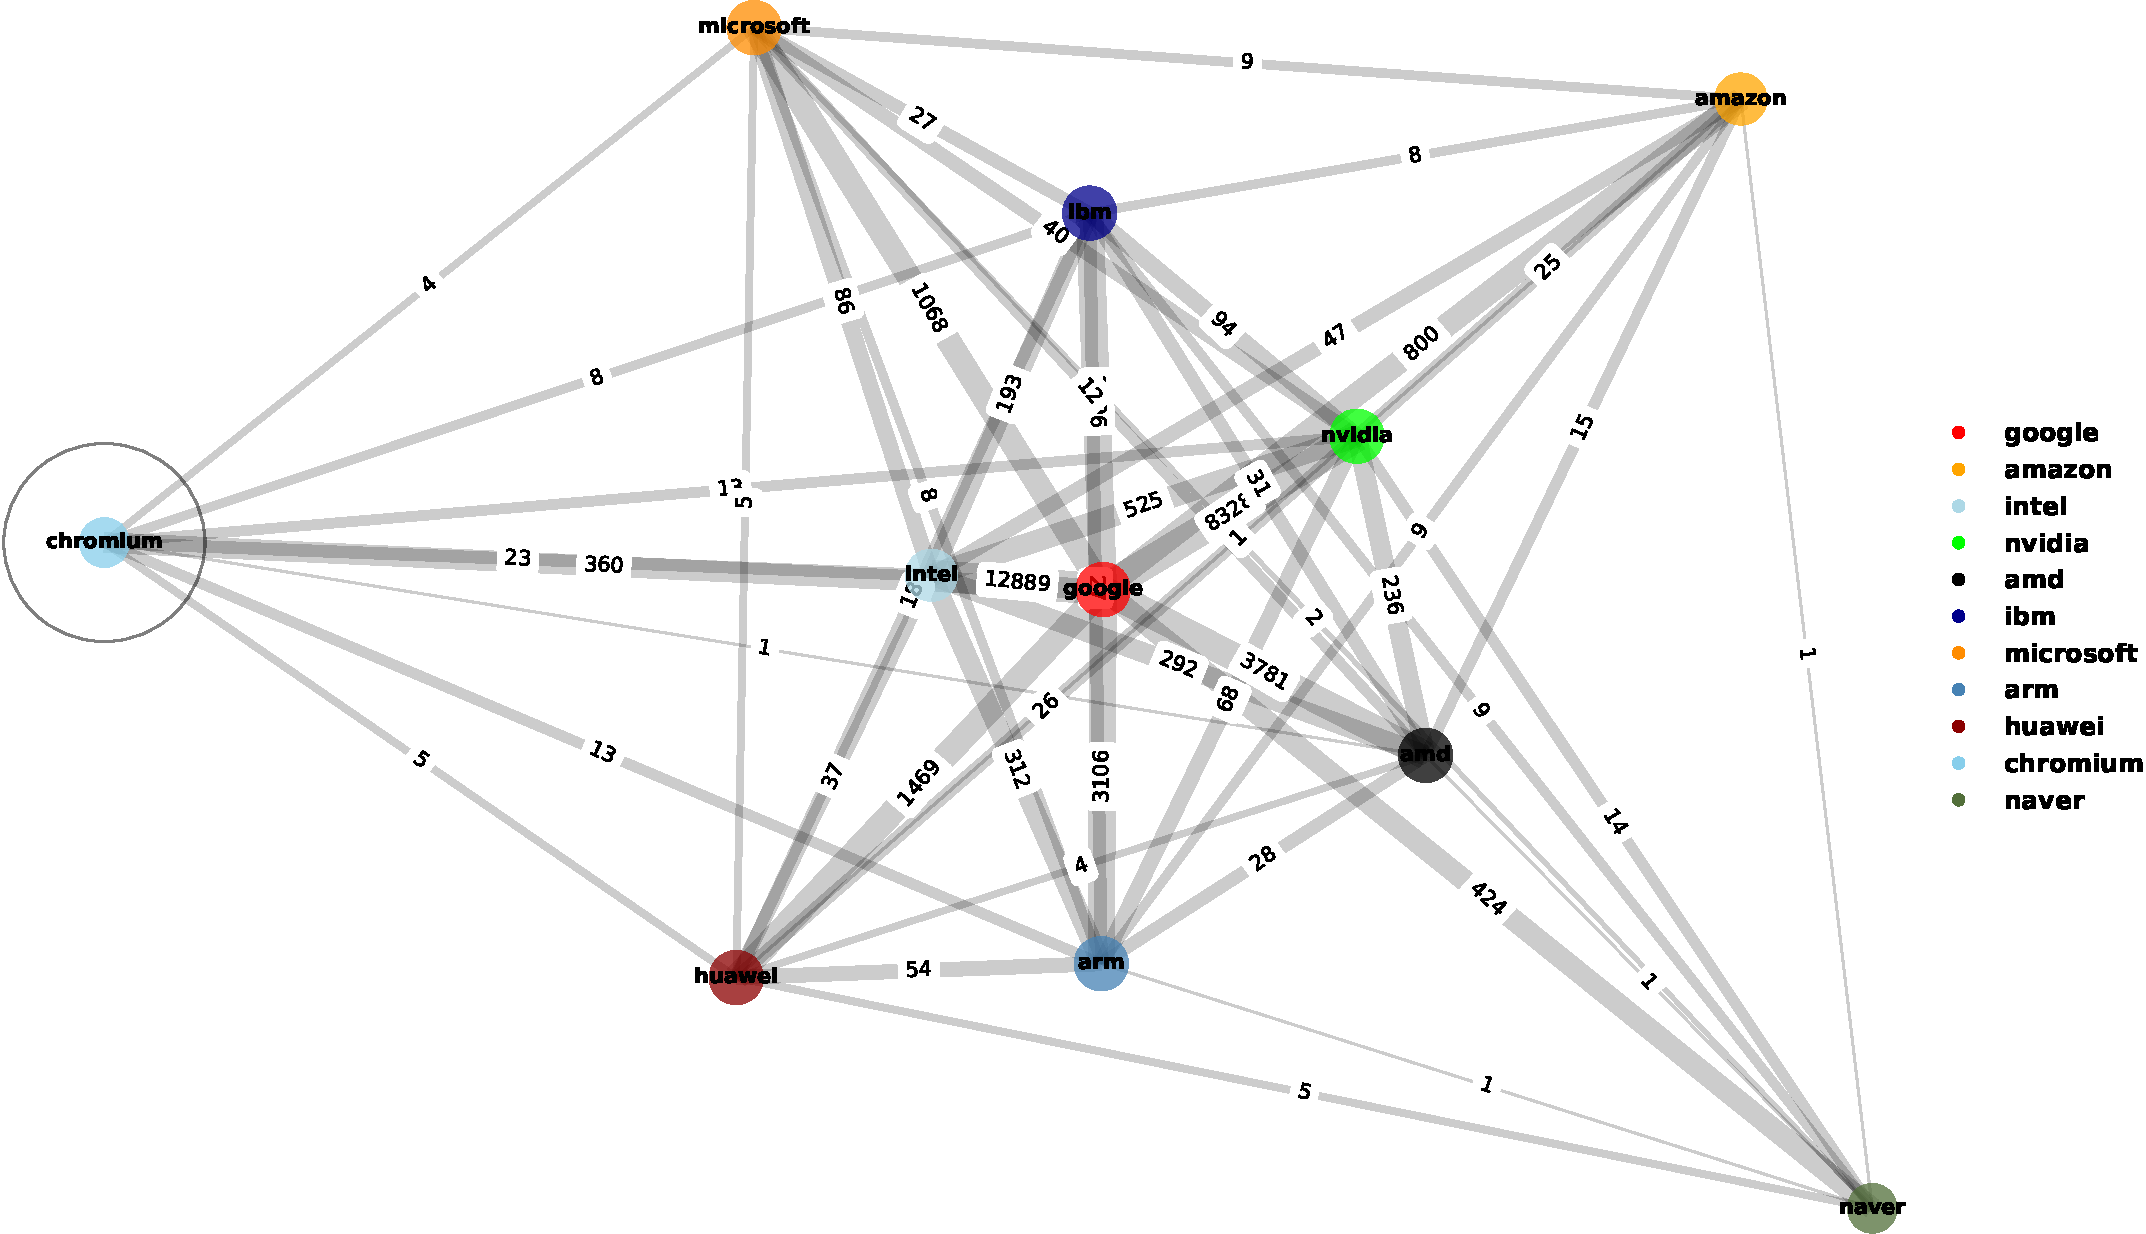
\includegraphics[keepaspectratio=true,width=0.9\textwidth]{./Figures/noo/chromium_cropped.pdf}
\caption{Scraplog output for chromium}
\label{fig:chromium}
\end{figure}
}



The Chromium project, although primarily maintained by Google, aims to present itself as a neutral platform for browser development. This neutrality allows it to attract contributions from other major tech companies like Microsoft (for Edge), Opera, and Brave. By fostering an inclusive and collaborative environment, Chromium can benefit from a wide range of expertise and innovations, driving the project forward and ensuring its continued relevance and success.
In line with other open-source communities like the ones represented by Linux Foundation, the Apache Foundation, and the Eclipse Foundation \citep[see][for work on conflict of interest in open-source foundations]{weikert2019managing}, the Chromium project needs to be a neutral space where competitors can collaborate.  Therefore organizations like the Chromium project play a very important dual role (1) maintain a software code base in an open-source way that for several reasons can not be turned into commercial software, and (2) be a neutral place that ensures openness and transparency in the orchestration of collective goals as evidenced by the following quote that pop-up during one semi-structured interview with a TensorFlow developer recruited via e-mail and LinkedIn.  

\begin{quotation}
``A neutral governance model ensures that everyone can contribute and benefit equally, which is essential for the health and growth of the project'' ... `` there needs to be a neutral space for competitors to push code''  -- Software developer  and regular contributors to the TensorFlow during a semi-structured interview with the first author.  Pseudonym Albert. 
\end{quotation}


While SNU and DFKI roles on the network were more about bridging competence, the role of Chromium was more about bridging with an established open-source code base and bridging with a neutral space where organizations with competing interests work together. 


\subsection{Pointing our lenses to ISP}


Also to our surprise, the fourth non-commercial organization that most contributes to TensorFlow code was the Institute for System Programming of the Russian Academy of Sciences (ISP). Also 
very far away from California, ISP  contributed to TensorFlow, particularly in areas related to software verification and formal methods. Their contributions have primarily focused on enhancing the reliability and correctness of TensorFlow's codebase.

The ISP is a research institution focused on advanced software development and system programming. Founded in 1994, the ISP RAS engages in extensive research and development in areas such as formal methods, system programming, software verification, and programming languages. The institute collaborates with both domestic and international organizations, contributing significantly to the global software development community. The research institute has also a portfolio of open-source projects in the areas of  software verification, physical dynamics simulators, functional verification of microprocessors and natural language processing. Their contributions to TensorFlow are another showcase of their advanced competencies on the international stage. 


Our  \Cref{figispras} captures inter-organizational network cooperation  between 
 ISP and the top ten organizational commercial companies that co-produce TensorFlow show that ISP as research institute organizational contributor remains in the periphery with strong ties with Google followed by ARM and Intel and weaker ties with  Nvidia, Huawei, IBM and Naver.  The contributions of ISP seem to be coupled with the chipset design makers.  In the same way as DFKI, ISP works the most with Google and the chipset vendors but not so much with the most well-known providers of cloud services (e.g., Amazon, IBM, and Microsoft).



\iftoggle{TaFigOnEnd}{
\InsertHere{Figure}{Scraplog output for ispras.}{\ref{figispras}}{10}
}
{
% Generated by 5-add-code-to-main.tex.sh 
\begin{figure}[h]
\centering
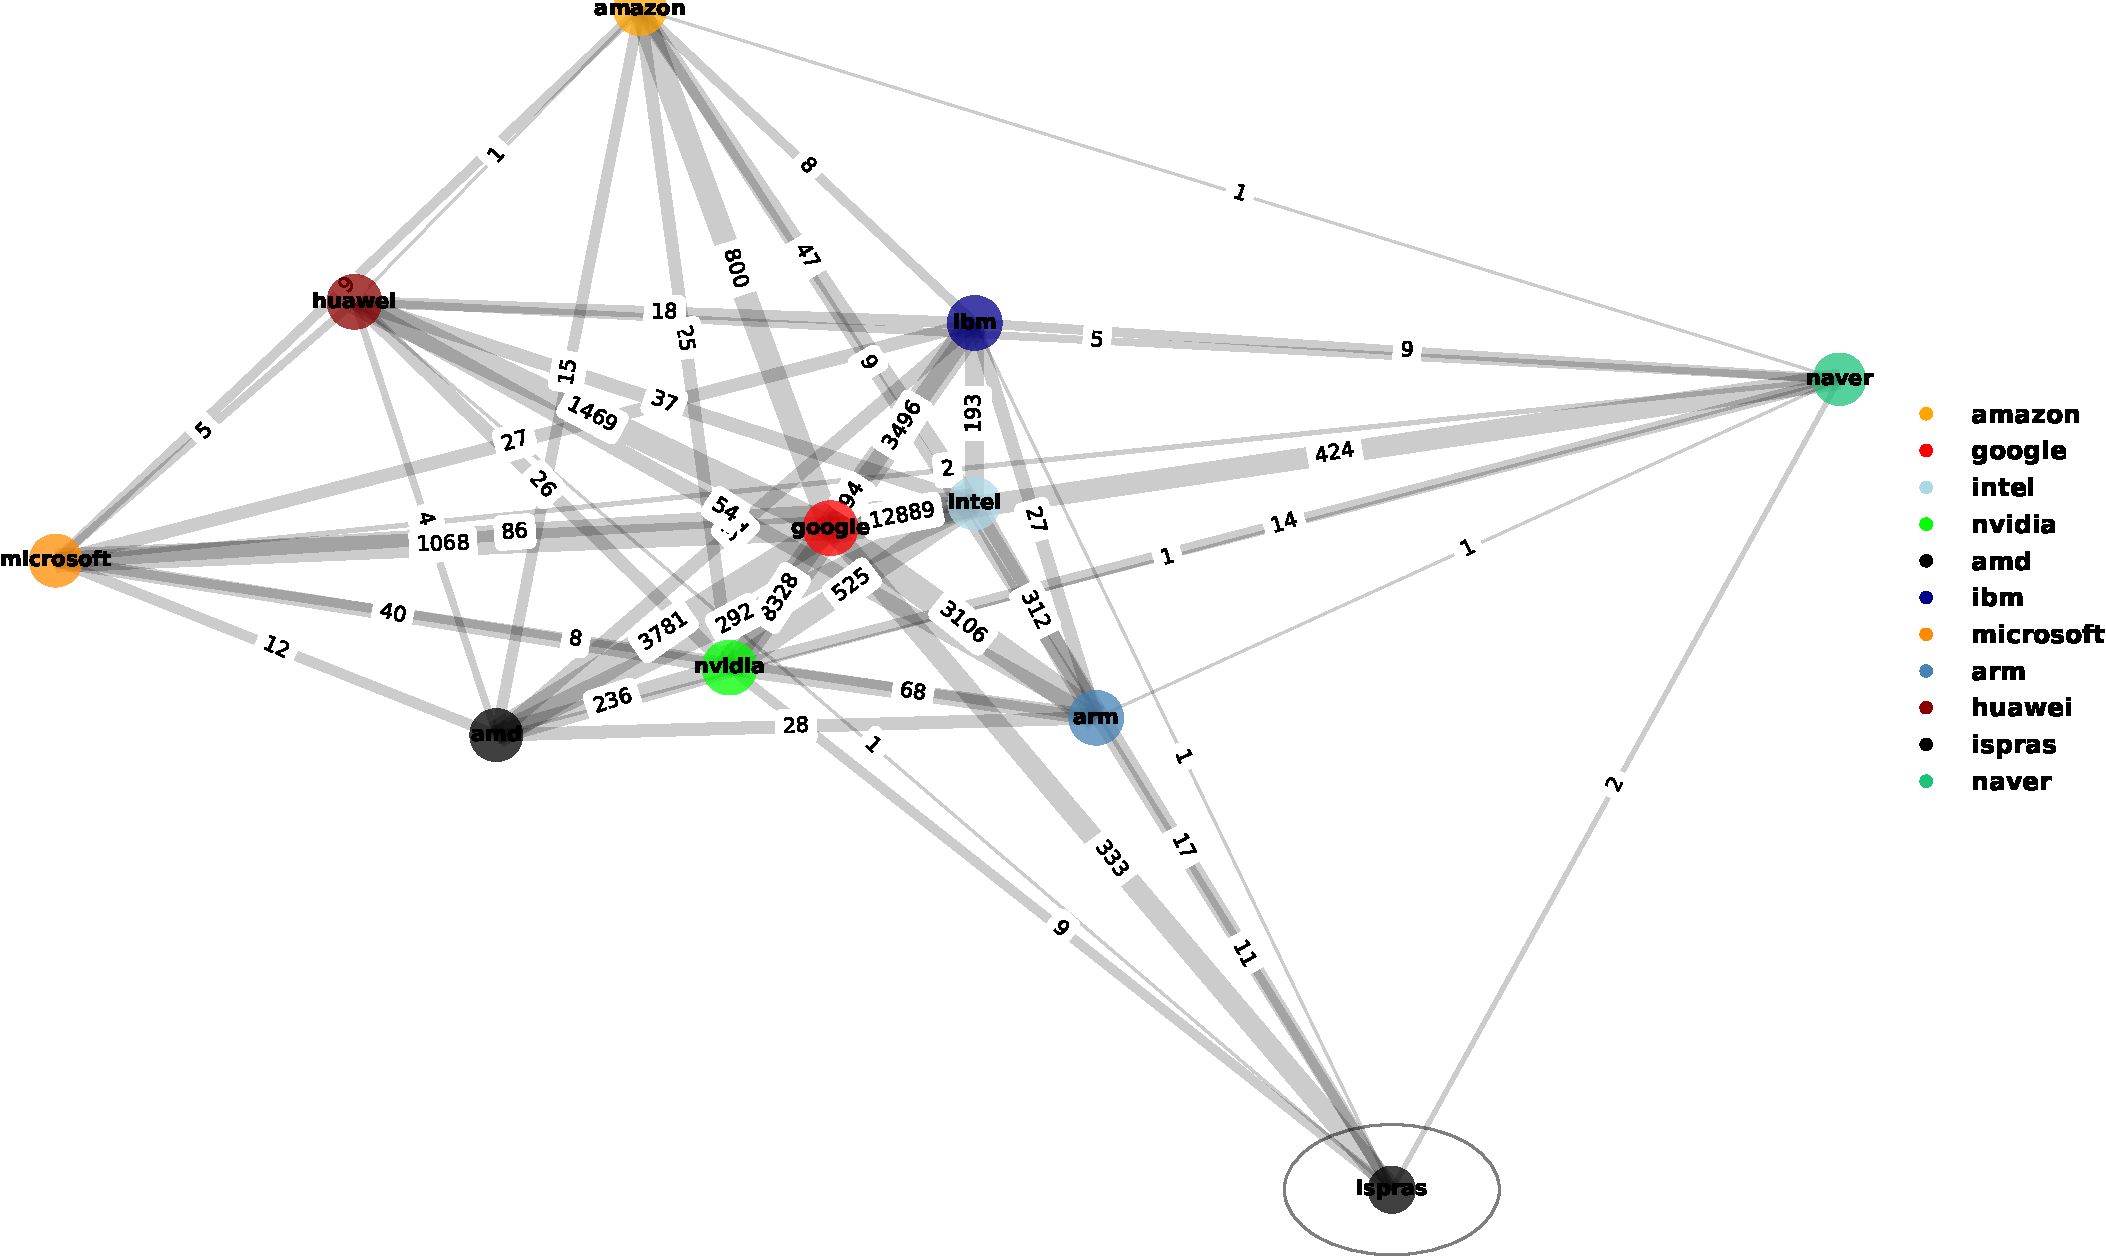
\includegraphics[keepaspectratio=true,width=0.9\textwidth]{./Figures/noo/ispras_cropped.pdf}
\caption{Scraplog output for ispras}
\label{figispras}
\end{figure}
}


From the one side, Google and its TensorFlow partners benefited from the ISP static analysis and verification tools for TensorFlow that were designed to identify and correct bugs, improve code safety, and ensure compliance with coding standards in the project. Furthermore, the ISP also provided tools and services for the formal verification of TensorFlow's algorithms. A difficult task in computer science that involves creating mathematical models of the algorithms and proving their correctness and robustness.

On the other side, the collaboration provided ISP RAS with access to Google's computational resources and development environments. This access enabled them to perform extensive testing and verification processes, which would be challenging to achieve independently. The joint efforts likely resulted in academic publications, conference presentations, and technical reports that contribute to the broader research community. These outputs disseminate knowledge, promote best practices in software verification, and showcase the ISP tools and methodologies in the growing \ac{AI} industry.

\subsection{Pointing our lenses to PKU}



% Who are they 

The fifth non-commercial organization that most contributes to the TensorFlow code was Peking  University (PKU). Like SNU, PKU us a University located quite far from California where the TensorFlow project was born. Both PKU and SNU are (1) top academic institutions in their own countries, (2) rank high in the international ranking organizations, (3) host many research institutes and centres, and (4) develop international partnerships with the industry on the global stage. In this sense, in terms of industry-university relations, we should not only see those universities as Korean or Chinese, but as ``world'' universities. The same applies to other universities and research institutes that contribute to TensorFlow listed in \Cref{tnoncomercial}. 


The PKU  hosts the Institute for Artificial Intelligence that was established in April 2019and  hosts itself dozens AI labs  with different expertise (e.g., healthcare, cognitive reasoning, and image recognition among others). PKU established multiple formal partnerships with Huawei and many Europeans and North American organizations when it comes to \ac{AI} and \ac{ML} (e.g., UCLA-PKU Joint Research Institute in Science and Engineering (JRI) or the ). By retrieving online documentation and speaking to TensorFlow developers we were surprised by the fact that 
Huawei, in collaboration with PKU, has developed its own \ac{GPUs}, called the Ascend series that is very competitive for \ac{AI} and \ac{ML} workloads making the Chinese AI industry less dependent on USA chipsets\footnote{ See \href{https://www.tomshardware.com/news/huaweis-gpu-reportedly-matches-Nvidias-a100-report}{https://www.tomshardware.com/news/huaweis-gpu-reportedly-matches-Nvidias-a100-report}.}. While Chinese tech giants like Alibaba, Tencent, and Baidu are reportedly turning to Huawei for \ac{GPUs}, Huawei has also been developing its \ac{AI} accelerator chips, which are similar to Google's \ac{TPUs}.


In \Cref{figpku}, we capture inter-organizational network cooperation  between 
PKU and the top ten organizational commercial companies that co-produce TensorFlow show that ISP as a research institute organizational contributor remains in the periphery with a very strong tie with Google. Then PKU has weak ties with Huawei, Nvidia, and Naver. The multiple formal partnerships between Huawei and PKU are not be strongly visible in the TensorFlow code repository, as only two dyads of developers established an inter-organisational collaboration relationship between PKU and Huawei (see left side of \Cref{figpku}). This suggests that the cooperation between PKU and Huawei in terms of advancing \ac{AI}, \ac{ML} happens somewhere else than in the TensorFlow core. 




% What the figure shows 

% Question 1 ,2, 3 an 4 

\iftoggle{TaFigOnEnd}{
\InsertHere{Figure}{Scraplog output for pku.}{\ref{figpku}}{10}
}
{
% Generated by 5-add-code-to-main.tex.sh 
\begin{figure}[h]
\centering
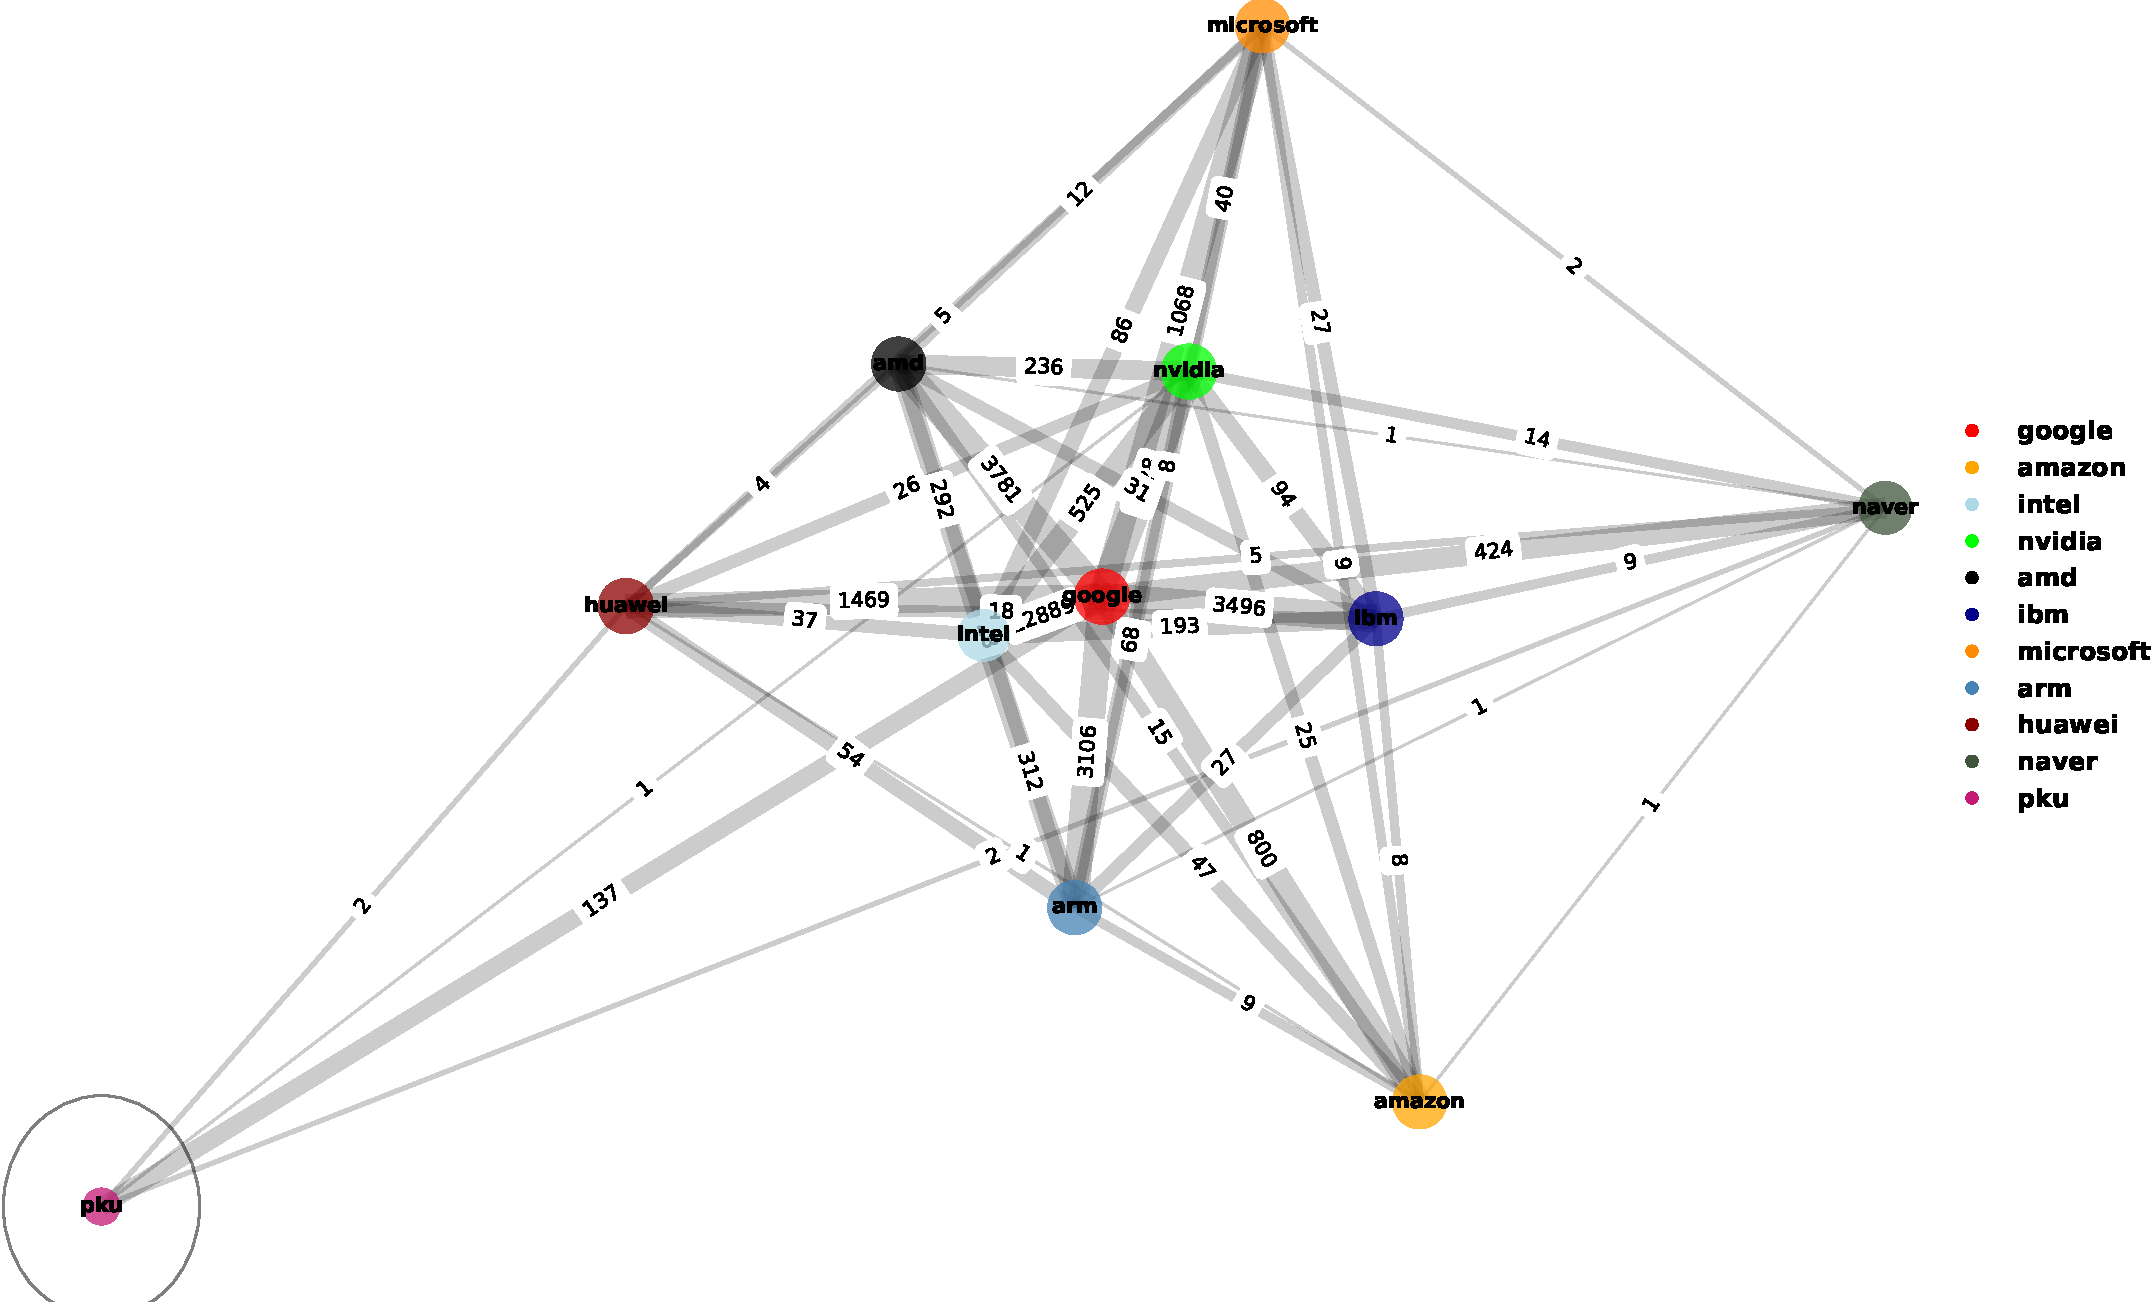
\includegraphics[keepaspectratio=true,width=0.9\textwidth]{./Figures/noo/pku_cropped.pdf}
\caption{Scraplog output for pku}
\label{figpku}
\end{figure}
}


Significant contributions from PKU include research on Semantic Image Segmentation which involves detailed work on improving the accuracy and efficiency of semantic segmentation models. This project has seen contributions from both Google and academic researchers, including those from PKU, focusing on enhancing convolutional neural networks (CNNs) and developing new methods for object localization in images​. Another example is the ``Show and Tell'' image captioning system, where researchers from both organizations worked on improving the computer vision components of TensorFlow to generate more detailed and accurate image descriptions. This collaboration not only resulted in advancements in image captioning techniques but also provided extensive open-source in the form of code to TensorFlow.  PKU seems to act as a bridge to competence in computer image recognition that in the last years been improving a lot with the advance of \ac{AI} and \ac{ML}.

From the perspective of PKU, our analysis points out four motivations for its engagement in the co-production of TensorFlow. First, in terms of research and innovation, PKU's participation in TensorFlow allows its researchers to pursue cutting-edge AI and machine learning research, enhancing the university's academic and scientific capabilities. Collaborating with industry leaders like Google augments PKU's research output and contributes to the advancement of state-of-the-art technologies. Second, and in terms of access to resources and expertise, collaborating on TensorFlow provides PKU with access to Google's extensive resources, including computational infrastructure and expert knowledge in AI and machine learning. This partnership enables PKU researchers to work on large-scale projects and leverage Google's experience to enhance their own research and development efforts. Thirds, and in terms of educational impact, PKU's contributions to TensorFlow have significant educational benefits as PKU created educational resources, such as TensorFlow tutorials and courses, which help train the next generation of \ac{AI} and \ac{ML} researchers and practitioners. Finally, in terms of reputation, by participating in high-profile open-source projects like TensorFlow, PKU strengthens its global reputation and fosters international collaborations.
Overall, PKU's involvement in the co-production of TensorFlow is driven by its desire to advance research, gain access to valuable resources that would be harder to fulfil by itself, enhance educational offerings, and solidify its position as a leader in the \ac{AI} and \ac{ML} landscape.

\subsection{Pointing our lenses to GeorgiaTech}


The sixth non-commercial organization that most contributes to the TensorFlow code is the North American Georgia Institute of Technology which is commonly known as GeorgiaTech.  As visible \Cref{figgatech}, GeorgiaTech similar to all other non-commercial players listed \Cref{tnoncomercial} has a strong tie with Google.  Besides the strong tie with Google, GeorgiaTech also has weaker ties with Nvidia (USA-based) and Huawei (China-based). For the later inter-organizational relationship, we could only find one pair of developers collaborating across the organizations. 


Georgia Tech has been actively involved in projects that leverage the TensorFlow platform for\ac{AI} and \ac{ML}  research. These projects often involve interdisciplinary collaborations, such as the work conducted by the Interactive Media Technology Center, which explores the usability and applications of wearable computing interfaces in assistive technologies. Georgia Tech's extensive research infrastructure and computing resources have been instrumental in supporting TensorFlow-related projects. This includes utilizing high-performance computing clusters and specialized facilities like the GT-Bionics Lab, which focuses on developing assistive technologies to empower individuals with severe disabilities. In some cases, Georgia Tech has established industrial partnerships in the domains of AI and machine learning, which have helped secure research and development funding and bridge the gap between academic research and practical, real-world applications.





\iftoggle{TaFigOnEnd}{
\InsertHere{Figure}{Scraplog output for gatech.}{\ref{figgatech}}{10}
}
{
% Generated by 5-add-code-to-main.tex.sh 
\begin{figure}[h]
\centering
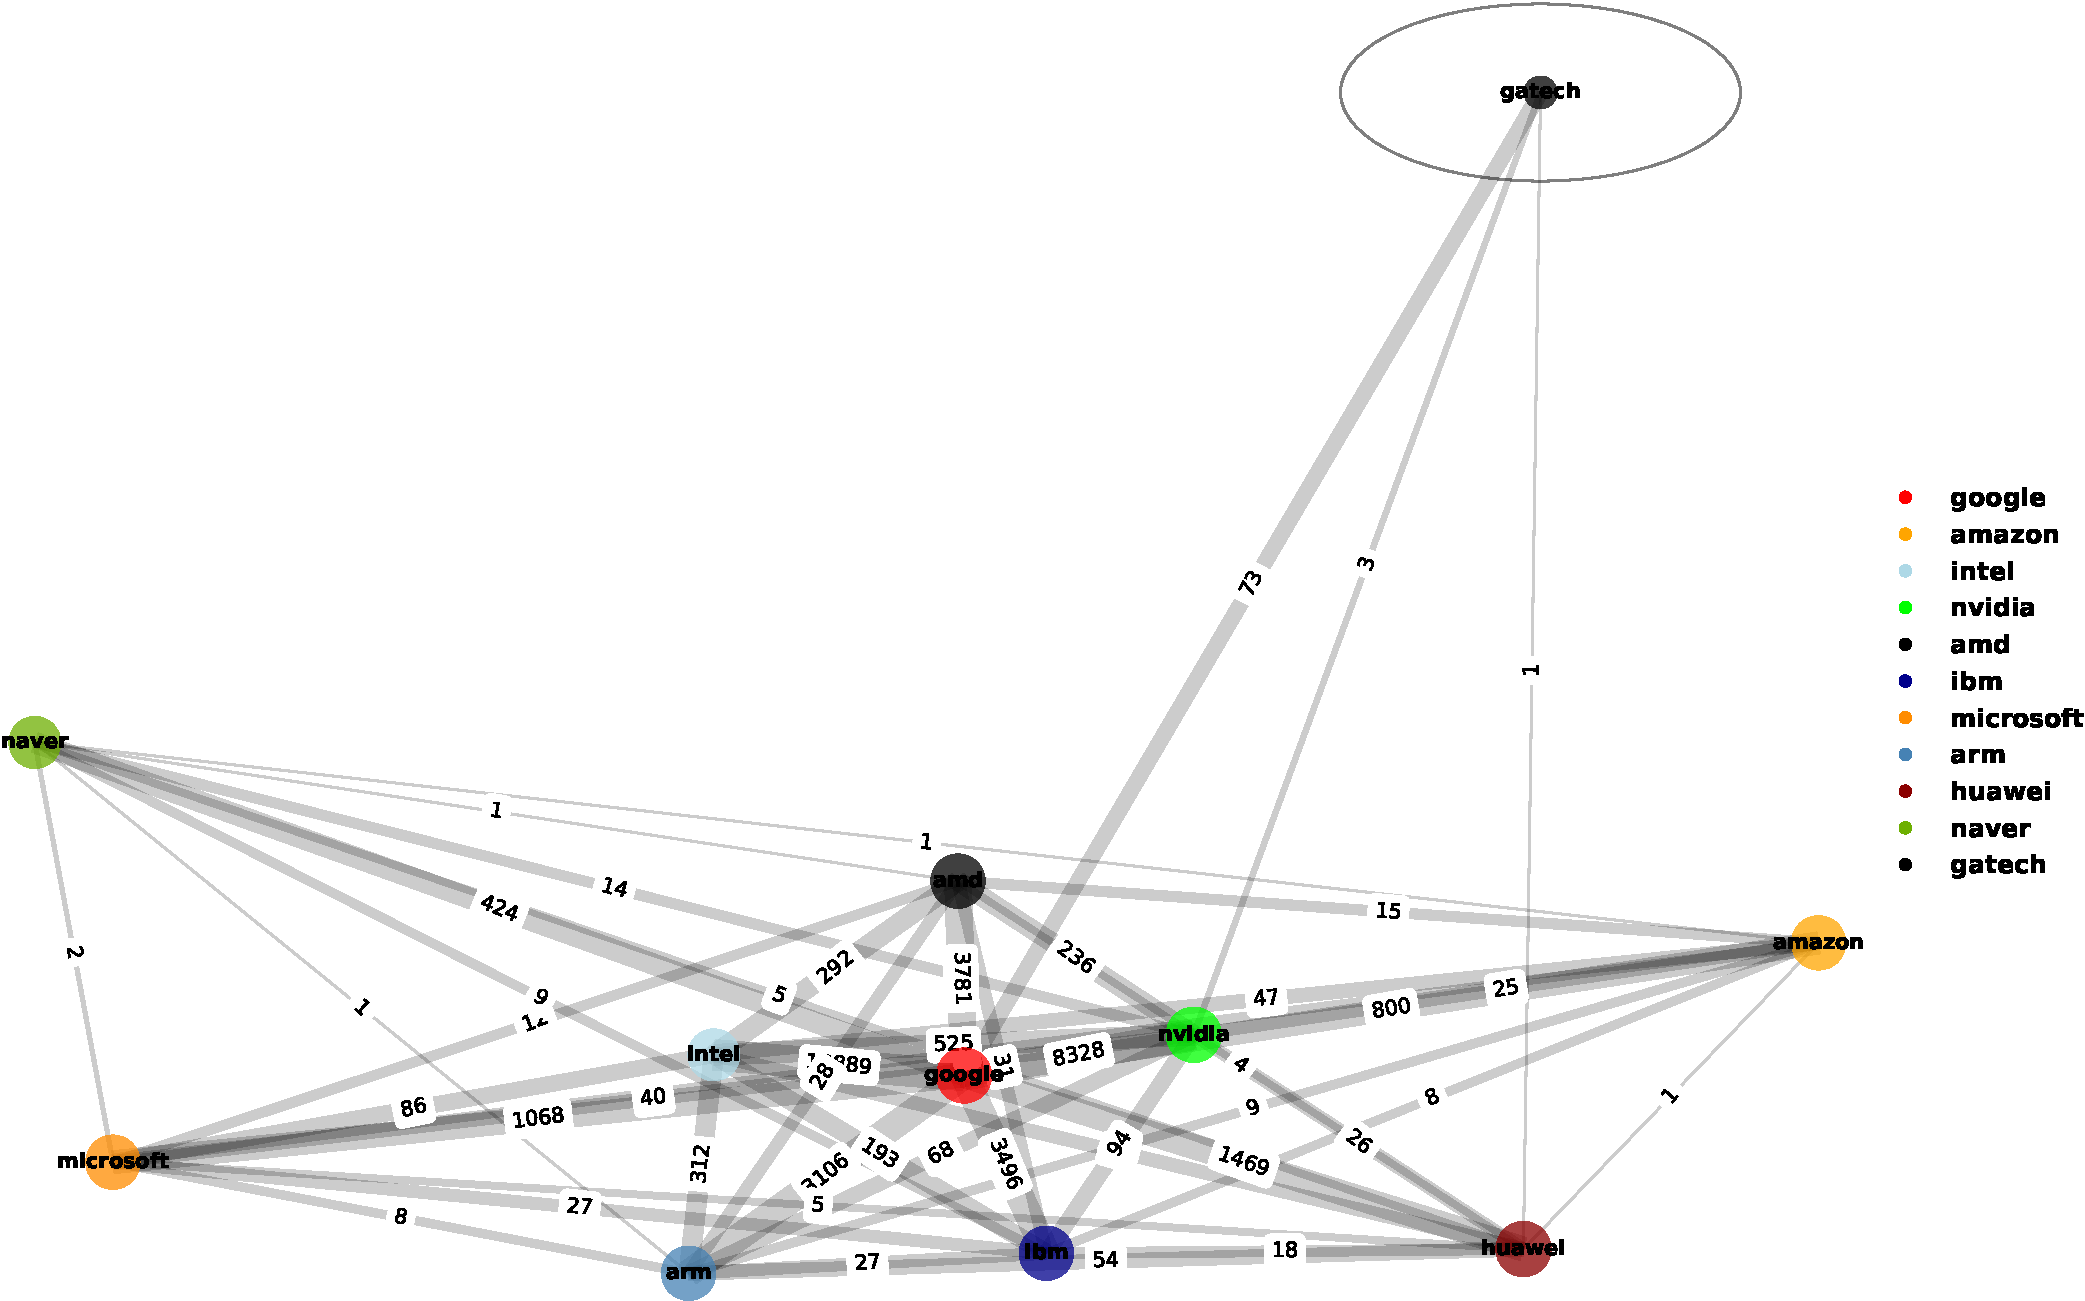
\includegraphics[keepaspectratio=true,width=0.9\textwidth]{./Figures/noo/gatech_cropped.pdf}
\caption{Scraplog output for gatech}
\label{figgatech}
\end{figure}
}


While conducting this research we learned that in the world of \ac{AI} deep learning, the infrastructure is not only about powerful computers with \ac{GPUs} or \ac{TPUs}. It is also about large amounts of memory and fast storage solutions, such as Solid-State Drives (SSDs) or distributed file systems, are crucial for managing vast datasets and model parameters that often deployed across multiple data center that require load balancing, parallelization efforts to work smoothly and consume fast amounts of electrical power and water for cooling. Many specialized frameworks, libraries and tools are also required for developing and optimizing deep learning models. Vast amounts of vast, clean, relevant, and readily accessible data are also important to deploy deep learning into production. The same applies to models, as the existence of reference pre-validated models is a key to developing newer and better models. 
So while some universities, research institutes and open-source communities might have access to powerful computing resources, Google can offer much more for deep learning that the hardware you can order from vendors it a very fast way to researchers interested in testing their latest models and algorithms for \ac{AI} or \ac{ML}.

As in prior covered universities and research institutes, by contributing to TensorFlow Georgia Tech can (1) advance research and education, (2) continue its strong tradition of supporting open-source initiatives, (3) bridge with the practice, industry and real-world applications, (4) nurture relationships with other leading institutions and industry players and, all while aligning with its strategy of leading in technology development and contributing to societal advancement through technological innovation.






\subsection{Pointing our lenses to MIT}


The seventh non-commercial organization that most contributes to the TensorFlow code is the  Massachusetts Institute of Technology which is commonly known as MIT.  The famous Technological University had six developers coding with the top ten commercial contributors to TensorFlow (see \Cref{tnoncomercial}) and the network shows five inter-organizational relationships. 
As visible \Cref{figgatech}, MIT similar to all other non-commercial players listed \Cref{tnoncomercial} has a strong tie with Google.  Besides the strong tie with Google, MIT had a less strong tie with Intel. It also had weak ties with AMD, Naver (bases in South-Korea) and Nvidia and IBM. Here we must point out that we only consider developers as affiliated with MIT if the email they used to commit code had the \textit{mit.edu} domain, we did not consider the \textit{alum.mit.edu}.  As the later email domain is provided by MIT Alumni Association we did not consider the association strong enough to associate developers with the MIT affiliation for this research purposes. We number of nodes in the collaborative inter-individual network affiliated with MIT would had three more nodes if considering the \textit{alum.mit.edu} domain. 



\iftoggle{TaFigOnEnd}{
\InsertHere{Figure}{Scraplog output for mit.}{\ref{fig:mit}}{10}
}
{
% Generated by 5-add-code-to-main.tex.sh 
\begin{figure}[h]
\centering
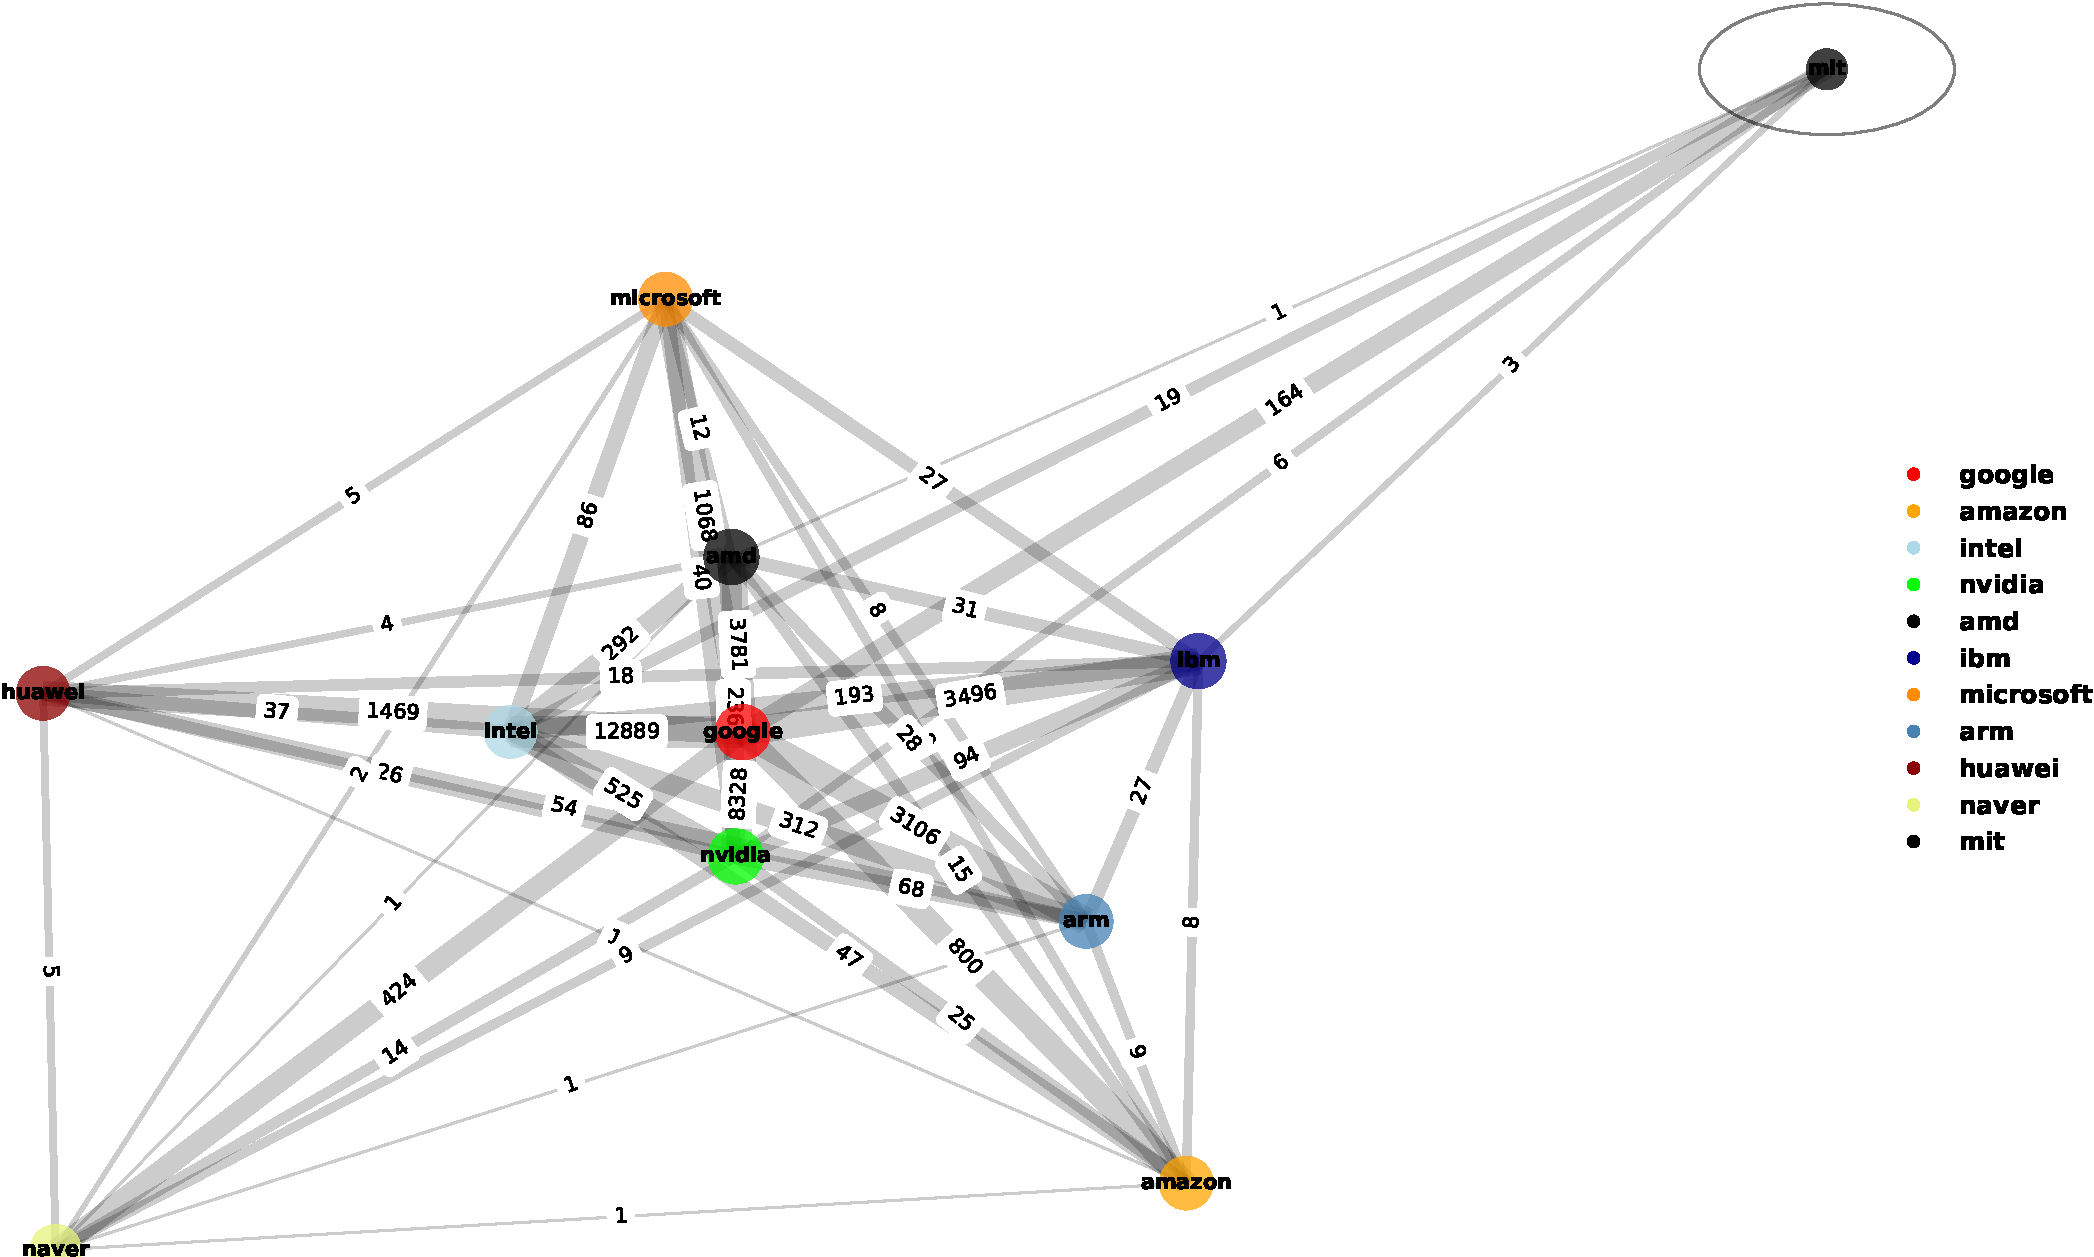
\includegraphics[keepaspectratio=true,width=0.9\textwidth]{./Figures/noo/mit_cropped.pdf}
\caption{Scraplog output for MIT}
\label{fig:mit}
\end{figure}
}


MIT have a strong association with the history of \ac{AI} for many decades. It brought to the table, expertise in Neural Network Optimization where the work by MIT researchers on optimizing neural networks has influenced TensorFlow's implementation.  Furthermore, MIT have been involved in the development of TensorFlow Federated, an extension of TensorFlow that facilitates federated learning. This library supports decentralized learning, where data remains on local devices and only model updates are shared, addressing privacy and data security concerns. 



From a educational perspective, MIT has used TensorFlow extensively in its educational materials, such as the MIT OpenCourseWare (OCW) courses on \ac{ML} and \ac{AI}. These courses provide practical training on TensorFlow, helping students and practitioners learn how to build and deploy machine learning models.  Many of the MIT courses expose students and future \ac{AI} practitioner to TensorFlow with hands-on experience on building neural networks in TensorFlow \footnote{See \href{https://ocw.mit.edu/courses/6-s191-introduction-to-deep-learning-january-iap-2020/}{https://ocw.mit.edu/courses/6-s191-introduction-to-deep-learning-january-iap-2020/} for example}.  The collaborative tie with IBM mirrors a formal partnership  between  MIT and IBM in the MIT-IBM Watson AI Lab, where TensorFlow is frequently used in joint research projects\footnote{See \href{https://mitibmwatsonailab.mit.edu/}{https://mitibmwatsonailab.mit.edu/}.}. 




% What the figure shows 

% Question 1 ,2, 3 an 4 







\subsection{Pointing our lenses to Apache}

% What the figure shows 

The eighth non-commercial organization with the most contributors to TensorFlow is not a university or a research institute. It was the Apache open-source community primarily maintained and orchestrated by the Apache Foundation. The Apache Software Foundation (ASF) was established in 1999 as a non-profit organization to support the Apache HTTP Server Project and its community of open-source developers. The origins of Apache trace back to 1995, when a group of developers, including Rob McCool and Brian Behlendorf, collaborated to enhance the NCSA HTTPD web server software, leading to the creation of the Apache HTTP Server. This server quickly gained prominence for its reliability, flexibility, and open-source nature. The success of the Apache HTTP Server catalyzed the formation of the ASF to manage and oversee the growth of a wide range of open-source projects beyond the original HTTP server. Today, the ASF hosts numerous high-impact projects such as Apache Hadoop, Apache Spark, and Apache Kafka, continuing to promote open-source software development through its collaborative and community-driven model. 

To our surprise, and as evidenced by \Cref{figApache}, the Apache organization is connected to all the top 10 organizational contributors to TensorFlow (see \Cref{tcomercial}) with 9 out of 9 possible inter-organizational edges. That connectedness beats even Chromium that was connected to 8 out of 9  possible inter-organizational edges (see \Cref{Chromium} to notice that Chromium is not connected with Naver). Here, we must point out that open-source communities like Chromium and Apache establish more edges with the top 10 organisational contributors than universities and research institutes. This highlights their important role in the TensorFlow community as both TensorFlow, Apache and Chromium want to ensure compatibility and interoperability of their code-base. 


Apache projects, such as Apache Hadoop and Apache Spark, provide frameworks for distributed data processing and storage, which are essential for handling the large-scale datasets typically used in machine learning tasks. TensorFlow, on the other hand, is a powerful machine-learning framework designed for building and deploying machine-learning models. They are therefore very complementary platforms.  The integration of TensorFlow with Apache projects allows for better data processing pipelines. 
For example, TensorFlowOnSpark is an open-source framework that combines TensorFlow's machine learning capabilities with Apache Spark's efficient data processing and distributed computing power. This integration enables the training of machine learning models on large datasets stored in Hadoop's HDFS or processed using Spark, thus facilitating scalable and efficient machine learning workflows. Developers typically rely on formats, tools and libraries provided by the Apache foundation for processing data before loading them into machine learning workflows.  Furthermore, Apache Beam, another project under the Apache Software Foundation, offers a unified programming model to define and execute data processing pipelines, which can be integrated with TensorFlow Extended (TFX) for building production-scale machine learning pipelines. This collaboration enhances the ability to preprocess data, train models, and deploy them in a scalable and efficient manner, leveraging Apache's strengths in big data processing and TensorFlow's advanced machine learning algorithms. 

On the one side, it is in the interest of the Apache Foundation to ensure that their solutions (e.g., Apache Hadoop and Apache Spark)  integrate very well with TensorFlow. If Apache projects seamlessly integrate with TensorFlow they become more attractive and useful, they grow with each other.  On the other hand, improving the interoperability between TensorFlow and Apache projects can result in more efficient data processing and model training workflows, which benefits both platforms and their users.  When starting and evolving TensorFlow, Google and its partner did not need to reinvent the wheel. They could for example benefit from a from a number of ready-available open-source projects such as: (1) the Hadoop's Hadoop Distributed File System (HDFS) offers a highly scalable and fault-tolerant storage solution that can handle vast amounts of data across many distributed nodes making it ideal for storing the large datasets required for training deep learning models in TensorFlow, (2) the  Hadoop's MapReduce and YARN (Yet Another Resource Negotiator) frameworks enable distributed data processing across a cluster of computers, (3) the Apache Spark analytics engine that offers in-memory data processing capabilities that can speed up data preprocessing and transformation tasks before feeding data into TensorFlow models, (4) the Apache Beam provides a unified programming model for batch and stream data processing, which can be integrated with TensorFlow  to build end-to-end machine learning pipelines that handle data ingestion, preprocessing, model training, and serving, and (5) the Apache Kafka is used for real-time data streaming and ingestion. It would cost immense time and money for Google to re-write this well-established community-driven projects orchestrated by the Apache Foundation. 


\iftoggle{TaFigOnEnd}{
\InsertHere{Figure}{Scraplog output for apache.}{\ref{figApache}}{10}
}
{
% Generated by 5-add-code-to-main.tex.sh 
\begin{figure}[h]
\centering
\includegraphics[keepaspectratio=true,width=0.9\textwidth]{./Figures/noo/Apache_cropped.pdf}
\caption{Scraplog output for Apache}
\label{figApache}
\end{figure}
}
 
As evidenced by the following quote that also emerged during a second semi-structured interview with a TensorFlow developer recruited via e-mail and LinkedIn, TensorFlow depends on multiple open-source software projects. 

\begin{quotation}
``We would not exist without many other open-source projects'' ... ``for example Python, NumPy, the Linux Kernel and the GNU tools for processing text." Also Bazel, nGraph ' ... `` we also integrated Keras' that started as an independent open-source project'.   -- Software developer  and regular contributors to the TensorFlow during a semi-structured interview with the first author.  Pseudonym Berta. 
\end{quotation}


Similarly to the Chromium project, but at a larger scale, the Apache Foundation also play a very important dual role (1) maintaining the software code base of multiple open-source projects that for several reasons can not be turned into commercial software, and (2) be a neutral place that ensures openness and transparency in the orchestration of collective goals of the different project contributors. In the case of Apache, we learned that ``Required behaviours', ``Voting'' and ``Consensus'' play a very important role in deciding the direction of the Apache projects under the foundation umbrella. 



% Question 1 ,2, 3 an 4 

% Generated by 5-add-code-to-main.tex.sh 


\subsection{Pointing our lenses to KTH}

% What the figure shows 

The ninth non-commercial organization is the Royal Institute of Technology (Swedish: \textit{Kungliga Tekniska Högskolan} commonly known as KTH. Based in Stockholm, Sweden, founded in 1827, is one of Europe's leading technical and engineering universities.  KTH hosts several institutes and labs dedicated to \ac{AI} and \ac{ML}. Among them is the KTH AI Research Centre, which focuses on advancing AI technologies and their applications across various domains. Additionally, KTH collaborates with the Swedish AI Society (SAIS) and participates in multiple AI and machine learning projects, both nationally and internationally having success in securing both EU  and National R\&D funds for AI research.  
The university's School of Electrical Engineering and Computer Science is particularly active in AI research, with specialized labs such as the Robotics, Perception, and Learning Lab (RPL) and the Division of Speech, Music, and Hearing. 

As visible in the computer-generated \Cref{figkth} obtained by mining the TensorFlow repository with Social Network Analysis, KTH has a strong tie with Google and several weaker ties with Naver, Nvidia, IBM (who have offices nearby KTH), AMD and Intel.  Some \ac{AI} and \ac{ML} startups born at KTH. One example is Logical Clocks, a Swedish startup founded in 2016 by a team of researchers from KTH, which is one of the notable success stories emerging from KTH’s academic environment. The company was established by experts in distributed systems and big data, who were involved in significant research projects at KTH. Logical Clocks is best known for developing Hopsworks, a data platform that features the world’s first ``Feature Store'' for machine learning, which integrates seamlessly with TensorFlow. The collaboration between Logical Clocks, Google and KTH, which is to a large extent publicly funded, enhances TensorFlow's functionality, particularly in handling big data and distributed machine learning tasks therefore bringing value from public money spent on research and education in the past back to to the society as a whole. 


\iftoggle{TaFigOnEnd}{
\InsertHere{Figure}{Scraplog output for kth.}{\ref{figkth}}{10}
}
{
\begin{figure}[h]
\centering
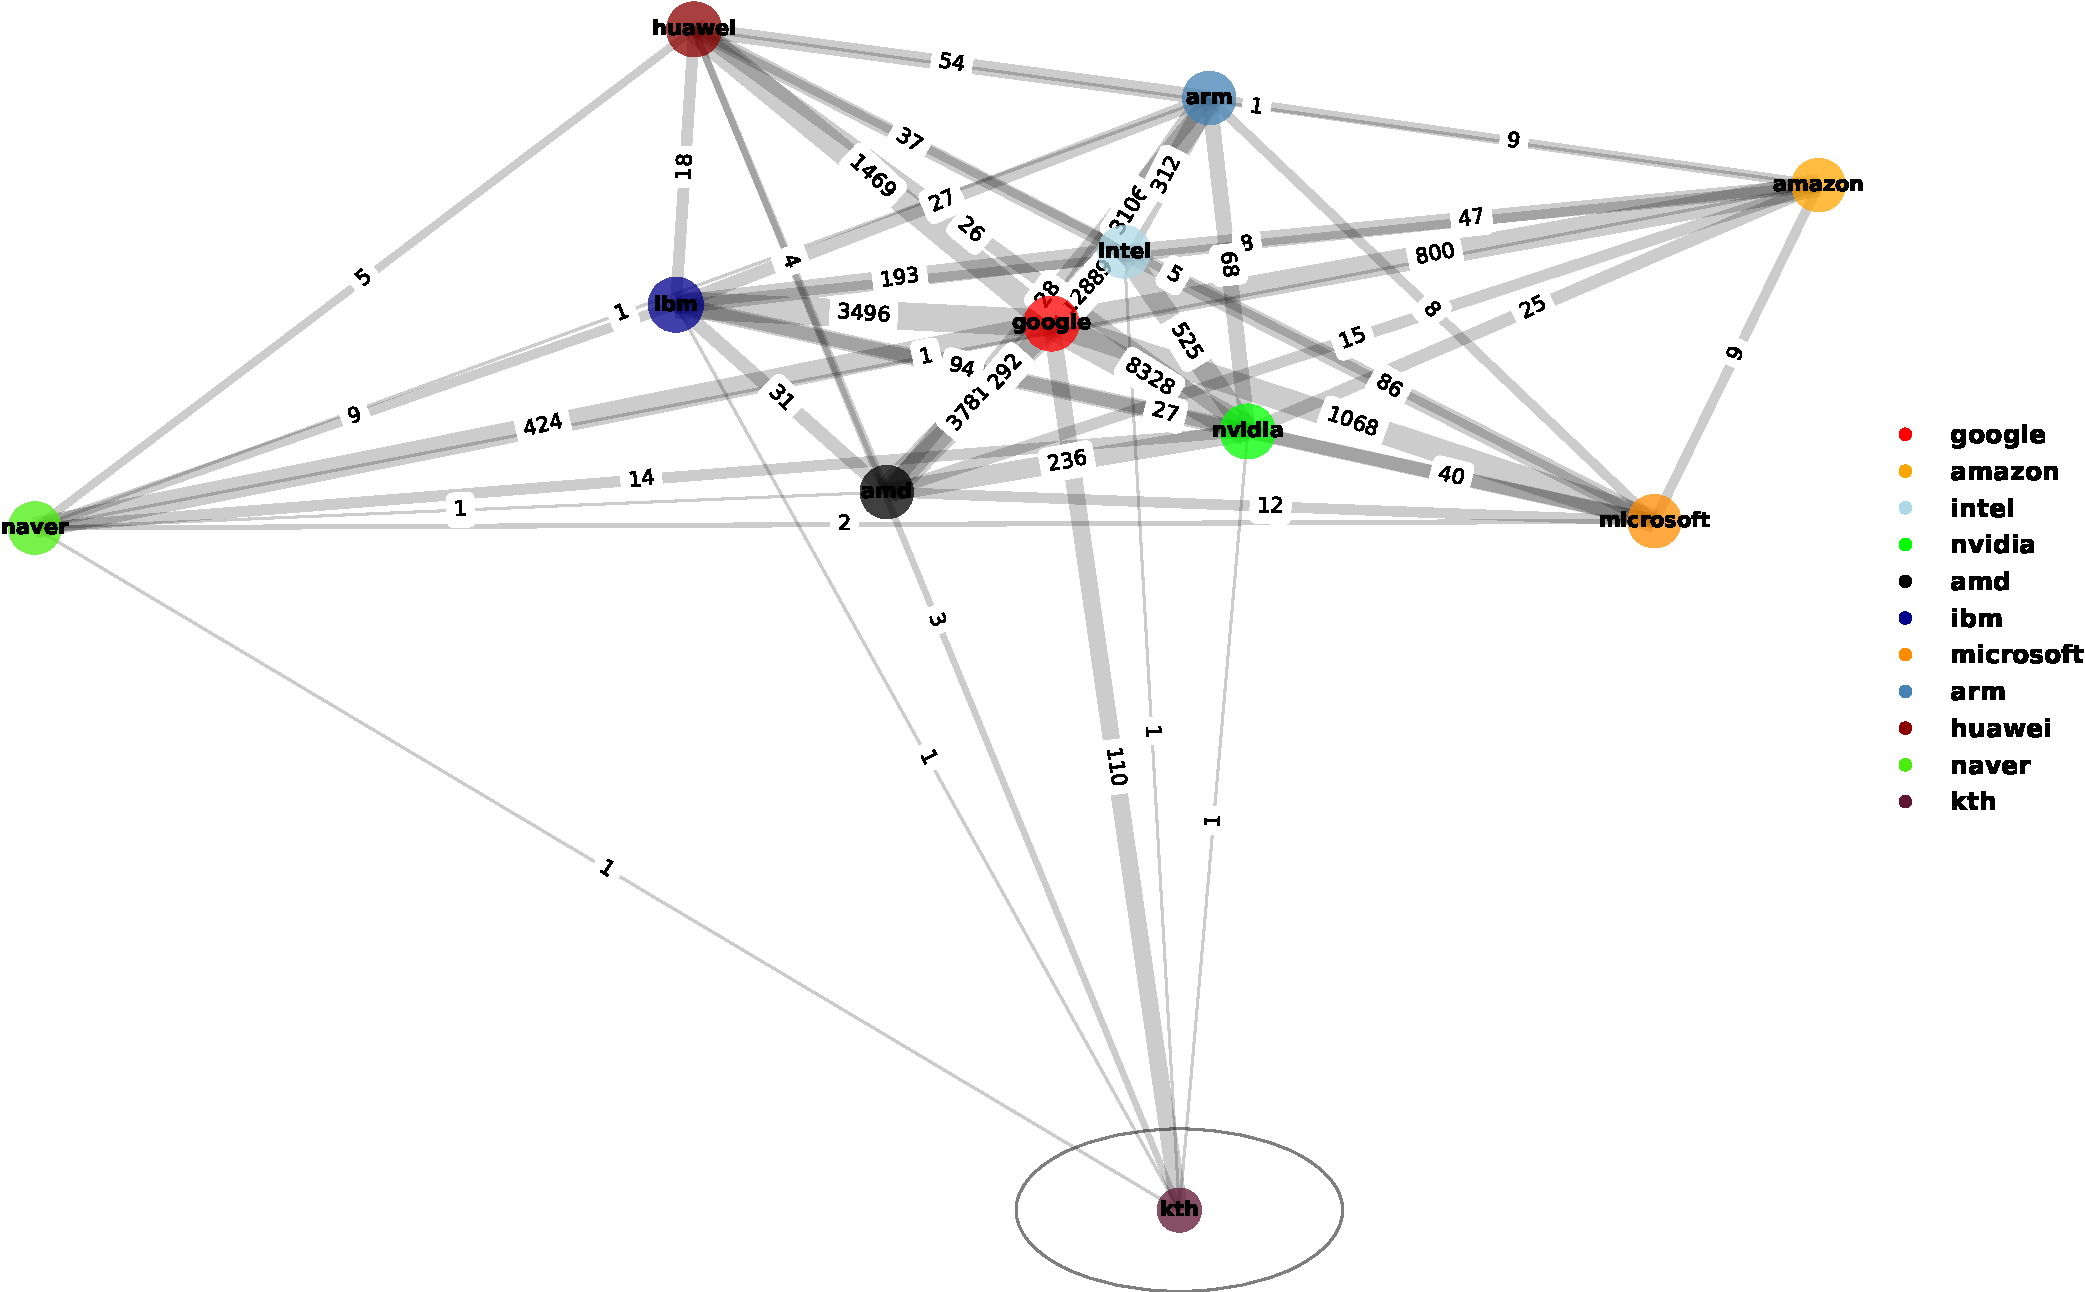
\includegraphics[keepaspectratio=true,width=0.9\textwidth]{./Figures/noo/kth_cropped.pdf}
\caption{Scraplog output for KTH}
\label{figkth}
\end{figure}
}


Contributions from KTH  to the TensorFlow ecosystem have included enhancements to its distributed training capabilities, improvements to data ingestion and pre-processing pipelines, and the development of new tools and libraries that extend TensorFlow's functionality. Those are important as the training of complex models does not fit in one big machine. The work needs to be distributed across machines and process the aggregated results back - a very complex task as the allocation of computing resources is often limited, failures might occur across heterogeneous computing nodes and bottlenecks need to be minimized. 
From KTH side, the motivations to contribute go along the same lines as the Universities we covered before. Continue leading \ac{ML} research as one of the \ac{ML} research pioneers, showcasing unique technical competencies in \ac{AI} and \ac{ML}, curating industry-academia partnerships that are important for obtaining research grants in the EU and Swedish systems.  Furthermore, researchers developing the latest \ac{AI} and \ac{ML} concepts, algorithms, models and tools can see their work applied in the real world via the TensorFlow ecosystem and the computing Infrastructure provided by Google and its partners.  






% Question 1 ,2, 3 an 4 

% Generated by 5-add-code-to-main.tex.sh 

% Generated by 5-add-code-to-main.tex.sh 


% Pretending I forgot 
\subsection{And finally, pointing our lenses to Berkeley}

% Grammally checked 5 Aug 2024
The tenth non-commercial organization that most contributes to the TensorFlow code is The University of California, Berkeley also commonly known as UC Berkeley or simply Berkeley.  The university is associated with many technological advancements that are in the public domain such as (1) the RISC-V chipset design instruction set released under a royalty-free open-source license released by Berkeley in the 2010s, (2) the Berkeley Software Unix Distribution (aka BSD) that played a very important role in powering servers, workstations and networking equipment during the 1980s, (3) the SPICE simulator that became the worldwide standard integrated circuit simulator, or (4) the TCL/TK programming language languages that remain very a popular choice for applications that need portability and graphical user interfaces that work across different operating systems.  The Berkeley campus regularly hosts several open-source conferences for academics and practitioners (e.g., the Open Source Summit North America and the Scylla Summit) mounting evidence that Berkeley is not disconnected from the open-source world. 


% Grammally checked 5 Aug 2024
As visible in the computer-generated \Cref{figberkeley}, Berkeley has a strong tie with Google and several weaker ties with Naver, AMD, Intel, Nvidia, IBM, and ARM. Here, it is important to note that even though Berkeley is geographically closer to Google, its position on the TensorFlow in the TensorFlow collaborative network is similar to other universities located somewhere else like MIT, SNU and the DFKU. The collaborative network in \Cref{figberkeley} also evidences that Berkeley is connected collaboratively to the big chipset makers (i.e., AMD, Intel, Nvidia, and ARM), something that is also visible in the RISC-V and SPICE open-source ecosystems.  Contrary to many other non-commercial organisations covered by this study, Berkeley does not collaborate with the biggest vendors of cloud computing services (i.e., Microsoft and Amazon). 



% BOTS-ADD-HERE

% What the figure shows 

% Question 1 ,2, 3 an 4 

% Generated by 5-add-code-to-main.tex.sh 




% Generated by 5-add-code-to-main.tex.sh 

\iftoggle{TaFigOnEnd}{
\InsertHere{Figure}{Scraplog output for berkeley.}{\ref{figberkeley}}{10}
}
{
\begin{figure}[h]
\centering
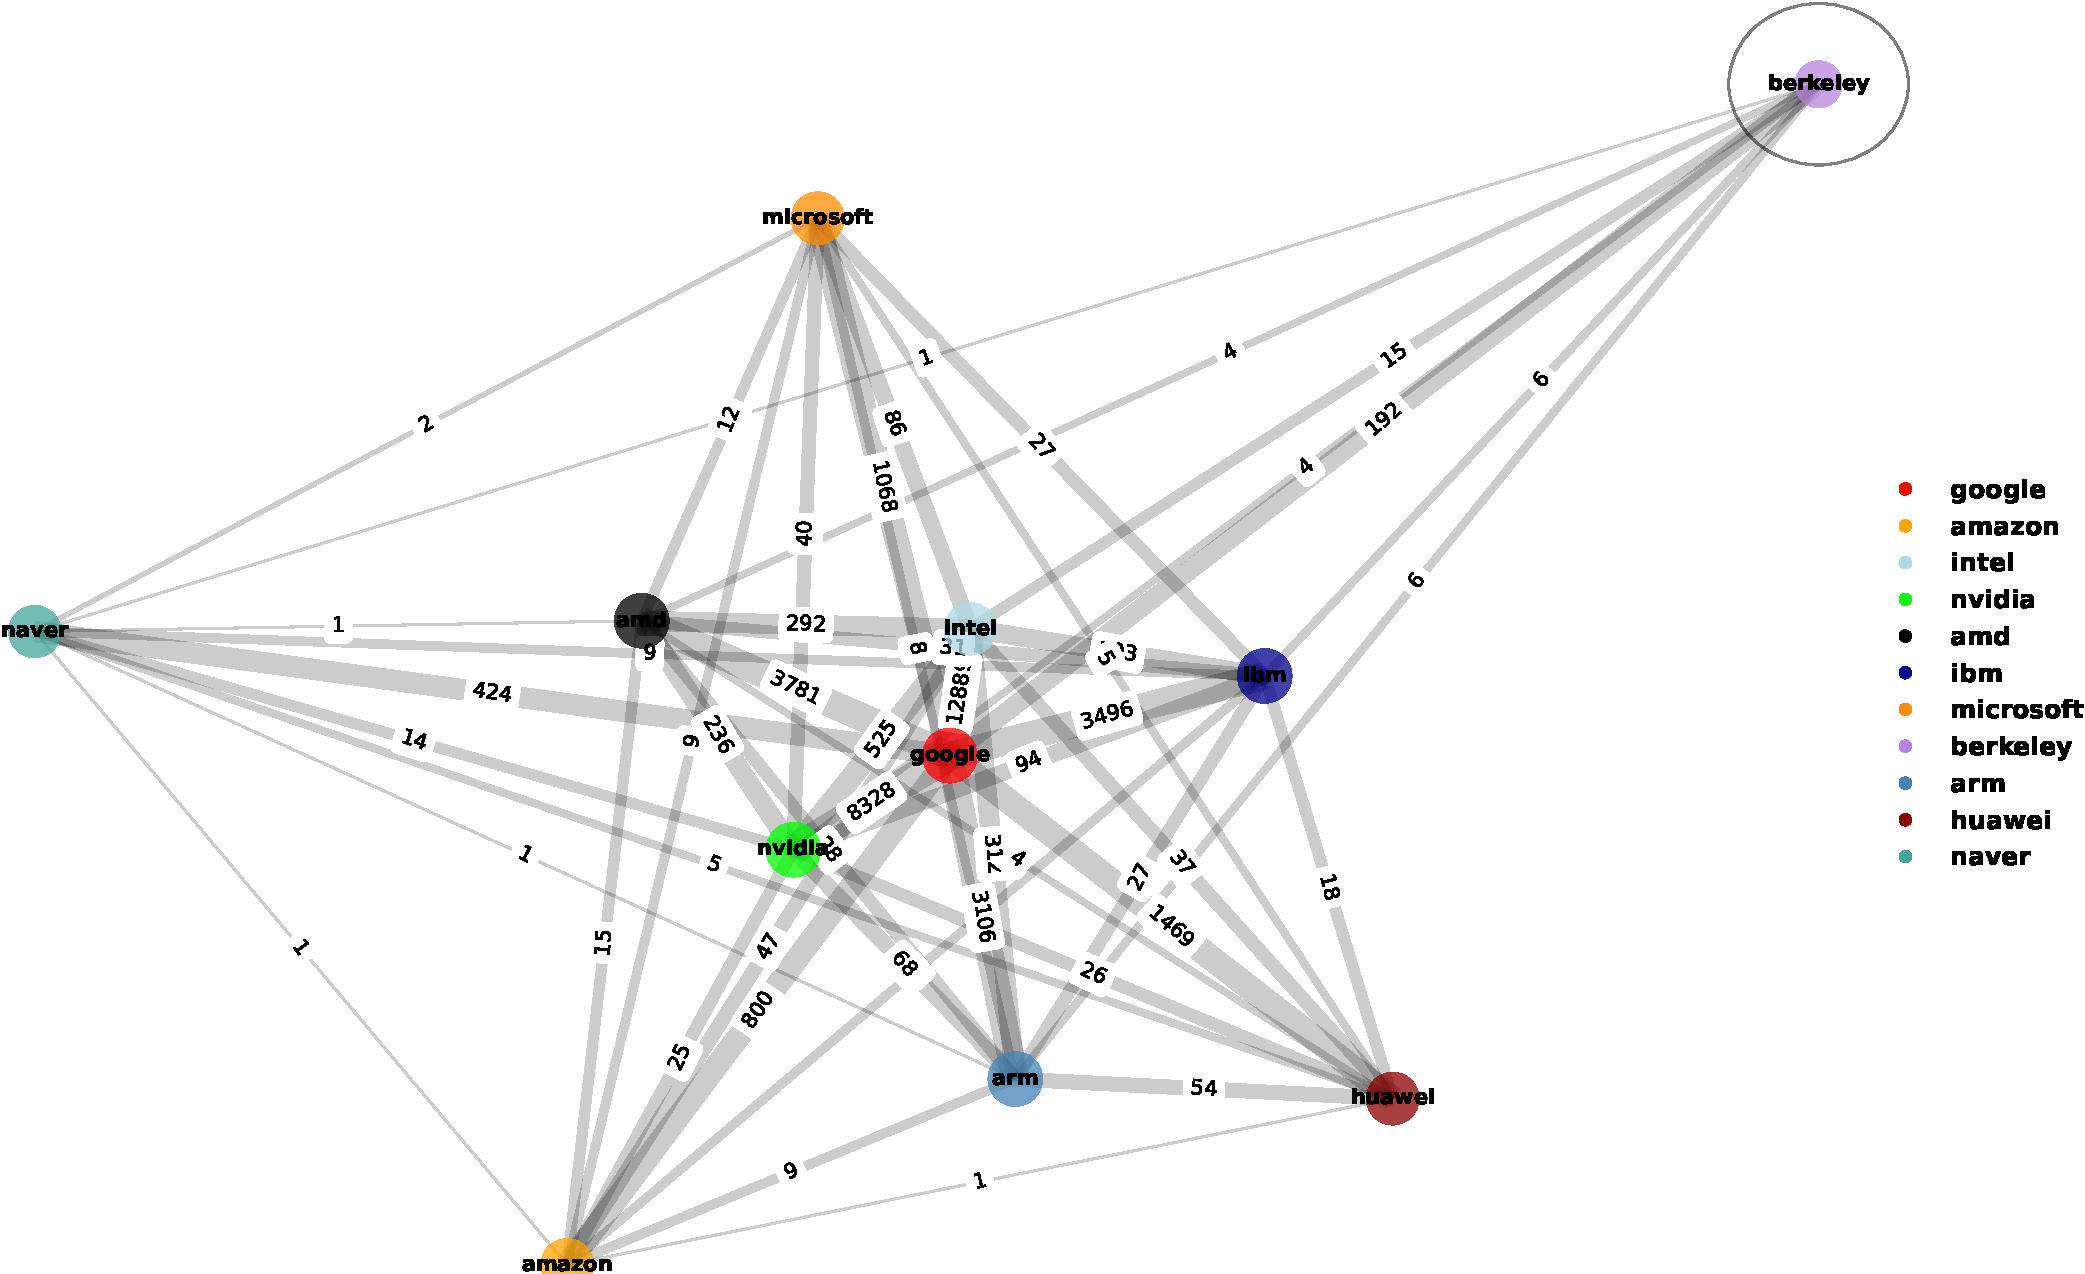
\includegraphics[keepaspectratio=true,width=0.9\textwidth]{./Figures/noo/berkeley_cropped.pdf}
\caption{Scraplog output for berkeley}
\label{figberkeley}
\end{figure}
}

Berkeley University hosts two labs that play an important role in the TensorFLow ecosystem. The Berkeley Artificial Intelligence Research (BAIR),  contributed to TensorFlow by developing new algorithms and techniques for \ac{ai} and \ac{ml}. Another lab hosted by Berkeley, the Algorithms, Machines, and People Lab (AMPLab), with expertise in large-scale data processing and distributed computing, has helped improve TensorFlow's capabilities in these areas. Berkeley's expertise in the realm of chipset design and operating systems contributed to Google's and Intel's efforts to improve TensorFlow's performance on Intel processors and accelerators. Even if Nvidia currently designs the most desired chips for \ac{ai} and \ac{ml} applications, due to the number of cores available for matrix multiplication within a single chip \citep[see][]{Reuther_et_al2019}, the processors of Intel are still the most deployed one across servers and clouds worldwide. Therefore, it from the interest of both Intel and Google to improve TensorFlow's performance on Intel processors and accelerators. Otherwise, consumers might move to other platforms.  Berkeley expertise offered not only expert consulting, but also code contributions from faculty scholars and students who co-developed new features, bug fixes, and performance improvements, which were shared with the broader TensorFlow community.


By engaging in the co-production efforts of TensorFlow, Berkeley advanced research and innovation, enhanced the educational resources, boosted their students and staff with competencies that are appliable in the real-world, cultivated relations with strong industrial leaders, and showcased their abilities to improve the performance and scalability of \ac{ai} and {ml} training environments by tuning the software layers of code that work closer to the hardware and interface with the operating systems, CPUs and GPUs.   Furthermore, UC Berkeley continued its strong tradition of supporting open-source projects, which aligns with the collaborative and accessible nature of academic research.  In our view, this makes sense as much of the excellence comes from projects that are publicly funded by state and federal budgets. 



\subsection{The \textit{Why} of co-producing TensorFlow in an open and coopetitive way}



After reporting our results centred around the top ten non-commercial organizational contributors to TensorFlow and how they work with the top commercial contributors to TensorFlow, it is now time to report on why co-producing TensorFlow in an open and coopetitive way.  Or in some other words,  \textbf{Why not co-producing in the traditional proprietary way that emphasises centralized control and intellectual property rights ?}. First, we take the perspective of the Google high-tech giant that started TensorFlow as an open-source project, and then the perspective of its non-commercial partners in the TensorFlow platform ecosystem. 



From the perspective of Google, we could identify four reasons to open up TensorFlow from the collected evidence. First, 
by doing it in an open-source way, Google could integrate and build on top of established open-source technologies such as the ones provided by the Python, NumPy, GNU, Linux, Apache and Chromium communities. It would be expensive and time-consuming for Google to ignore those open and ready-available technologies under a permissive intellectual property regime\footnote{Note here that while the distribution license terms of those technologies allow Google to integrate them, they force Google to keep TensorFlow open as well, including to its competitors.}. A second reason is scientific prestige, as noted in the following quote by a Google employee, Google researchers had mixed feelings about external entities developing tools or technologies directly derived from Google's own research efforts. On the other way, Google was criticized in the scientific community for publishing new ideas, new models, and new results, but not sharing the blueprints (e.g., the model definition, or the software implementation). By providing the source code of the software related to new \ac{AI} or \ac{ML} advances presented at prestigious conferences, Google boosted its reputation and gained trust from leading researchers \ac{AI}, \ac{ML}, computer vision and sound recognition from academia and industry experts. They stopped doing tools using Google's latest research, instead, they started implementing their ideas, models and tools on top of TensorFlow. Both sides benefited from the flow of expertise, ideas, models, and tools in the the platform ecosystem. 

\begin{quotation}
``After we published a paper, we could see that new open-source tools would come up in just a few weeks based on our latest research. Then we publish another paper, another model, or another algorithm. And guess what, somebody would come with a new tool or a new module just doing that.'' -- Machine Learning researcher with expertise in computer vision, Google employee and regular contributor to TensorFlow during a semi-structured interview with the first author.  Pseudonym Charles.
\end{quotation}

Third, and another valid motivation for doing it in an open-source way are the practical benefits of producing software in the public domain. The open-source approach fosters a collaborative environment where diverse developers, researchers, and organizations can contribute to TensorFlow's evolution. No individual or organization needs formal or approval to contribute to work on their innovation.  All without much time negotiating IP licensing agreements, software end-user agreements,  implementing gate-keeping and access-control procedures and mechanisms, and knowledge-sharing tensions that characterise the software business as usual often in supplier-client relationships. And all in the public domain over the Internet, where being far from Google does not seem to be a big problem to contribute to TensorFlow. 
Furthermore, by making TensorFlow freely available with models and curated data with it, Google established it as a standard machine learning platform. Widespread adoption by academic, research, and industry organizations promotes its use and strengthens Google's position in the AI ecosystem and the AI hype of the 2010s. Also importantly,  it removed and reduced barriers for others to play with \ac{AI} and \ac{ML} increasing the overall size of the market and creating demand for complementary products and services such as applications with \ac{AI} features, 
rentable cloud computing power and TPUs that are specially designed to optimize the deep matrix multiplication operations for training \ac{AI} and \ac{ML} models. 


From the point of view of non-commercial organizations, out research results data aggregated and evidenced ten motivations for contributing to the TensorFlow. To our surprise, the analysis centered around ten non-commercial organization unveiled to ten motivation to contribute to a open-source and coopetitive platform ecosystem such as TensorFlow as we following enumerate: 

\begin{description}
\item[Advancing research and innovation] Non-commercial entities, such as universities and research institutes, engage in TensorFlow's development to stay at the forefront of AI and machine learning research. Participation allows these entities to pursue cutting-edge projects, pushing the boundaries of existing knowledge and technology in AI and ML.

\item[Showcasing specialized competence] Contributing to a high-profile open-source project like TensorFlow provides an opportunity for non-commercial entities to demonstrate their technical expertise and specialized competencies in AI and ML. This can enhance their reputation and attract further research funding and collaborations. This is also important for open-source communities and their respective foundation so that they can also showcase their technical solutions and competences. 

\item[Accessing world-class infrastructure] Collaborating on TensorFlow provides non-commercial entities access to Google's extensive computational resources and infrastructure, which might otherwise be unattainable. This access enables them to conduct large-scale experiments and research that require significant computational power.

\item[Facilitating partnerships] By contributing to TensorFlow, non-commercial entities can ``expose'' themselves form partnerships with industry leaders, such as Google, and other academic and industrial institutions. These partnerships can lead to collaborative research projects, increased funding opportunities, and shared expertise that can be immediate or in the long run. 

\item[Setting up communities of knowledge] Engaging with TensorFlow allows non-commercial entities to participate in and help build a global community of AI and ML researchers and developers. This community fosters the exchange of ideas, best practices, and innovations, accelerating the overall progress in the field.

\item[Enhancing educational programs] Contributions to TensorFlow can have significant educational benefits. Non-commercial entities can develop educational resources, such as tutorials and courses, based on their hands-on experience with TensorFlow, which helps train the next generation of AI and ML researchers and practitioners.

\item[Societal impact] Non-commercial entities are often motivated by the potential societal impact of their contributions. By advancing AI and ML technologies, they can address real-world problems and contribute to societal well-being, such as through advancements in healthcare, environmental monitoring, and more. To our view, there is natural desire of seeing their theoretical advancements in practice in the real world. 

\item[Institutional recognition] Participation in TensorFlow enhances the global reputation of non-commercial entities, positioning them as leaders in AI and ML research. This recognition can attract top talent, students, and additional funding to the institution.

\item[Influencing the development agenda] By contributing to TensorFlow, non-commercial entities can influence the direction and priorities of AI and ML development. This ensures that their research, business, social or technological interests and goals are considered in the evolution of the platform. This is especially important for organization that want TensorFlow to evolve according their own interests. 

\item[Ensuring interoperability] Contributions from diverse organizations help ensure that TensorFlow remains interoperable with various systems and technologies. This  compatibility encourages widespread adoption and integration of TensorFlow with different tools, libraries, solutions and services. This is especially important for open-source projects and respective foundations that want TensorFlow to integrate well with their code-base. 
\end{description}


We finalize our results section with \Cref{tmotivations} that maps motivation to each non-commercial organization  before discussing how our results integrate with extant theory.

\begin{table}[h]
 
\caption{Motivations for non-commercial entities to contribute to the TensorFlow open-source platform for AI and ML. \label{tmotivations}}

\begin{tabularx}{\textwidth}[]{lcccccccccc}
\toprule
& SNU & DFKI & Chromium & ISP & PKU & GTech & MIT & Apache & KTH & Berkeley\\
%Motivations &  &  &  &  &  &  &  &  & \\
\midrule
Advancing research \& innovation & × &  × &  & × & × & × & × &  & × & × \\
Showcase specialized competence & × & × & × & × & × & × & × & × & ×  & ×\\
Accessing unique infrastructure & × & × &  & × & × &  &  & × &  × &  \\
Facilitating partnerships & × & × &  & × & × &  &  & × & ×  & × \\
Setting up knowledge communities & × & × &  & × & × & ×  & × & × & × & × \\
Enhancing educational programs & × &  × &  & × & × & × & × &  & × & × \\
Societal impact & × &  × &  & × & × & × & × &  & × & × \\
Institutional recognition & × & × & × & × & × & × & × & × & ×  & ×\\
Influencing development agenda & × & × & × &×  & × & × & × & × & ×  & ×\\
Ensuring interoperability &  &  & × & × &  &  & × & × &  × & × \\
\bottomrule
\end{tabularx}
\end{table}


\section{Discussion}



% Grammaly checked 28 of april  
Our research addressed a direct call by \citet{CzakonSrivastava_et_al2020} that stated the importance of knowing ``why and for which outcomes companies use more and more open source in communities including their competitors''~\citep[][]{CzakonSrivastava_et_al2020}.  By addressing the research questions \textit{``Why do tech giants like Google open-source advanced and complex technological platforms that started in-house?''},  \textit{``Why are different organizations cooperating with their competitors in the co-production of those open-source platforms?''} and and \textit{``Why non-commercial organizations contribute to the co-production of those open-source platforms?''}, we aim to increase our understanding of the open-coopetition phenomena. As a consequence of our theoretical interests, we also end up narrating the first circa ten years of TensorFlow with complementary visualizations of its social structure. Furthermore, to be able to explain the 'computerized' social network visualizations over time we also came across plenty of naturally occurring qualitative material that explained why Google open-sourced TensorFlow. Furthermore, we also came across material explaining the emergence of "communities of competitors"  in the co-production of TensorFlow.  All within the triple-helix framework. 

% Key results 


% Grammaly checked 28 of april 
The first surprising empirical results are captured in \Cref{figall}. Many of the code contributions to TensorFlow were identified with email accounts commonly associated with personal use (i.e., gmail, hotmail, yahoo, outlook and Chinese equivalent QQMail). We noted that many researchers associated with universities, research institutions and startup founders contributed using personal email accounts. In this sense, Google was successful at opening innovation processes via the open-source community. Like in other cases of open-coopetition in the automotive industry \citep[see][]{teixeira2023icis}, they open up to get third-party contributions from enthusiasts, students, hackers and academics among others. In the words of Teixeira, ``no one should need a permit to innovate on top of their product platforms'' \citep[p.~6][]{teixeira2023icis}. In this case, we noted that Google got many contributions from researchers in Germany, Russia, Cyprus, Portugal, France, Japan, Korea, South Africa, Australia, and many other geographies miles away from the Google office where TensorFlow was first developed. Innovation was not confined to a regional cluster. 

% crowdsourced innovation 
% See https://hub.packtpub.com/Google-opensorced-TensorFlow/

% Grammaly checked 28 of april 
The second surprising empirical result is visible in many of the figures capturing collaboration among the top 10 contributors without counting Google.
We can note that chipset makers (i.e., amd, Nvidia, arm, and intel), and cloud computing vendors (microsoft, amazon, and ibm ) have developers collaborating directly with
each other. This is in the sense that they co-edit the same source-code files of the TensorFlow code repository. They are not only in coopetition solely with Google in
the ecosystem, they are also in coopetition with many other direct competitors while fighting for the same revenue in globalized markets.  In this sense, these results
align with prior studies that found low levels of homophily by company affiliation in the production of complex software ecosystems
\citep[see][]{teixeira_et_al2020_homophily_linux_kernel,NguyenDucCruzes_et_al2019}. 

%It seems that developers identify with the community and feel
%comfortable co-producing software with their competitors.





% Third tis the job opening -- Leave du to lack of space 

%% Really work with each other 
%%% Intereviews, discussion, dicusssion dorums, etc 

% Preliminary answers to the guiding research questions:

%% Inteeviwew 
 
 Even if our research questions were theoretically driven, in order to explain the evolution of 
 %the social structure of 
 TensorFlow %captured 
 year after year, we came across naturally occurring qualitative material that directly addressed \textit{Why do tech giants like Google open-source advanced and complex technological platforms that started in-house?}. That qualitative material often taking the form of
 interviews\footnote{See for example the interview with Rajat Monga  that leads the R\&D of TensorFlow at Google, conducted by Lex Fridman, a YouTuber and research scientist at the MIT Laboratory for Information and Decision Systems. Transcript publicly available at \href{https://transcript.lol/read/youtube/@lexfridman/652310c5033150beacd17e4e}{https://transcript.lol/read/youtube/@lexfridman/652310c5033150beacd17e4e}.}, televised expert commentaries\footnote{See \textit{Why Google wants everyone to have access to TensorFlow} via Fox News \href{https://www.foxnews.com/video/4611174773001}{https://www.foxnews.com/video/4611174773001}.}, and Internet forums\footnote{See \href{https://www.quora.com/Why-did-Google-open-source-TensorFlow-Whats-in-it-for-them}{https://www.quora.com/Why-did-Google-open-source-TensorFlow-Whats-in-it-for-them}.}, was rich and explanatory even if not provoked by us. While many wonder why giving up so much intellectual property already on the table, many outlined other explanations such as crowd sourcing innovation, fomenting open-innovation, resource complementary, sharing risk, increased cooperation with researchers, enhancing collaborative efficiency in product development, practical benefits that can lead to faster product development and maintenance, reuse of software artefacts, exposition of the technology to thousands of developers in the open-source community as well as fearing the threat of new entrants to the market.


% Grammalu checked 8 of April 
While the set explanations from the previously mentioned qualitative material were already covered by literature in open-source, open-innovation, user-innovation, coopetition, and open-coopetition \citep[see~e.g.,][]{von2005democratizing,RoyChesbrough_et_al2018,BengtssonKock2014,teixeira2023icis}, we did find another novel explanation (i.e., expected outcome) for releasing software in an open-source way - that is \textbf{increasing the market size for the technology}. As Google released TensorFlow under an open-source license, it became much easier and more efficient to deploy deep learning. As time passed, barriers to entry decreased, technology evolved, and people with skills to train and deploy efficient deep learning models passed from a few hundred (often researchers with advanced doctoral education) to many thousands. The range of products and services embedding deep learning increased exponentially and all that created additional demand for the computing and data services commercialized by Google. Furthermore, as a bonus, Google started also selling TPUs (i.e., integrated circuits for neural network \ac{ML}) that had been specifically designed for TensorFlow and started deploying them on their Google Pixel Phones and many other products and services at Google (e.g., speech and image recognition). As pointed out by Rajat Monga, deep learning used to be done by researchers, but he has been now seeing high-schoolers building, training and deploying deep learning models. 


Based on those observations we contribute to the further theorize the phenomenon of open-coopetition by laying out the following proposition:

% Grammaly checked 29 of April 
\begin{theoreticalproposition}
\label{onTI}
% Based theory 
-- Within a high tech context, releasing a complex technological platform in an open-source way will lead to a loss of intellectual property, but it can also lead to an increased size of the market that in turn can increase demand for complementary products and services. 
\end{theoreticalproposition}

% Grammaly checked 29 of April  
 Regarding the second research question  \textit{Why are different organizations cooperating with their competitors in the co-production of those open-source platforms}, we found it easier to explain  \textit{what would happen if they fail to do so}.
%  (i.e., What would happen if different organizations neglected the %TensorFlow open-source and coopetitive software ecosystem). 
First, let's take the example of Microsoft.  If Microsoft would ignore TensorFlow, we would likely see the demand for its Azure cloud computing services and for its Windows operating system decrease to other players that put the effort in steering, customizing and optimizing TensorFlow according to their services and product needs (e.g., Amazon cloud services and Linux). As a second example, if Nvidia would ignore TensorFlow, we would likely see the demand for its GPUs chipset sales decreasing to other chipset vendors performing better at running TensorFlow (e.g., ARM, Google, Intel, AMD and Samsung). Furthermore, if ByteDance would also ignore TensorFlow, it would be in a much harder position to maintain its distributed deep learning infrastructure that supports several apps such as TikTok, CapCut and Douyin. Finally, companies like IBM that help their customers run customized deep learning models, could also lose businesses by not contributing to TensorFlow. Contributing to TensorFlow can bring good reputation to the firm to win projects that deploy TensorFlow deep learning in production and can also help them to meet their customer requirements. 

 
 % Grammaly checked 29 of April 
 While we suggest that open sourcing might increase the size of the market, failing to engage in open-coopetition can negatively impact the market share. Based on our observations we further theorize the phenomenon of open-coopetition by laying out the second and last proposition of this study:% Grammaly checked 29 of April 
 
 
%Therefore we propose the follwing second theoretical proposition
 
\begin{theoreticalproposition}
\label{onTI}
% Based theory 
-- Within a high tech context, firms might be forced to engage in coopetition in the co-production of complex technological platforms to protect the market share of their complementary products and services. 
\end{theoreticalproposition}

 

 Besides the two theoretical propositions that theorize the open-coopetition phenomenon, we also contribute research in open-source software by outlining motivations for high-tech giants to open-source platforms, and outline motivations for non-commercial organizations to contribute to open and coopetitive platform ecosystems. Furthermore, we propose an extension of the triple-helix model to better accommodate the important role that open-source foundations play in an open and competitive innovation model. Given that the open-source communities Chromium and Apache were the most connected to all the top ten contributors to TensorFlow, and as open-source foundations play an important dual role in (1) maintaining a software code base in an open-source way that for several reasons can not be turned into commercial software, and (2) being a neutral place that ensures openness and transparency in the orchestration of collective goals, we call for the NGOs like open-source foundations to be included in the triple helix framework. 

 
 % Why are different organizations cooperating with competitors in the co-production of advanced technological platforms?
% \begin{itemize}
%  \item In the case of competing chip-makers, like Nvidia, Intel, ARM and AMD, not co-cooperating would mean that
%  \item TensorFlow loads would run in the chips of competitors.; Its of all chip-makers interest to insure that TensorFlow runs on their chips;
%  \item The same for vendors of hardware enabling AI/ML (e.g., servers or specialized boards);
%  \item The same for vendors of hardware with AI/ML features (e.g., cars and tools with computer vision recognition);
%  \item        The same for vendors of hosted computing services;
% \item         Also, by cooperating with competitors, in certain conditions, the size of the market also extends via extended networks reach;
% \end{itemize}

 
 

 
 % Add second research question

 
 From a practical point of view, we warn managers to not fall into the trap of being overfocused on protecting intellectual property and market share\footnote{Note that many organizations have incentives that reward employees and managers based on intellectual property and market share.}. By being so concentrated on growing intellectual property assets, licensing, sales and market share, they can neglect the potential size of the market that a technology can bring.  The open-sourcing of TensorFlow is now perceived as a success story, the value that TensorFlow brought to Google as an open-source project in terms of innovation and complementary demand is much higher than the value that TensorFlow could bring if kept locked and protected within the organization. In certain conditions, increasing the market size can offset the loss of intellectual property, licensing revenues, sales and market share. Managers must conciliate advice and interests from the legal and marketing teams with the advice and interests from the  R\&D and engineering teams,  to not miss up opportunities to scale the market.  

 


 
 
 

%\subsection{Theoretical contributions}





% \begin{subAndRevbox}{Blue}{ Jose}
% 
% The main message of the paper is that Google increased the size of the market by open-sourcing TensorFlow and created complementary demand for its computing and data services. Also Google kind of crowd-sourced innovation from outside (researchers, users, competitors, etc). Many competitors also need to cooperate with the development of TensorFlow otherwise the demand for their complementary products and services (chipset, computing services, operating systems, etc) will decrease. 
%  
% 
% Mention, from Figure1, you don't need a permision to innovate.
% 
% 
% \url{https://consensus.app/results/?q=Why%20should%20firm%20cooperate%20with%20competitors%20in%20an%20open-source%20way}
% 
% 
% 
% Preliminary answers to the guiding research questions:
% 
% \end{subAndRevbox}
% 
% % Based in Interview with lead developer of TensorFlowRajat monga
% % https://www.youtube.com/watch?v=NERNE4UThHU&t=1835s 
% 
% Upstream, Google is able to develop the state of the art of deep learning. I manages to count with contributions from researcher from all over the world in the form of idea, models, research, code, etc. Downstream Google is make it easier to deploy deeep learning into products and services that impact real people. 
% 
% Why do tech giants like Google open-source advanced and complex technological platforms that started in-house?
% \begin{itemize}
%  \item Extended R\&D reach;
%  \item \textbf{Extending the size of the market};
% \item \textbf{Creating demand for complementary products and services (e.g., computing services, chip-design, quality labelled data, AI/ML models);}
% \item        Finding external complementarities;
% \item \textbf{Providing strong arguments for future anti-trust cases;}
% \item        Easier cooperation and integration with academia;
% \item Extended reputation in interactions with academia;
% \item Easier talent identification and evaluation;
% \end{itemize}

% Why are different organizations cooperating with competitors in the co-production of advanced technological platforms?
% \begin{itemize}
%  \item In the case of competing chip-makers, like Nvidia, Intel, ARM and AMD, not co-cooperating would mean that
%  \item TensorFlow loads would run in the chips of competitors.; Its of all chip-makers interest to insure that TensorFlow runs on their chips;
%  \item The same for vendors of hardware enabling AI/ML (e.g., servers or specialized boards);
%  \item The same for vendors of hardware with AI/ML features (e.g., cars and tools with computer vision recognition);
%  \item        The same for vendors of hosted computing services;
% \item         Also, by cooperating with competitors, in certain conditions, the size of the market also extends via extended networks reach;
% \end{itemize}

% Expected methodological contributions
% \begin{itemize}
% \item The use of Fruchterman-Reingold force-directed algorithm allow the identification of small isolated sub-communities in the TensorFlow community on the fly.
% Something that was is not captured on visualizations based on degree centrality as in Teixeira et al. (2015) and Teixeira et al.(2016).
% \end{itemize}



% \subsection{Future research}
% 
% \begin{itemize}
% \item Compare cooperation in source code vs cooperation in model specification. This cause TensorFlow is not only software for AI/ML is also a collection of \ac{AI} models
% that
% \item Compare TensorFlow to pyTorch (another very similar and also popular open-source ecosystem).
% 
% \end{itemize}



\section{Conclusion}




In this research, we followed the TensorFlow open-source software ecosystem where competitors often cooperate in the co-production of a widely-used platform for \ac{ML} and \ac{AI}. We contributed to an enhanced understanding of (1) why open-sourcing technology that was made in-house, and (2) why cooperate with competitions in an open-source way, and (3) the role and motivation of non-commercial organization in the co-production of open and coopetitive platforms. 

We found out that on the one hand, by open-sourcing TensorFlow, Google benefited upstream by continuously developing the state of the art of deep learning. This as it counted with contributions from researchers from all over the world in the form of ideas, models, methods, patches, pull requests, bug fixes, security patches, etc.  On the other hand, Google passed some of those benefits downstream by making it more easy and more efficient to deploy deep learning into products and services that impact real people. That in turn increased the size of the market and created complementary demand for the computing and data services that Google commercializes. After all, the best-performing deep learning models depend on large amounts of quality data and computational power that Google have at hand. 


The main message of the paper is that Google increased the size of the market by open-sourcing TensorFlow and created complementary demand for its computing and data services. Also, Google brought innovation from outside (researchers, specialized startups, users, competitors, deployers, etc). Many competitors also need to cooperate with the development of TensorFlow otherwise the demand for their complementary products and services (e.g., chipsets, computing services, and operating systems among others) would decrease to other players that steered, customized, and optimized TensorFlow according to their own needs.   

Our work also  illustrates how aligned incentives and relaxed IP constraints can promote broad-based innovation, emphasizing the significant contributions of non-commercial entities in maintaining software commons and driving innovation. We contribute to extant theory on open-source software by  outlining motivations for high-tech giants to open-source platforms, and outline motivations for non-commercial organizations to contribute to open and coopetitive platform ecosystems. Furthermore, we call for the triple-helix model to better accommodate the important role that open-source foundations play in an open and competitive innovation model along with the lines of prior work by \citep{SIANIPAR2012197} that highlighted the importance of NGOs in innovation and development. 






\bibliography{references,new-references,curated-references}

\section*{Footnotes in the end as requested}
\theendnotes



\iftoggle{TaFigOnEnd}{
\clearpage
\section*{Figures to be included in the end as requested}
\input{FiguresAtEnd.tex}

\clearpage
\section*{Tables to be included  in the end as requested}
\input{TablesAtEnd.tex}
}
{}

\end{document}
